% $Name:  $
% $Id: thesis.tex,v 1.18 2010/10/08 13:39:40 paalanen Exp $


% The history of this template:
% - unknown, original version
% - Jarmo "trewas" Ilonen, masters thesis, 2003
% - Pekka "PQ" Paalanen, information processing project, 2004,
%     hints about graphicx and making PDF from Pasi Valminen
% - Pekka "PQ" Paalanen, Master's thesis, 2006
% - upgraded to pdflatex and 1.8.2010 thesis guidelines, 2010

% useful links:
% http://www.ctan.org/tex-archive/help/Catalogue/entries/grfguide.html
% http://www.tug.org/applications/hyperref/


\documentclass{lutmscthesis}[2010/09/22]
%\documentclass[draft]{lutmscthesis}   % leave figures blank, faster

\usepackage{cite}

\usepackage[latin1]{inputenc}
\usepackage[T1]{fontenc}
\usepackage[english,finnish]{babel}

\usepackage{times}

\usepackage{setspace}
\usepackage{verbatim}
\usepackage[intlimits]{amsmath}

% Ensure figure captions are below and table captions are above the content.
\usepackage{float}
\floatstyle{plain}\restylefloat{figure}
\floatstyle{plaintop}\restylefloat{table}

\usepackage[pdfborder={0 0 0}]{hyperref}
%\usepackage[chapter]{algorithm}

%           Hyperref rationale - or just pain in the butt
%
% Load 'float' package first, because that will fix problems with 'algorithm'
% package interacting with hyperref.
%
% Hyperref must be the last package loaded, except...
% Load 'algorithm' AFTER hyperref, otherwise \theHalgorithm is
% undefined control sequence error appears.
%
% The TeXLive 2008 version of 'algorithmic' is buggy with hyperref.
% Use this bundled, special, hand-fixed version of algorithmic.sty
% instead. It is identified by version 2006/12/15.


\graphicspath{{resources/}}                % Graphics search path

\newcommand{\vect}[1]{\boldsymbol{#1}}
\newcommand{\matr}[1]{\boldsymbol{#1}}
\newcommand{\diag}[1]{\mathrm{diag}(#1)}
\newcommand{\iprod}[1]{\left\langle #1 \right\rangle}
\newcommand{\me}{\mathrm{e}}
\newcommand{\mi}{\mathrm{i}}
\newcommand{\md}{\mathrm{d}}
\newcommand{\sse}{{}} %\mathrm{SSE}}
\newcommand{\trace}{\mathrm{Tr}\:}
\newcommand{\frp}[2]{{}^\mathrm{#1}\vect{#2}}
\newcommand{\frs}[3]{{}^\mathrm{#1}#2_\mathrm{#3}}
\newcommand{\frv}[3]{{}^\mathrm{#1}\vect{#2}_\mathrm{#3}}
\newcommand{\frm}[3]{{}^\mathrm{#1}\matr{#2}_\mathrm{#3}}
\newcommand{\colvec}[2]{\genfrac{[}{]}{0pt}{1}{#1}{#2}}
\newcommand{\relphantom}[1]{\mathrel{\phantom{#1}}}

% Thesis information
\title{Sensitivity of retinal image segmentation on ground truth accuracy}
\titlefin{Silm�npohjakuvien segmentoinnin herkkyys asiantuntijatiedon tarkkuudelle}
\author{Teemu Huovinen}

\Major{Degree Program in Computer Science}
\Majorfin{Tietotekniikan koulutusohjelma}

\Keywords{retinal image analysis, image segmentation, sensitivity analysis, ground truth}

\Keywordsfin{silm�npohjakuvien analyysi, segmentointi, herkkyysanalyysi, asiantuntijatieto}

% For a single supervisor, \Supervisor{N.N.}
% For multiple supervisors, \Supervisors{N.N.\\ K.K.}, that is,
% use \\ to separate names.
% the same with \Examiner{} or \Examiners{}
\Supervisor{Prof., D.Sc. (Tech.) Lasse Lensu}
\Examiners{Prof., D.Sc. (Tech.) Lasse Lensu}

% The examiners for the Finnish abstract only.
\Tarkastajat{Prof., TkT Lasse Lensu}

% date of topic accepted in the council
\AcceptDate{January 1\textsuperscript{st}, 2014}
% date of signature
\SignDate{November 21\textsuperscript{rd}}
% Year in abstract pages
\Year{2014}

% Thesis statistics: figure, table and appendix counts, for abstracts
\addtostats{, 20 figures, 1 table, and 4 appendices}
\addtostatsfin{, 20 kuvaa, 1 taulukko ja 4 liitett�}

\begin{document}
\selectlanguage{english}

\maketitle
\newpage

% Notice that the page, figure, table and appendix counts are for the
% whole work, including title page, appendices, figures in appendices, etc.
% You have to count the numbers yourself, except for pages.
\begin{abstract}
Diabetes is a growing problem in developed countries, which motivates the research
for an automated method for diagnosing and monitoring the disease. One promising approach
is detection of diabetic retinopathy in retinal images.
The object of this thesis is to study the effects of inaccurate ground truth
in exudate segmentation in retinal images, and to compare the performance of
different image features and methods. This is done by studying the performance of Na�ve-Bayes
and Gaussian mixture models (GMM) with Bayesian classification, and also unsupervised edge detection
methods with varying degrees of ground truth accuracy.
The results confirm the negative effect inaccurate ground truth has on segmentation accuracy.
Also the method- and feature-specific performance is explored.
\end{abstract}

\begin{tiivis}
Diabetes on kasvava ongelma kehittyneiss� maissa, mik� motivoi automatisoidun sairauden diagnosointi- ja
seurantamenetelm�n tutkimista. Yksi lupaava menetelm� on tunnistaa diabeettinen retinopatia silm�npohjakuvista.
T�m�n tutkielman tavoite on tutkia ep�tarkan asiantuntijatiedon vaikutuksia eksudaattien segmentointiin
silm�npohjakuvissa, sek� vertailla eri piirteiden ja metodien suorituskyky�. T�m� toteutetaan
vertailemalla Na�ve-Bayesin, Gaussisten sekoitemallien Bayesil�isell� luokittelulla, sek� ohjaamattomien reunantunnistusmenetelmien suorituskyky�
erilaisilla asiantuntijatiedon tarkkuuksilla. Tulokset varmistavat ep�tarkan asiantuntijatiedon negatiiviset vaikutukset
segmentoinnin tarkkuuteen, My�s menetelm�- ja piirrekohtaista suorituskyky� tutkitaan.
\end{tiivis}


\begin{preface}

I would like to thank the Machine Vision and Pattern Recognition Laboratory of Lappeenranta University of Technology
for giving me this opportunity to carry out my research. I would like to give special thanks to Prof. Lasse Lensu for 
the endless guidance and support during my summers as an intern.

I would like to thank University of Bristol for their retinal image database and its accurate ground truth data,
which was extensively used in this thesis.

\

Lappeenranta, October 19th, 2014
\end{preface}


% These name-definitions must be after Babel langugage change
% commands, as they redefine these.
\renewcommand\refname{REFERENCES}
\renewcommand\contentsname{CONTENTS}

\pagestyle{masters}
\newpage

\tableofcontents



\section*{ABBREVIATIONS}

\begin{tabular}{l l}
\textbf{CLAHE} & Contrast Limited Adaptive Histogram Equalization\\
\textbf{GMM} & Gaussian Mixture Model\\
\textbf{pdf} & Probability Density Function\\
\textbf{FJ} & Figuero-Jain\\
\textbf{EM} & Expectation Maximization\\
\textbf{RGB} & Red-Green-Blue\\
\textbf{TP} & True Positive\\
\textbf{TN} & True Negative\\
\textbf{FP} & False Positive\\
\textbf{FN} & False Negative\\
\textbf{FPR} & False Positive Rate\\
\textbf{FNR} & False Negative Rate\\
\end{tabular}


% space between paragraphs
\setlength{\parskip}{3ex}


\section{INTRODUCTION}

\subsection{Background}

%Diabetes has established itself as a seemingly permanent, worldwide global problem. 
The growing number of diabetes patients and the estimated amount of undiagnosed patients 
motivate the research for an effective mass screening method for early detection and monitoring of diabetes. The most common
complication of diabetes, diabetic retinopathy, causes abnormalities in the eye, and detecting these abnormalities in the eye fundus
is a promising mass screening method. ~\cite{Kauppi:2010} When developing a method for detecting these abnormalities, manual segmentation of the objects
in the image are used as ground truth to train classifiers and to evaluate the results. In eye fundus image segmentation research,
ground truths are usually produced by medical experts of the field (ophthalmologists) marking these abnormalities, such as exudates.

An optimal ground truth would be a pixel-accurate binary representation of the abnormalities, but as ground truths are
produced manually, such accuracy is not possible. Because the marking of an accurate ground truth takes a good
amount of time and patience, it is often necessary to use inaccurate markings of the abnormalities. Clusters of
exudates are marked, rather than each small finding specified separately.

\subsection{Objectives and Restrictions}

This thesis will address two main questions in its research:
%\vspace{-5mm}
\begin{itemize} \itemsep1pt \parskip0pt
\parsep0pt
  \item How will inaccurate ground truth affect image features and segmentation methods?
  \item How will other features than color perform?
\end{itemize}
%\vspace{-5mm}

This thesis focuses on exudate detection in terms of segmentation performance, and Bristol database is used as it is 
readily available and includes accurate ground truth information. To enable comparison between image features, color, edge and
texture features are used. Blood vessel detection is explored only to create a mask for them. A rough method for optic
disk detection is also implemented as a preprocessing step for masking reasons. Structure of the eye fundus is briefly explored.

Both supervised and unsupervised segmentation methods are used. In supervised methods, the ground truth is used to evaluate the results and to label
pixels on the training set as either exudate or background. 

In unsupervised methods, the ground truth is used to evaluate the performance of the methods on the training set with varying values of method parameters.
From these results, the best set of parameters are then selected for each method based on their performance. The method performance is then compared
to supervised methods only with these selected parameters.




\subsection{Structure of the Thesis}

Section~\ref{sec:segmentation} takes a look at the different features
of eye fundus images, and how they are relevant in this thesis.
It also explains the theory behind the applied pre-processing
and segmentation methods.
Section~\ref{sec:experiments} describes the experiments in detail,
and presents the results for each experiment.
Section~\ref{sec:discussion} sums up and interprets the results, and
discusses the impact of this thesis and possible future research.

\section{RETINAL IMAGES AND THEIR SEGMENTATION}
\label{sec:segmentation}

\subsection{Structure of the eye fundus}
The function of the human eye on an abstract level can be compared to a camera. Light reflected from an object passes through the cornea,
pupil and lens, and is then focused on the retina (the inner part of the eye). The light is absorbed by photoreceptors and the response is then transmitted to 
the brain via the optic nerve.~\cite{Wandell:1995} Rather than covering the eye as a whole, this chapter will focus on the structure of the eye fundus.

The eye fundus is the interior lining of the eyeball, located at the very back of the eye. The location of the eye fundus is illustrated in
Figure~\ref{fig:cross_section_eye}. Its most noticeable parts are the optic disk, the macula, and the veins. Macula is a
highly light-sensitive area in the central region of the retina. Fovea is a round area located in the macula, which is densely
populated by cones (cells sensitive to color). The orange background seen in the eye fundus images is formed by the pigment epithelium,
which is a barrier between the choroid (vascular layer surrounding the retina) and the photoreceptors.~\cite{Kolb}

Optic disc is where the optic nerve and main arteries connect with the eye. There are no light-sensitive cells inside the
optic disc, which creates a blind spot in the retina. Veins inside the eye together with the choroid
provide nutritional support to the eye.~\cite{Kauppi:2010} These parts of the eye fundus
are illustrated in Figure~\ref{fig:healthyeyefundus}.

\begin{figure}[ht]
\centering
{
  \subfloat[]{
    \label{fig:cross_section_eye}
    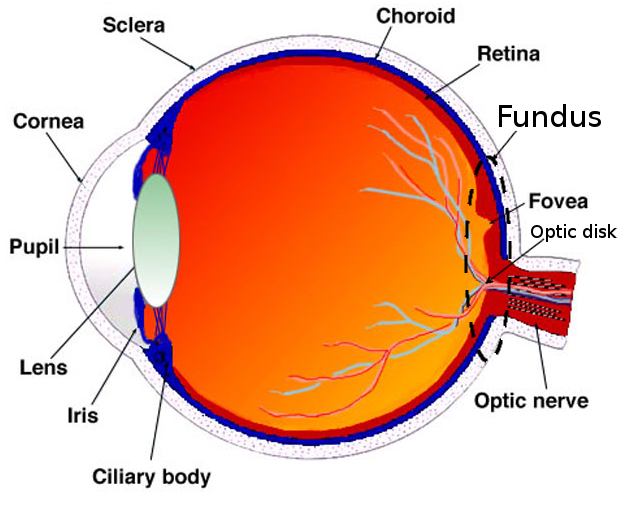
\includegraphics[width=0.45\textwidth]{cross_section_eye}}
    \subfloat[]{
    \label{fig:healthyeyefundus}
    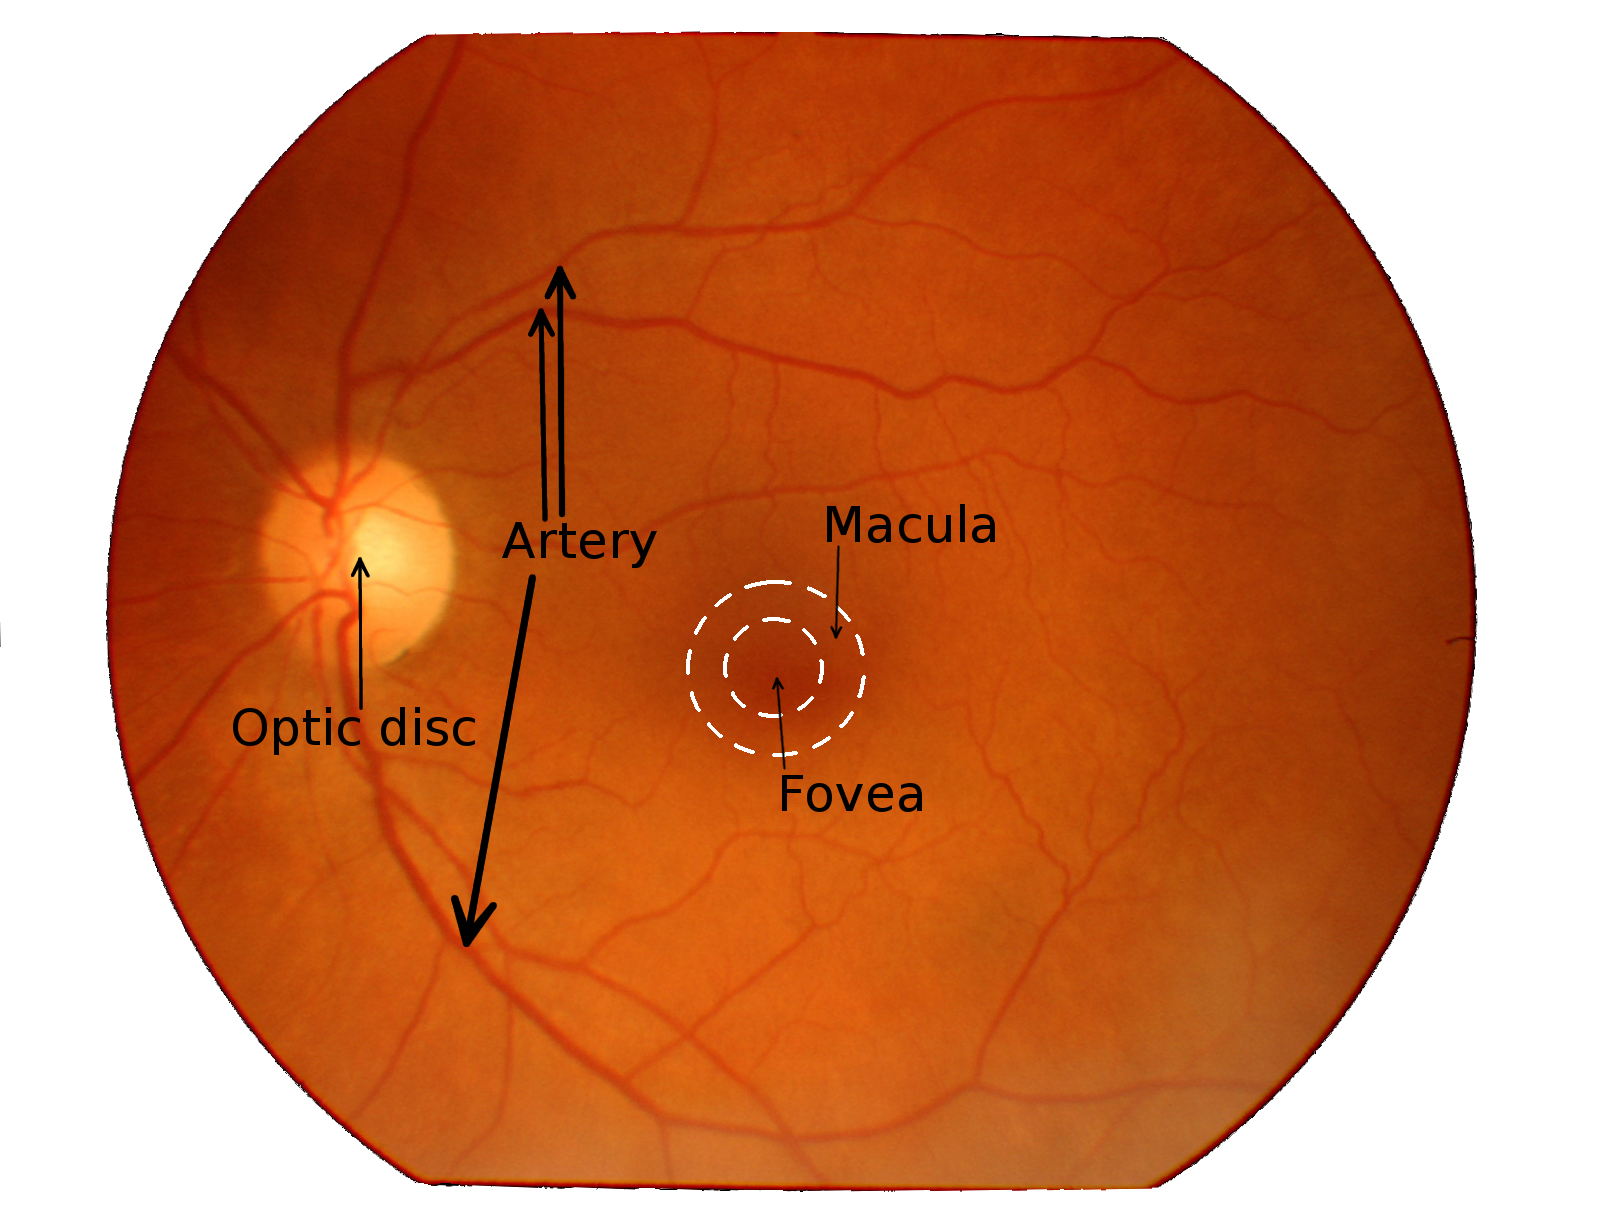
\includegraphics[width=0.45\textwidth]{healthyeyefundus}}
     
  \caption[moving]{Structure of the human eye:
  \subref{fig:cross_section_eye} cross section of the eye (modified from~\cite{Kolb}),
  \subref{fig:healthyeyefundus} structure of the fundus.
  
  
  \label{fig:eyestructure}}
}\end{figure}



\subsection{Optic disc detection}
\label{subsec:opticdisc}
Optic disc is very similar to exudates in terms of color and intensity, so detection
and masking of the optic disk is an important preprocessing step in exudate detection.
There are papers dedicated to the localisation of the optic disk~\cite{Sekhar:2008},
and it is also covered in papers concerning the detection of other parts of the eye
fundus, such as exudates~\cite{Walter:2002}.

The method used in this thesis is based on the brightness of the optic disk, and the vertical blood vessels inside it.
The horizontal image gradient is calculated using Sobel operator\cite{Perra:2005}, the result is shown in 
Figure~\ref{fig:opticdisk_gradient}. The image is then divided into slightly overlapping square 
areas with a side of 140 pixels. The area
with the highest sum of gradients is considered as region of interest, i.e. to hold the optic disk.
This is because the dark blood vessels inside the bright optic disk result in a strong horizontal
gradient. Images with a ``camera glare``, i.e. a high intensity strip in the corner of the eye fundus
are problematic, as that area also has a high horizontal gradient. An example region of interest is shown in Figure~\ref{fig:opticdisk_ROI}.

Inside the area of highest sum of horizontal gradients, the pixel with the highest intensity is considered
to be inside the optic disk. This pixel is then used as the center of a circle that will mask out the optic disk.
The final masking result is shown in Figure~\ref{fig:opticdisk_masked}.

\begin{figure}[ht]
\centering
{
  \subfloat[]{
     \label{fig:opticdisk_gradient}
     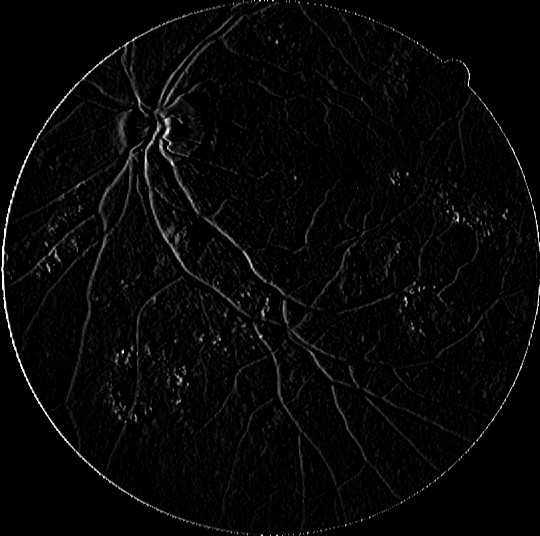
\includegraphics[width=0.45\textwidth]{OP_gradient}}
  \subfloat[]{
     \label{fig:opticdisk_ROI}
     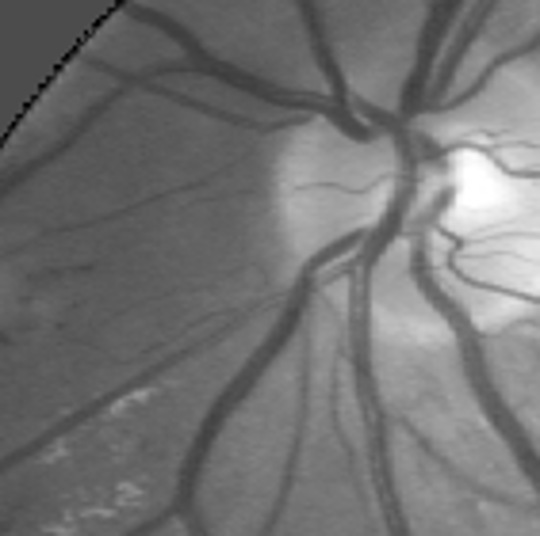
\includegraphics[width=0.45\textwidth]{OP_ROI}}
     
     
  \subfloat[]{
     \label{fig:opticdisk_masked}
     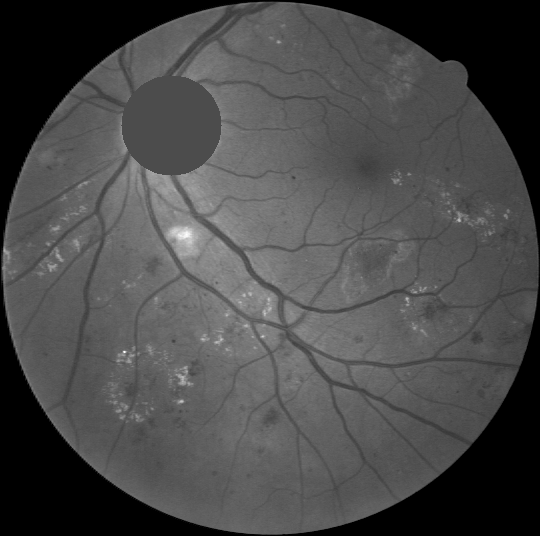
\includegraphics[width=0.45\textwidth]{OP_masked}}

  \caption[moving]{Locating and masking the optic disk:
  \subref{fig:opticdisk_gradient} horizontal gradient,
  \subref{fig:opticdisk_ROI} region of interest,
  \subref{fig:opticdisk_masked} optic disk masked out.}
  \label{fig:opticdisk}
}\end{figure}


\subsection{Blood vessel detection}
\label{subsec:vesselmask}

The issue of blood vessel detection in fundus images has been a popular topic of research~\cite{Zana:1999,Staal:2004,Niemeijer:2004}.

In the context of this thesis, however, the purpose of blood vessel detection is to create a mask, and to use that mask to remove false
positives from exudate segmentation results. For example, edge detection techniques often highlight the
borders of vessels as well as exudates. For this purpose, accurate vessel detection itself is not important and
including other dark areas of the image is even beneficial.

The mask is formed by first using contrast-limited adaptive histogram equalization\linebreak(CLAHE)~\cite{Reza:2004} to enhance
contrast in the green channel of the image, the result for this is shown in Figure~\ref{fig:vesselmask_adaptive}. This
contrast enhanced image is then thresholded with Otsu's method~\cite{Otsu:1975}, which separates the image into foreground
and background by minimizing the intra-class variance. This results in all the vessels and other darker areas classified as background,
and all brighter areas classified as foreground. This is shown in Figure~\ref{fig:vesselmask_threshold}.
To create a binary mask of the darker areas, we use the complement of this thresholded image. The final version of the
mask is shown in Figure~\ref{fig:vesselmask_complement}.

This method is inadequate for blood vessel detection as it also includes other darker areas of the image, 
such as the fovea. As a mask, however, it clearly reduces the amount of false positives in exudate segmentation results.
It also does not remove true positives, as only the darker areas of the image are included in the mask.

\begin{figure}[ht]
\centering
{
  \subfloat[]{
     \label{fig:vesselmask_adaptive}
     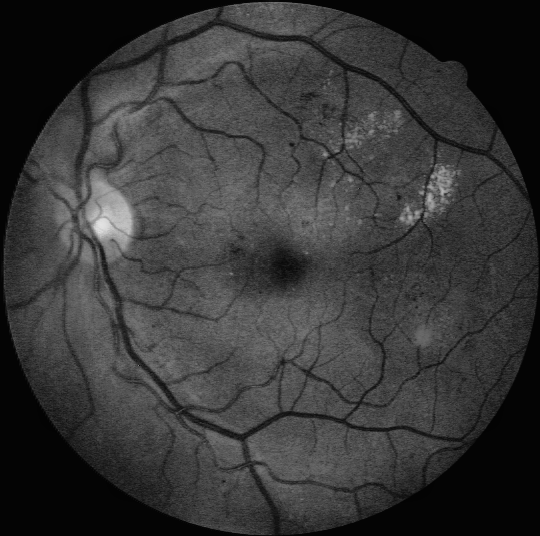
\includegraphics[width=0.45\textwidth]{vesselmask_adaptive}}
  \subfloat[]{
     \label{fig:vesselmask_threshold}
     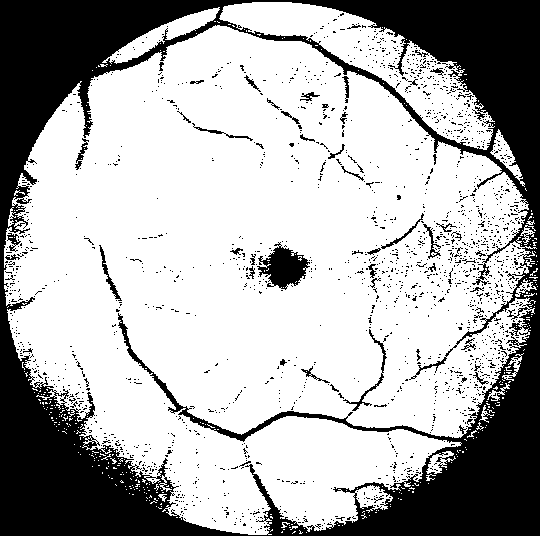
\includegraphics[width=0.45\textwidth]{vesselmask_threshold}}
     
     
  \subfloat[]{
     \label{fig:vesselmask_complement}
     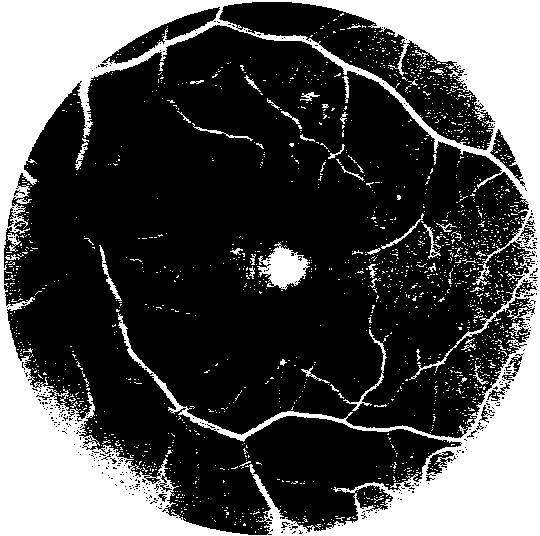
\includegraphics[width=0.45\textwidth]{vesselmask_complement}}

  \caption[moving]{Creating the blood vessel mask:
  \subref{fig:vesselmask_adaptive} CLAHE,
  \subref{fig:vesselmask_threshold} thresholding using Otsu's method,
  \subref{fig:vesselmask_complement} the final mask, complement of thresholded image.}
  \label{fig:vesselmask}
}\end{figure}

\subsection{Color transform}
\label{subsec:colortransform}
The human eye is capable of correcting the effect of varying light sources (illuminants) while perceiving color~\cite{Foster:2011}.
In contrast, an image of an object taken under different light sources is perceived differently in terms of color by a computer.
This promotes the normalization of color features in image sets where there's high variation in color properties. In this thesis,
the use of color normalization is motivated by the variation of the color of the pigment epithelium layer in the eye fundus.

The illumination and general color properties of the eye fundus images vary quite heavily.
To be able to effectively use color features in teaching a classifier, the variance between images needs to be minimized.
This is achieved by estimating the illuminant by applying the gray-world assumption~\cite{Buchsbaum:1980}:
\textit{the average reflectance in a scene under a neutral light source is achromatic.} While this does not hold true in the case of eye fundus
images, the application had positive results in terms of color feature normalization as seen in Figure~\ref{fig:colortransform}. Normalization was 
done by multiplying each channel with a coefficient defined as $ K_r = I_{avg} / r_{avg}$, where $I_{avg}$ is the mean
of all RGB-values in the image, and $r_{avg}$ is the mean of the specific channel.

\begin{figure}[ht]
\centering
{
  \subfloat[]{
     \label{fig:original_010}
     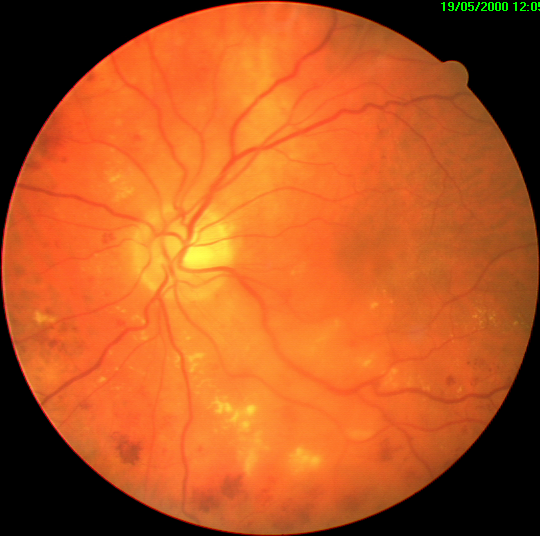
\includegraphics[width=0.45\textwidth]{original_010}}     
  \subfloat[]{
     \label{fig:color_010}
     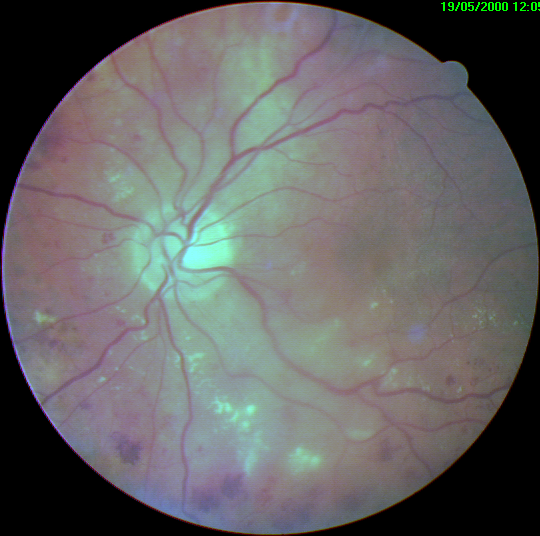
\includegraphics[width=0.45\textwidth]{color_010}}
     
  \subfloat[]{
     \label{fig:original_011}
     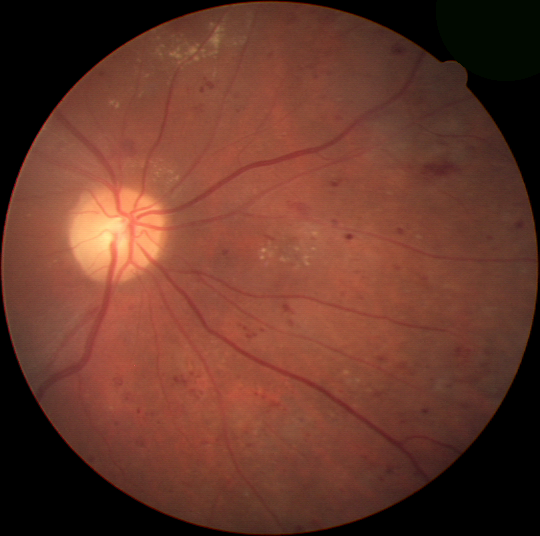
\includegraphics[width=0.45\textwidth]{original_011}}     
  \subfloat[]{
     \label{fig:color_011}
     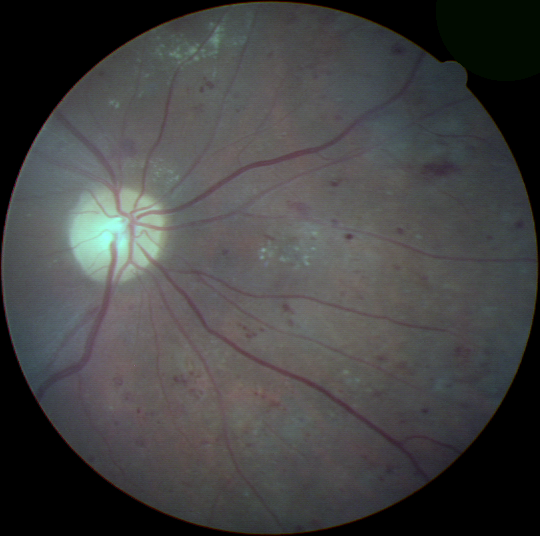
\includegraphics[width=0.45\textwidth]{color_011}}

  \caption[moving]{Color space transform: Original images on the left, adjusted images on the right.}  
  \label{fig:colortransform}
}\end{figure}


\subsection{Unsupervised image segmentation methods}
\label{subsec:unsupervised}
% An unsupervised method doesn't hold any information of the features it seeks, nor does it have any ''expectations'' of the image.
% It perform the same operations on each image with the object of clustering the data into meaningful sets.
% 
% Most edge detection methods are unsupervised algorithms. Edge is defined as a sharp change in image and color intensity, 
% and the purpose of an edge detection algorithm is to emphasize and detect those sharp changes in an image. In an eye fundus image,
% this would include the exudates, but also the borders of the blood vessels and optic disc. As such, edge detection isn't
% sufficient for exudate detection since these unwanted regions need to be subtracted from the initial result. During this study,
% this is accomplished with the mask acquired in Section~\ref{subsec:vesselmask}.

\subsubsection{Kirsch operator}

Edge detection operators that only detect gradients in specified directions are called compass operators.
Kirsch operator applies a compass operator in eight directions by rotating a mask in 45$^{\circ}$ shifts.~\cite{Jain:1989}
It is defined as:

\[
K_1 = \begin{bmatrix}
  5 & 5 & 5 \\
 -3 & 0 &-3 \\
 -3 &-3 &-3 
\end{bmatrix}, 
K_2 = \begin{bmatrix}
  5 & 5 &-3 \\
  5 & 0 &-3 \\
 -3 &-3 &-3 
\end{bmatrix} 
, ..., K_8 = \begin{bmatrix}
 -3 & 5 & 5 \\
 -3 & 0 & 5 \\
 -3 &-3 &-3 
\end{bmatrix}.

\]      
\vspace{-20mm}

\subsubsection{Morphological operations}

Mathematical morphology operations use a structuring element to perform an operation on an input image.
Most morphology operations are based the two basic morphological operations, dilation and erosion.
Top-hat transform is an operation that highlights bright areas in an image, where as bottom-hat
(also known as black top-hat) operation highlights the dim areas of an image.~\cite{Bai:2012}
These transforms are defined as follows:
%\vspace{-2mm}
\begin{equation}\label{eq:tophat}
\begin{split}
TopHat(f,B) = f - (f \circ B)
\end{split}
\end{equation}
\vspace{-25mm}

\begin{equation}\label{eq:bottomhat}
\begin{split}
BottomHat(f,B) = (f \bullet B) - f
\end{split}
\end{equation}
\vspace{-5mm}


where $f$ is the input image, $B$ is the structuring element, $\circ$ denotes the opening operation and $\bullet$
denotes the closing operation. Opening and closing are standard operations based on dilation and erosion, and they are defined in~\cite{Bai:2012}.

The exudate detection method proposed in~\cite{Eadgahi:2012} was also implemented, except for the optic disc detection, for which 
the method described in Section~\ref{subsec:opticdisc} was used. The method is designed to use the top-hat operation to highlight the exudates, 
and the bottom-hat operation to highlight and ultimately remove dim areas, e.g. vessels from the results. The method is defined as follows:

%\vspace{-12mm}
\begin{equation}\label{eq:mehdi}
\begin{split}
F(f) = TopHat(f) - BottomHat(f)
\end{split}
\end{equation}
%\vspace{-10mm}

where $Tophat(f)$ and $BottomHat(f)$ denote Equations \ref{eq:tophat} and \ref{eq:bottomhat}, respectively.
Unlike in~\cite{Eadgahi:2012}, thresholding is applied after these operations to enable evaluation by creating a binary representation
of the results.

\subsection{Supervised methods}
\label{subsec:supervised}
% Before a supervised method (or its classifier) can be used in classification, it needs to be trained. A specific training set
% of labeled images is used to teach the classifier. The method then extracts features from the training images, and generally forms a model
% for each used label. For example, to describe a fruit you might use its color and shape. You ''teach'' the method what each
% fruit looks like by labeling a set of training images. The classifier learns which features describe each label. Yellow and round equals orange,
% yellow and long equals banana, green and round equals apple. After training, the classifier can be used to classify new images.

Color, edge and texture features were used to teach the classifiers of the supervised methods.
Color was extracted from the image as pixel-specific RGB-values. Edge was represented with the differential of the
maximum and minimum value in a 3-by-3 neighborhood (implemented with \textit{rangefilt}-function in MATLAB ~\cite{rangefilt}).
Location-invariant local binary patterns (LBP)~\cite{Ojala:2000} were used for texture.

\subsubsection{Na�ve Bayes}

Na�ve Bayes is a probabilistic classifier that gets its name from the assumption that all features are independent from each other. Each feature
contributes to the classification regardless of the absence or presence of other features. As the name also implies, the Na�ve Bayes classifier
uses the Bayesian theorem as the basis of classification.~\cite{Murphy:2006}

The Na�ve Bayes classifier calculates the posterior probability for the sample to belong in each of the possible classes based on its features, and then
classifies the sample to the class with the highest posterior probability. The classes are modeled with a single probability density function, and in the case of
binary pixel classification, the classes are foreground and background. In this thesis, exudates represent the foreground and the rest 
is considered the background. The posterior probability is calculated with the Bayesian theorem as follows:

\begin{equation}\label{eq:naivebayes}
\begin{split}
p(C_1) = \frac{P(C_1)p(\overline{x}|C_1)}{P(C_1)p(\overline{x}|C_1) + P(C_2)p(\overline{x}|C_2)}
\end{split}
\end{equation}

where $ p(C_1) $ is the posterior probability and $ P(C_1) $ is the prior probability for the sample to belong in class one, and $ p(\overline{x}|C_1) $
denotes the conditional probability of the feature vector having the values of the sample pixel, if it were of class one.


\subsubsection{Gaussian Mixture Models}

A Gaussian mixture model (GMM) is a single probability density function (pdf) that describes a weighted sum of multiple Gaussian pdfs~\cite{Reynolds:2009}.
When using a GMM to model image classes (more specifically, class-conditional pdfs), parameters of the underlying Gaussian pdfs are estimated by fitting the
model to training data. After the formation of the model, it is possible to use Bayesian classification to classify pixels to the given classes.

Application, parameter estimation and performance of a classifier using GMMs and\linebreak Bayesian classification is discussed in~\cite{paalanen2006feature}.
GMMBayes Toolbox~\cite{Paalanen:2004} is a MATLAB implementation of these methods. For parameter estimation, Expectation Maximization (EM), Figuero-Jain (FJ)
and greedy EM algorithms are implemented in the toolbox and described in both~\cite{paalanen2006feature} and~\cite{Paalanen:2004}. The main difference between
these algorithms is that EM requires a fixed amount of Gaussian components, while FJ estimates the amount (maximum amount is fixed in the implementation).
In this thesis, only FJ is used.

\subsection{Evaluation metrics}
\label{subsec:evaluation}

In evaluation, correctly classified samples can be split into true positives and true negatives. Errors are then similarly split
into false positives and false negatives. In this thesis, true positives are findings correctly classified as exudates 
in the segmentation results, and true negatives are consequently findings correctly classified as the background. False
negatives are classified as background in the results, but are actually positive (classified as exudate) in the ground truth, and
false positives are classified as positive in the results, when they are in fact background~\cite{Fawcett:2006}. These terms are illustrated with
an error matrix shown in Table ~\ref{tab:truepositive}.

\begin{table}[hpt]
\begin{center}
\caption{General error matrix\label{tab:truepositive}}

\begin{tabular}{cc|c|c|c|c|l}
\cline{3-4}
& & \multicolumn{2}{ c| }{Ground truth} \\ \cline{3-4}
& & Positive & Negative  \\ \cline{1-4}
\multicolumn{1}{ |c| }{\multirow{}{}{Tests} } &
\multicolumn{1}{ |c| }{Positive} & True Positive (TP)& False Positive (FP) \\ \cline{2-4}
\multicolumn{1}{ |c  }{}  &
\multicolumn{1}{ |c| }{Negative} & False Negative (FN)& True Negative (TN) \\ \cline{1-4}

\end{tabular}
\end{center}
\end{table}


% Sensitivity represents the amount of samples correctly classified as positive. and specificity in turn represents
% the amount correctly classified as negative. Both have values ranging from 0 to 1, where 1 represents the best possible
% result.
Sensitivity represents the proportion of samples correctly classified as positive. Its values range from 0 to 1, where 1
means all foreground samples were correctly classified. Specificity in turn represents the proportion of background pixels
correctly described as negative. Its values also range from 0 to 1, where 1 means all the background pixels were correctly classified. ~\cite{Fawcett:2006}
They are defined as:

% \vspace{-1mm}
\begin{equation}\label{eq:sensitivity}
\text{Sensitivity} = \frac{TP}{TP+FN}
\end{equation}
\vspace{-2mm}
\begin{equation} \label{eq:specificity}
\text{Specificity} = \frac{TN}{TN+FP}
\end{equation}

The Dice coefficient~\cite{Dice:1945}, Jaccard index and F-score all measure set agreement, representing the success of segmentation with a single number.
All of these coefficients can have values from the range [0,1], where 0 indicates no similarities, and 1 indicates perfect agreement. The coefficients
are defined as follows:
\begin{equation}\label{eq:dice}
\begin{split}
\text{Dice} = \frac{2|A\cap B|}{|A| + |B|}
\end{split}
\end{equation}
%\vspace{-2mm}
\begin{equation}\label{eq:jaccard}
\begin{split}
\text{Jaccard} = \frac{|A\cap B|}{|A\cup B|}
\end{split}
\end{equation}
%\vspace{-2mm}
\begin{equation}\label{eq:fscore}
\begin{split}
\text{F-score} = \frac{2PR}{P + R}
\end{split}
\end{equation}

where A is the segmented set, and B is the ground truth, P stands for precision and R stands for recall (sensitivity).

\section{EXPERIMENTS AND RESULTS}
\label{sec:experiments}

\subsection{The ground truth}
\label{subsec:groundtruth}
To enable the comparison of results and sensitivity analysis,
more inaccurate ground truths were made by hand, using the Bristol ground truth as a basis. Instead of the original color images, markings for the inaccurate ground truth were
made on the black-and-white images of the Bristol ground truth. This was to ensure every exudate present in the Bristol ground truth was to be
also present in the inaccurate ground truth. Markings were done by grouping clusters of exudates together, and marking single exudates more loosely.
This is illustrated in Figure~\ref{fig:groundtruth}.

To create a basis for more comprehensive testing, different stages of inaccurate ground truths were created by dilating the accurate
ground truth. Three different stages were created; one, three and five iterations of dilation by a disk-shaped structuring element, with a radius of 1 pixel.
The dilation was restricted to stay inside the inaccurate ground truth.

The accuracy of the ground truth has a direct impact on training and performance of supervised methods. In general, the inaccurate ground truth 
will mean a significant amount of background samples close to exudates will be categorized as positive. This will result in higher 
variation of feature distributions and an increase of false positives.

\begin{figure}[ht]
\centering
{
  \subfloat[]{
     \label{fig:bristol_gt}
     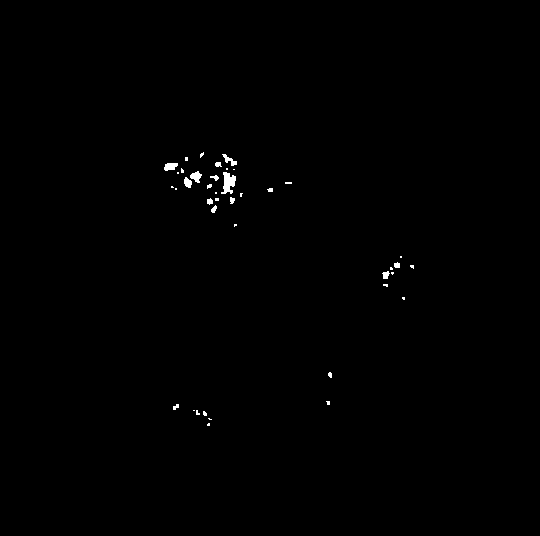
\includegraphics[width=0.45\textwidth]{bristol_groundtruth}}
  \subfloat[]{
     \label{fig:inaccurate_gt}
     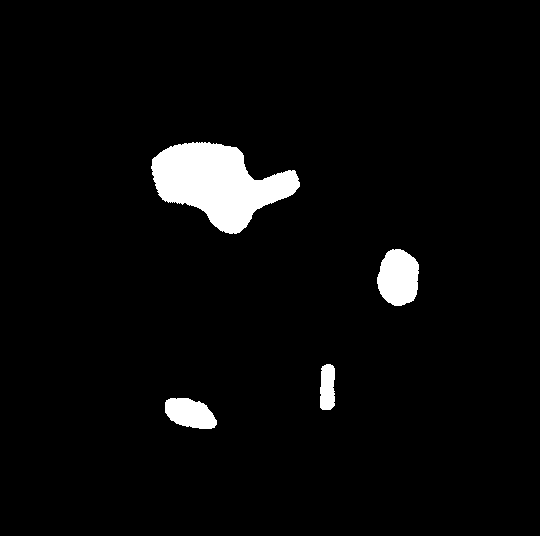
\includegraphics[width=0.45\textwidth]{inaccurate_groundtruth}}
     
  \caption[moving]{Ground truths:
  \subref{fig:bristol_gt} Original accurate ground truth
  \subref{fig:inaccurate_gt} The most inaccurate ground truth }
  \label{fig:groundtruth}

}\end{figure}

\subsection{Supervised image segmentation methods}

\subsubsection{Test settings}
\label{subsubsec:settings}
Preprocessing was kept to a minimum as only the timestamp was removed from the eye fundus images.
As the optic disk's color is very close to the exudates, a mask was generated with the method described in
Sec.~\ref{subsec:opticdisc}. The eye outline was also included in the mask, as it was included in the results
by edge detection methods. Vessels were not included in the mask.

The amount of background pixels in the images is considerably higher than the amount of exudate pixels.
This was balanced by applying sampling to the training data, using equal amounts of background and exudate pixels.
All exudate pixels were used, and background pixels were selected randomly.

Classifiers were trained with color, edge and texture features, and with the combination of the three. The feature extraction
methods are described in Sec.~\ref{subsec:supervised}. No contrast enhancement was used, so raw color information
from the image was used as the color feature.

The Bristol image set was divided into two parts, using one half for training and the other half for evaluation,
and then vice versa. This was done to study the effect the selection of training data has on the results.
Classifiers were trained with each level of inaccurate ground truth described in Sec.~\ref{subsec:groundtruth}.
Two different image sets were used; the original Bristol images, and the color-normalized images. The colors were adjusted
with the method described in Sec.~\ref{subsec:colortransform}, with the objective of reducing the color variation in the images.
With this setup, each calculation used a specific ground truth accuracy, image set, and teaching set.

\subsubsection{Results and discussion}

Using inaccurate ground truth was expected to result in more false positives in image segmentation results.
This can be seen in the results as an increase in sensitivity and a decrease in specificity with all features and classifiers 
when the level of inaccuracy in the ground truth increases. This is also visible in the image-specific results shown in Appendices~\ref{app:bayes} and~\ref{app:gmmbayes}.
All image segmentation methods and classifiers behave similarly in this regard, having gradually more and more false positives in their segmentation results
as the ground truth is made more inaccurate.

Comparing the sensitivity and specificity of Na�ve-Bayes and GMM-Bayes classifiers shown in Figures~\ref{fig:bayes} and~\ref{fig:gmmbayes},
a slighty higher performance of color feature GMM-Bayes classifier can be seen. The Na�ve-Bayes edge-classifier on the other hand,
is outperforming other single-feature trained classifier and even the classifier with all the features included. It is worth noting that the 
linear progression of Na�ve-Bayes' sensitivity and specificity as the ground truth becomes more inaccurate.
Based on the specificity of the texture-based classifiers, their performance was below the others. The image-specific results
explain this, as the texture-based classifier behave similarly to a random classifier. This could be because of the feature's
variation in the training set, but this was not confirmed. It is worth noting that images without exudates are excluded from these results,
as they have no other effect than decreasing the average performance. It is worth noting that it is necessary to also include the exudate-free 
images when developing a practical application.

Color normalization's impact on the results was negligible. It was expected to improve the performance of a classifier using the color feature by 
reducing the color variance of the exudates and background. However, results with Na�ve-Bayes are almost identical between the image sets,
and no clear improvement can be seen from the results of GMM-Bayes.

In the Figures~\ref{fig:bayes} and~\ref{fig:gmmbayes}, selection of training data is represented via the dotted or filled line.
Generally, the selection of training data had a minor impact on the results. Performance of both methods' classifiers using edge feature, however,
changed drastically when using the most inaccurate ground truth. This can be seen as a drop in specificity. Selection of training data also had a
noticeable effect on the performance of GMM-Bayes classifier using all features. For others, the selection of training data did not appear to have a
meaningful effect.

\begin{figure}[ht]
{
  \subfloat[]{
     \label{fig:bayes_sens}
     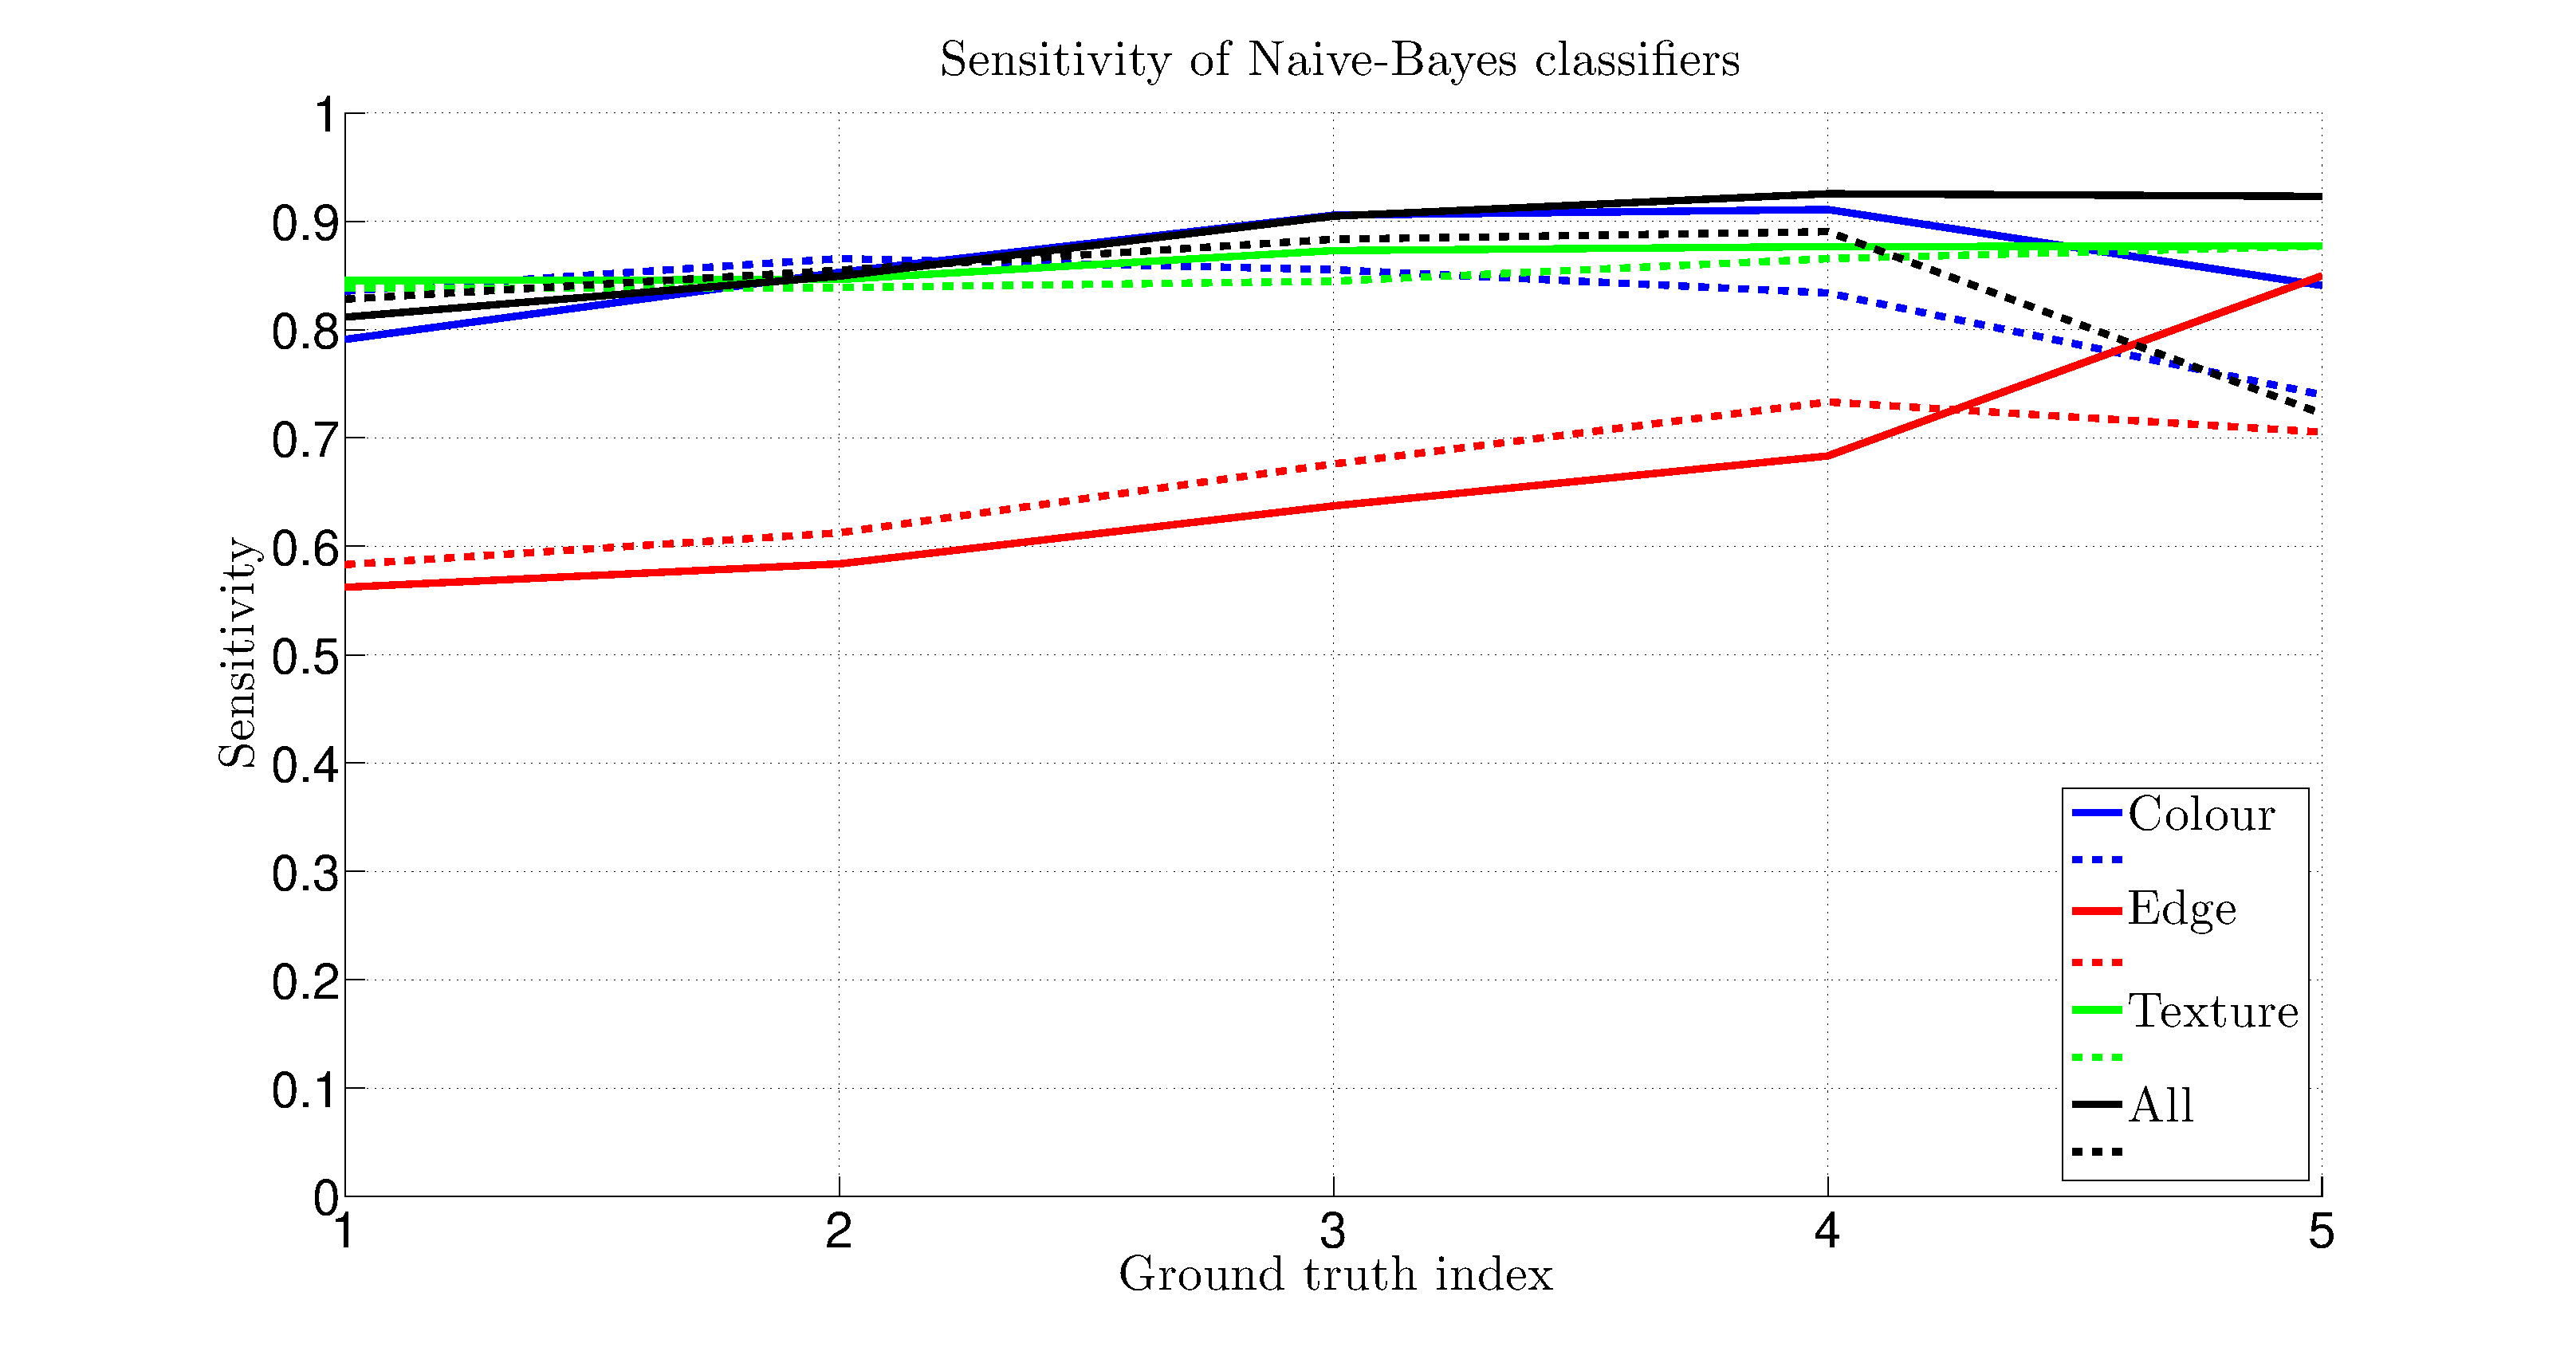
\includegraphics[width=0.95\textwidth]{hist_bayes_sens_imgset1}}
  
  \subfloat[]{
     \label{fig:bayes_spec}
     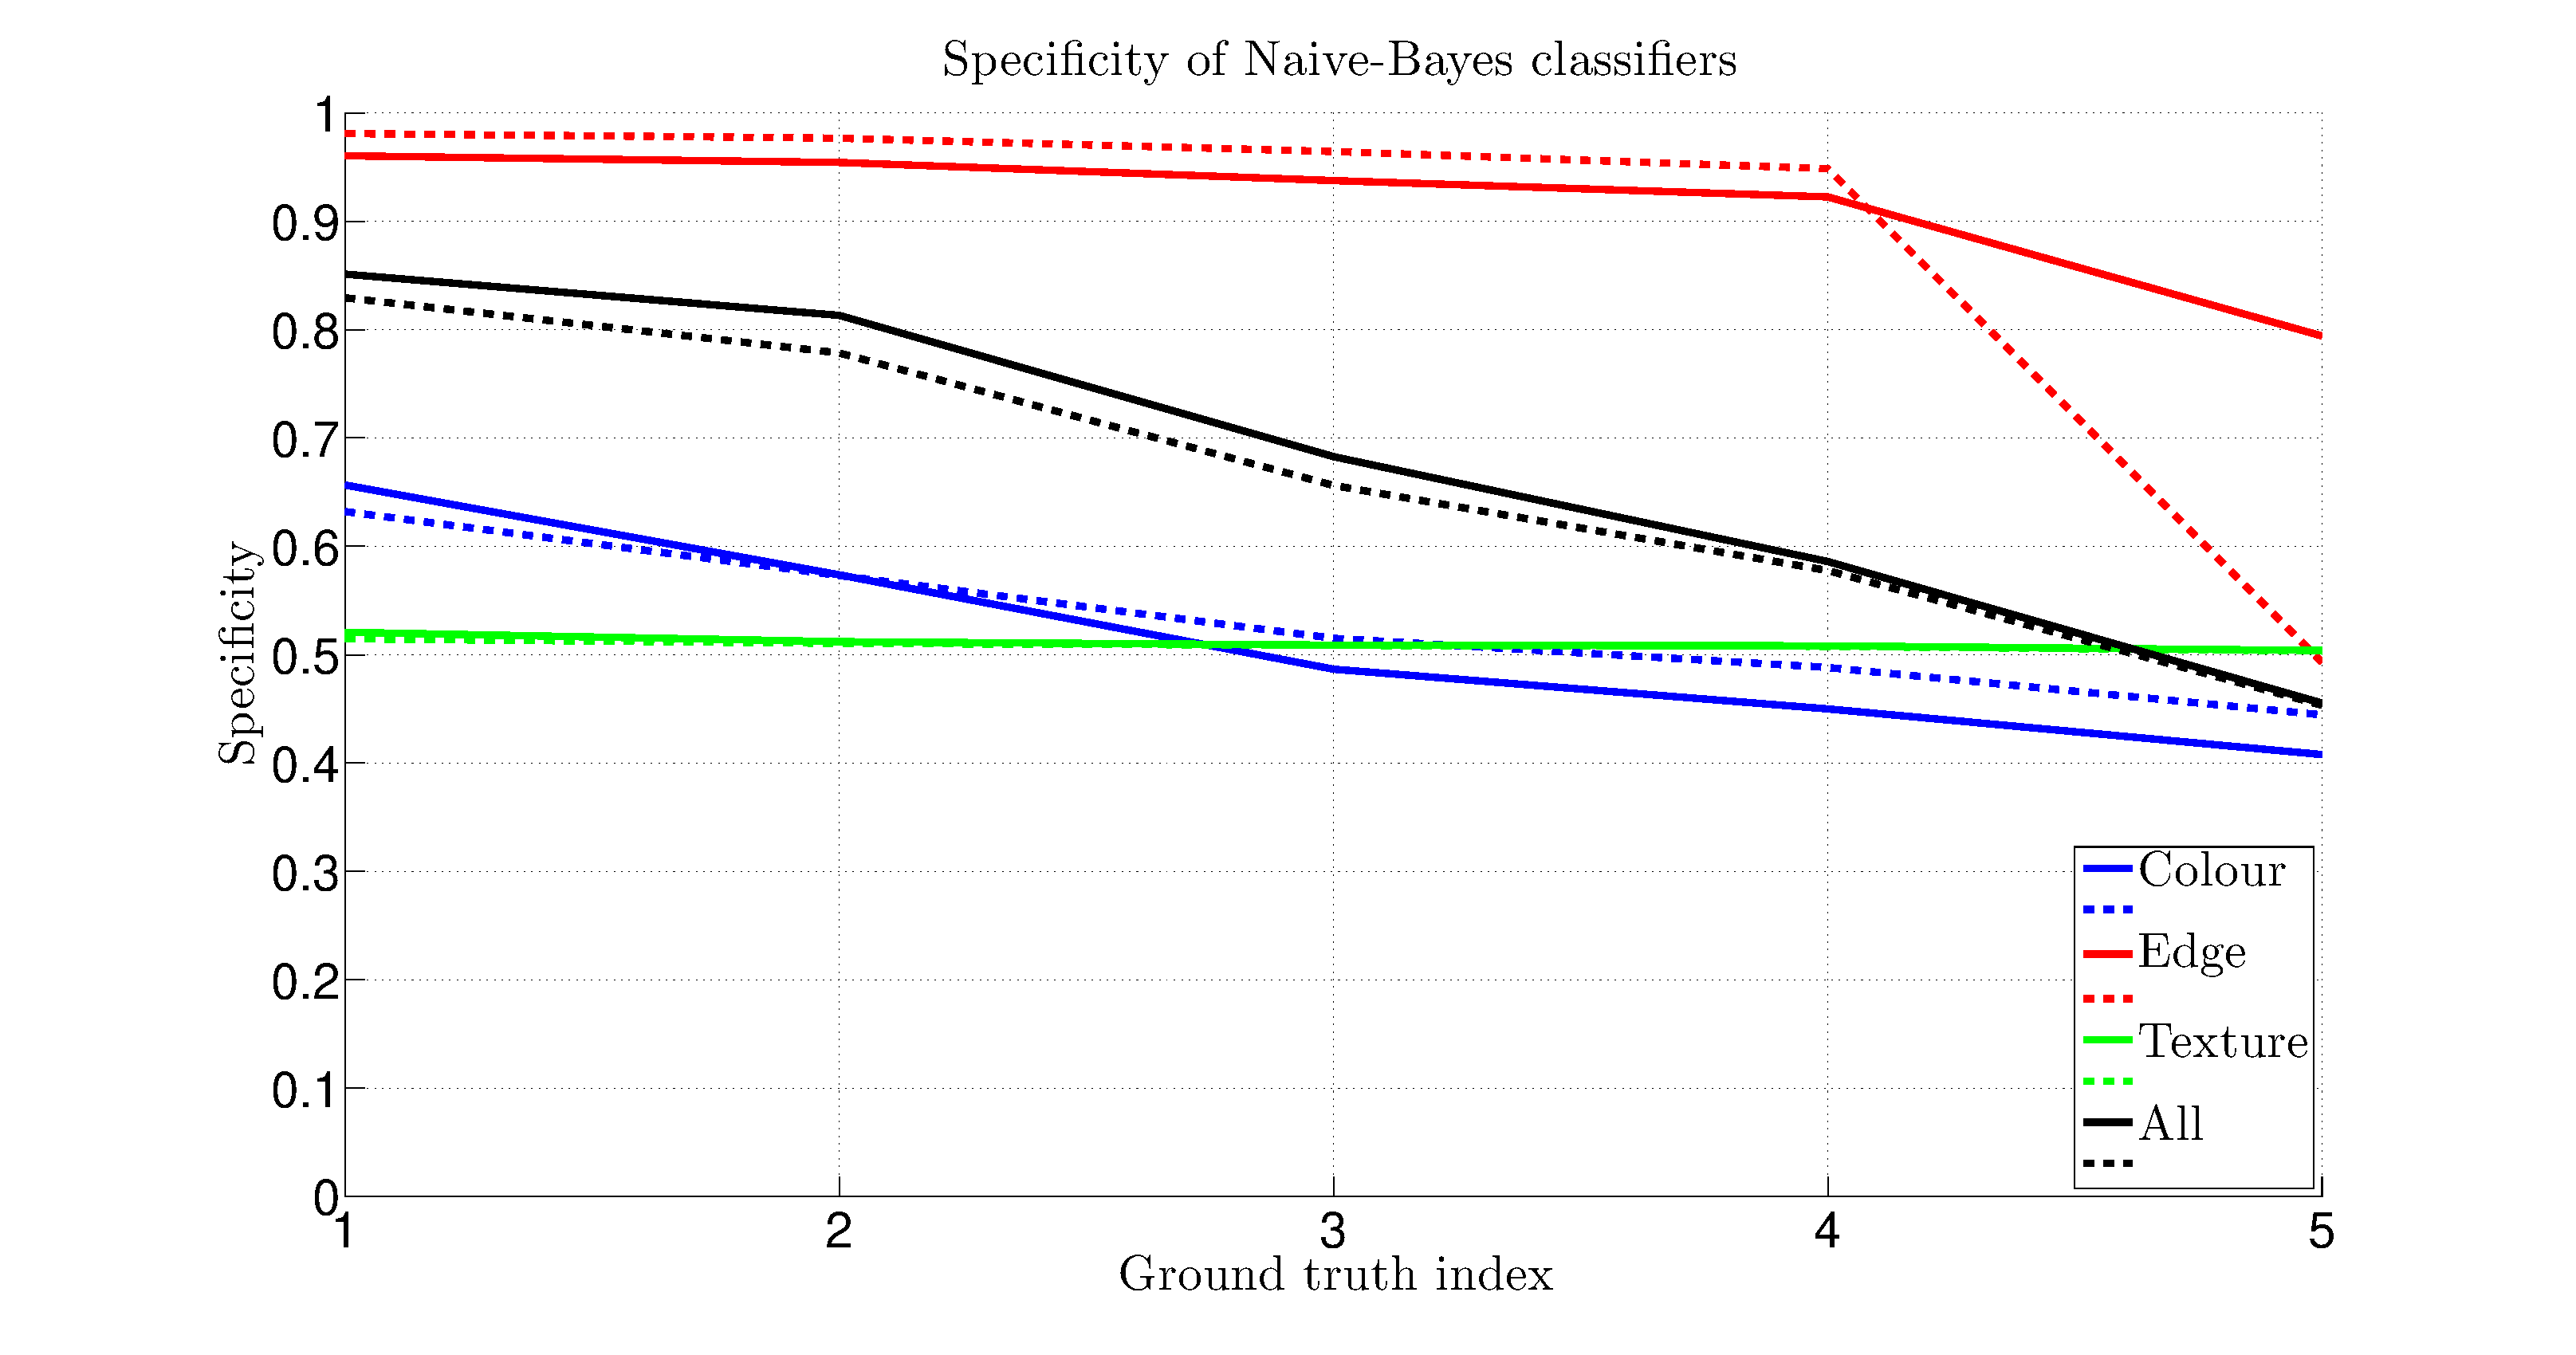
\includegraphics[width=0.95\textwidth]{hist_bayes_spec_imgset1}}
     
  \caption[moving]{Performance of Na�ve-Bayes classifiers:
  \subref{fig:bayes_sens} Sensitivity
  \subref{fig:bayes_spec} Specificity. Note that these graphs represent
  the methods' performance over images that have exudates present. The original
  Bristol ground truth is on the left on the x-axis, and the most inaccurate
  ground truth is on the right. Solid and dotted lines represent the use of different
  training/testing sets, as described in Section~\ref{subsubsec:settings}. }
  \label{fig:bayes}

}\end{figure}

\begin{figure}[ht]
{
  \subfloat[]{
     \label{fig:gmmbayes_sens}
     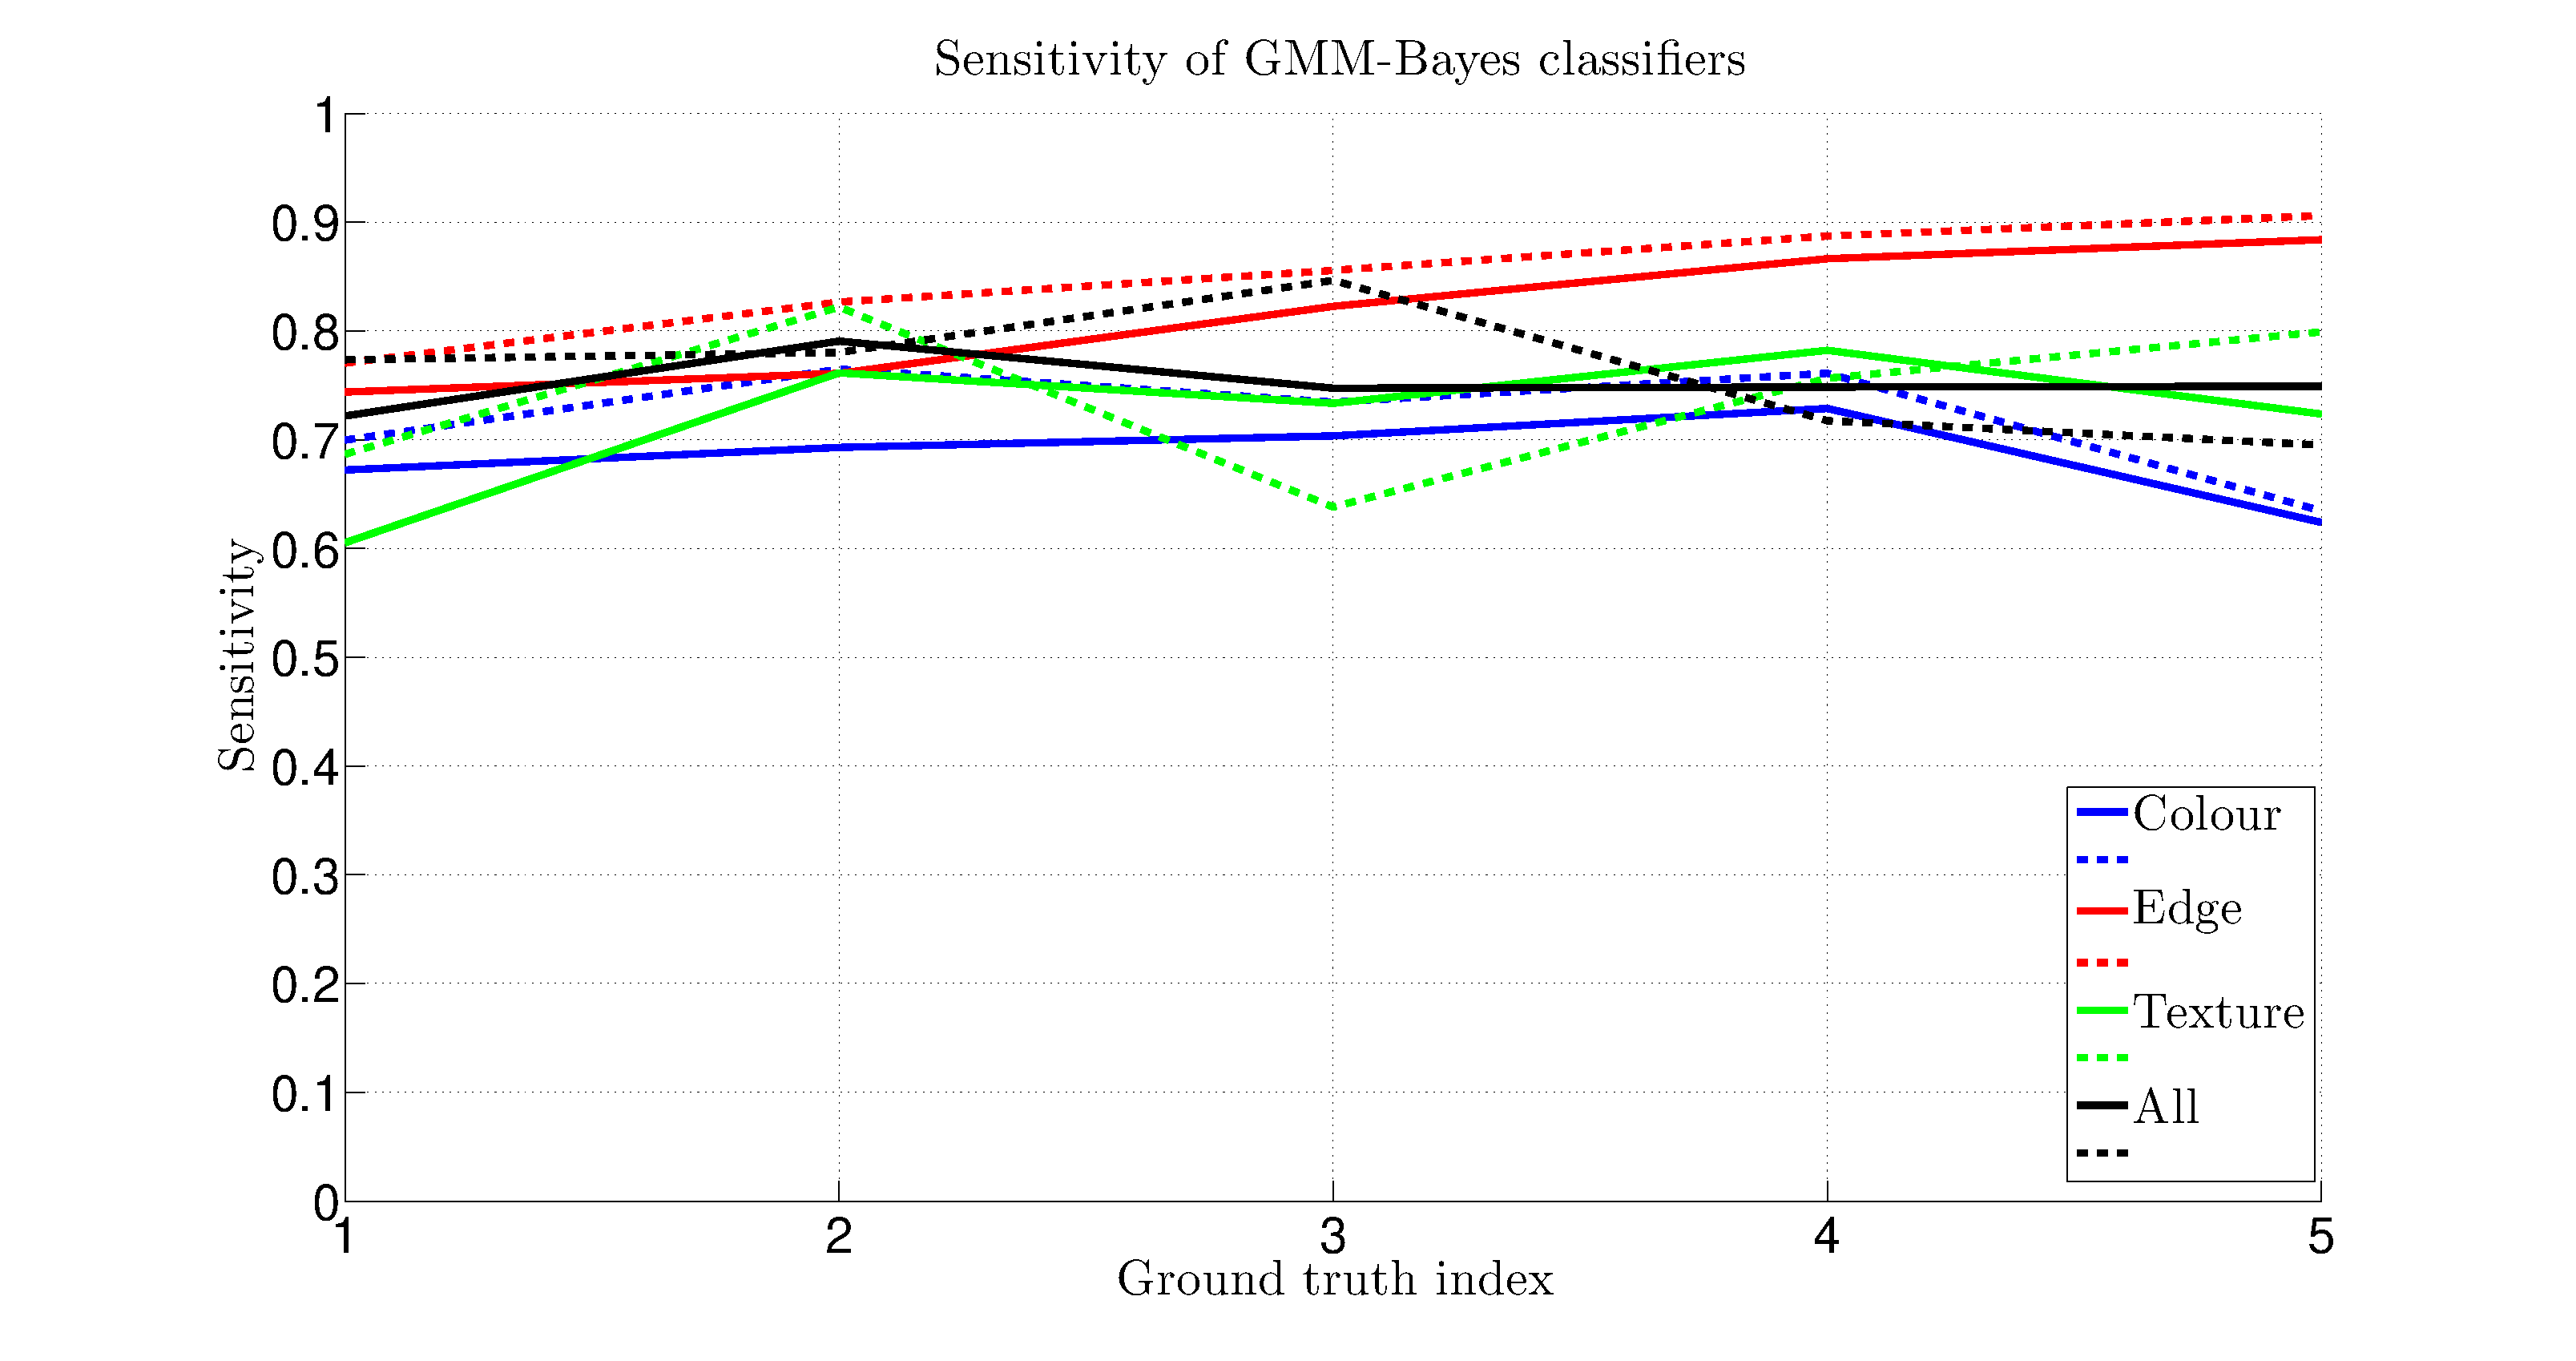
\includegraphics[width=0.95\textwidth]{hist_gmmbayes_sens_imgset1}}
  
  \subfloat[]{
     \label{fig:gmmbayes_spec}
     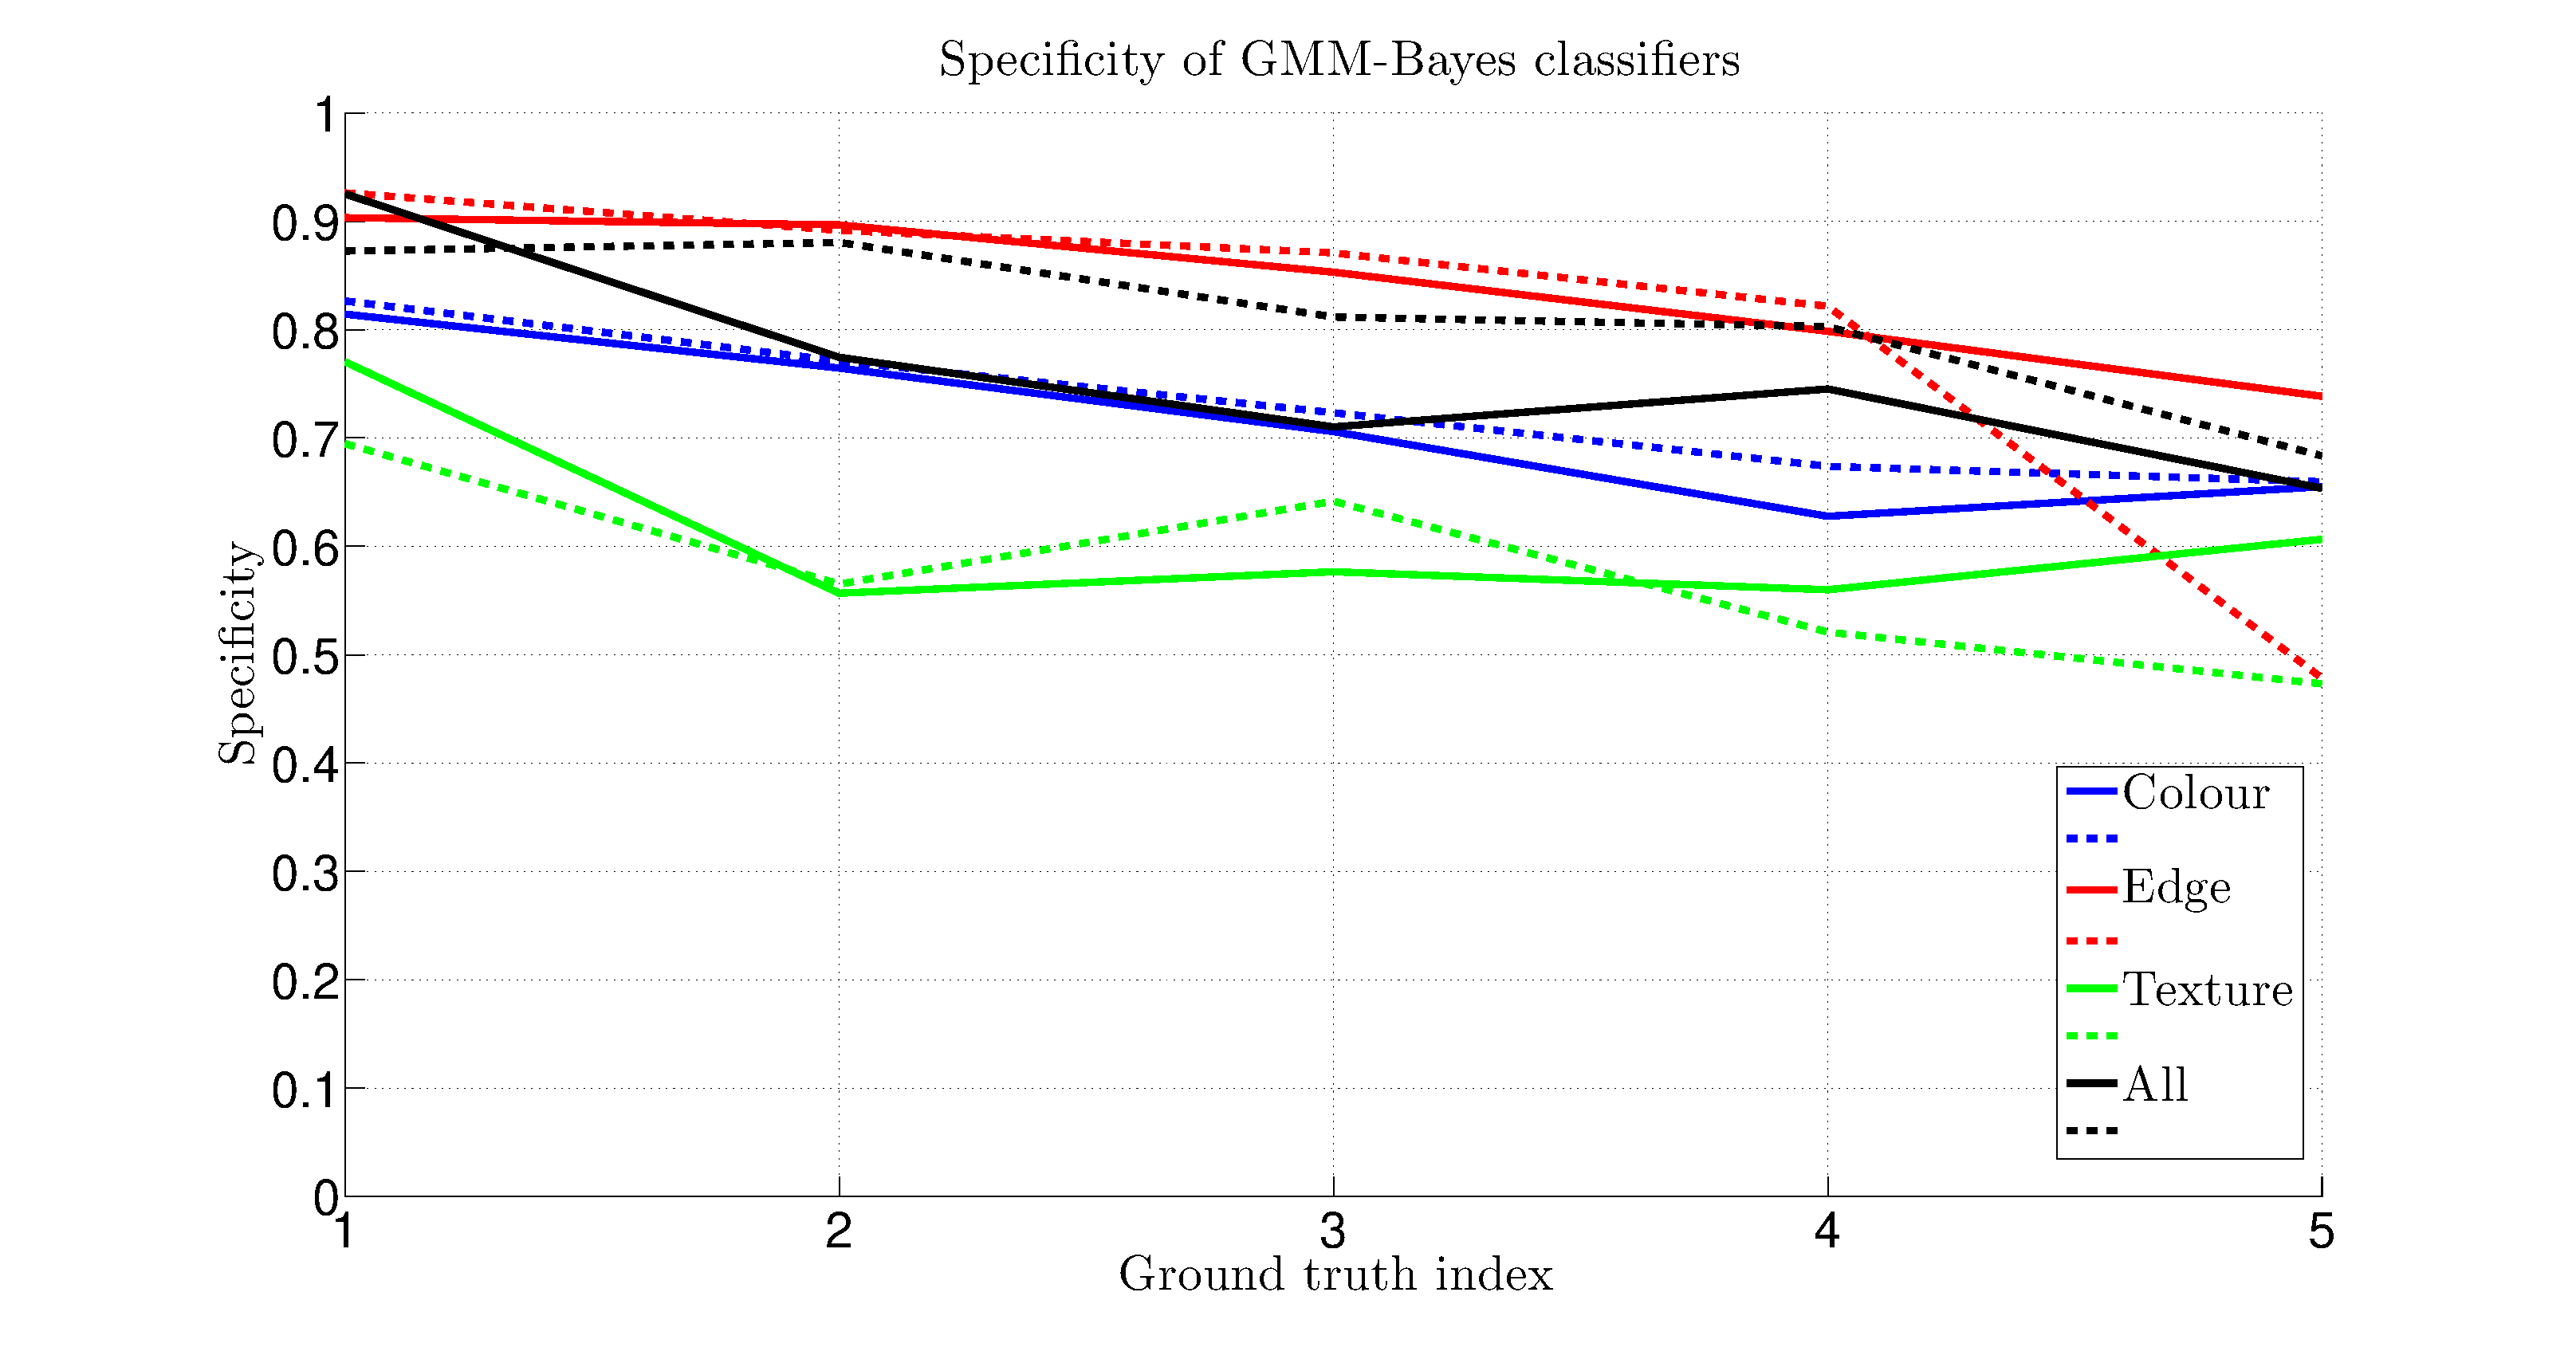
\includegraphics[width=0.95\textwidth]{hist_gmmbayes_spec_imgset1}}
     
  \caption[moving]{Performance of GMM-Bayes classifiers:
  \subref{fig:gmmbayes_sens} Sensitivity
  \subref{fig:gmmbayes_spec} Specificity. Note that these graphs represent
  the methods' performance over images that have exudates present. The original
  Bristol ground truth is on the left on the x-axis, and the most inaccurate
  ground truth is on the right. Solid and dotted lines represent the use of different
  training/testing sets, as described in Section~\ref{subsubsec:settings}. }
  \label{fig:gmmbayes}

}\end{figure}



\subsection{Unsupervised methods}

\subsubsection{Finding the best parameters}

When researching feature sensitivity to the ground truth accuracy, standard segmentation with unsupervised methods is not really useful as
it does not use the ground truth. In this thesis, the ground truth is used in finding the best parameters for the unsupervised methods.
First, the images used for teaching are segmented with each method and a large set of parameters. The results are then evaluated with
the ground truth.

For this purpose, it was desired to have a single value describing the goodness of segmentation results to enable easier comparison and ranking of the results.
Different values, such as sensitivity, specificity and precision (defined in Sec.~\ref{subsec:evaluation}) were considered, but these were discarded as they
only described one aspect of the result, either the amount of samples correctly positive or negative. The used coefficient
would have to describe the goodness in a more wholesome way, and for that reason, the Dice coefficient, Jaccard index
and F-score were considered (defined in Sec.~\ref{subsec:evaluation}).

Dice coefficient and F-score values are interchangeable in practice as their values are exactly equal. Jaccard index behaves 
similary to the two, though being considerably more critical. The use of Jaccard was discarded because of its criticality, and the
choice between Dice and F-score was arbitrary. Dice coefficient was chosen as it is simple to implement.

\subsubsection{Results and discussion}

Kirsch and Tophat (described in Sec.~\ref{subsec:unsupervised}) and the method described in~\cite{Eadgahi:2012}, were evaluated. Eadgahi's
methods performance is not present in this thesis as it was noticed to be very close to the performance of Tophat.

The sensitivity of the unsupervised methods behaves similarly with the supervised methods, as can be seen in Figure~\ref{fig:unsupsens}.
More exudates are found as the ground truth inaccuracy increases. However, their specificity is significantly more resistant to the inaccurate
ground truth, maintaining a high value throughout the different levels of inaccurate ground truth. This can be seen in Figure~\ref{fig:unsupspec}.

The used mask has a major impact on these results. It was expected that the edge detection methods highlight the 
blood vessels in the image, so the method described in Sec.~\ref{subsec:vesselmask} was used to create
a mask of the main arteries in the image. Without this mask, the amount of false positives in the image segmentation
results would drastically increase with the inaccurate ground truths.

\begin{figure}[ht]
{
  \subfloat[]{
     \label{fig:unsupsens}
     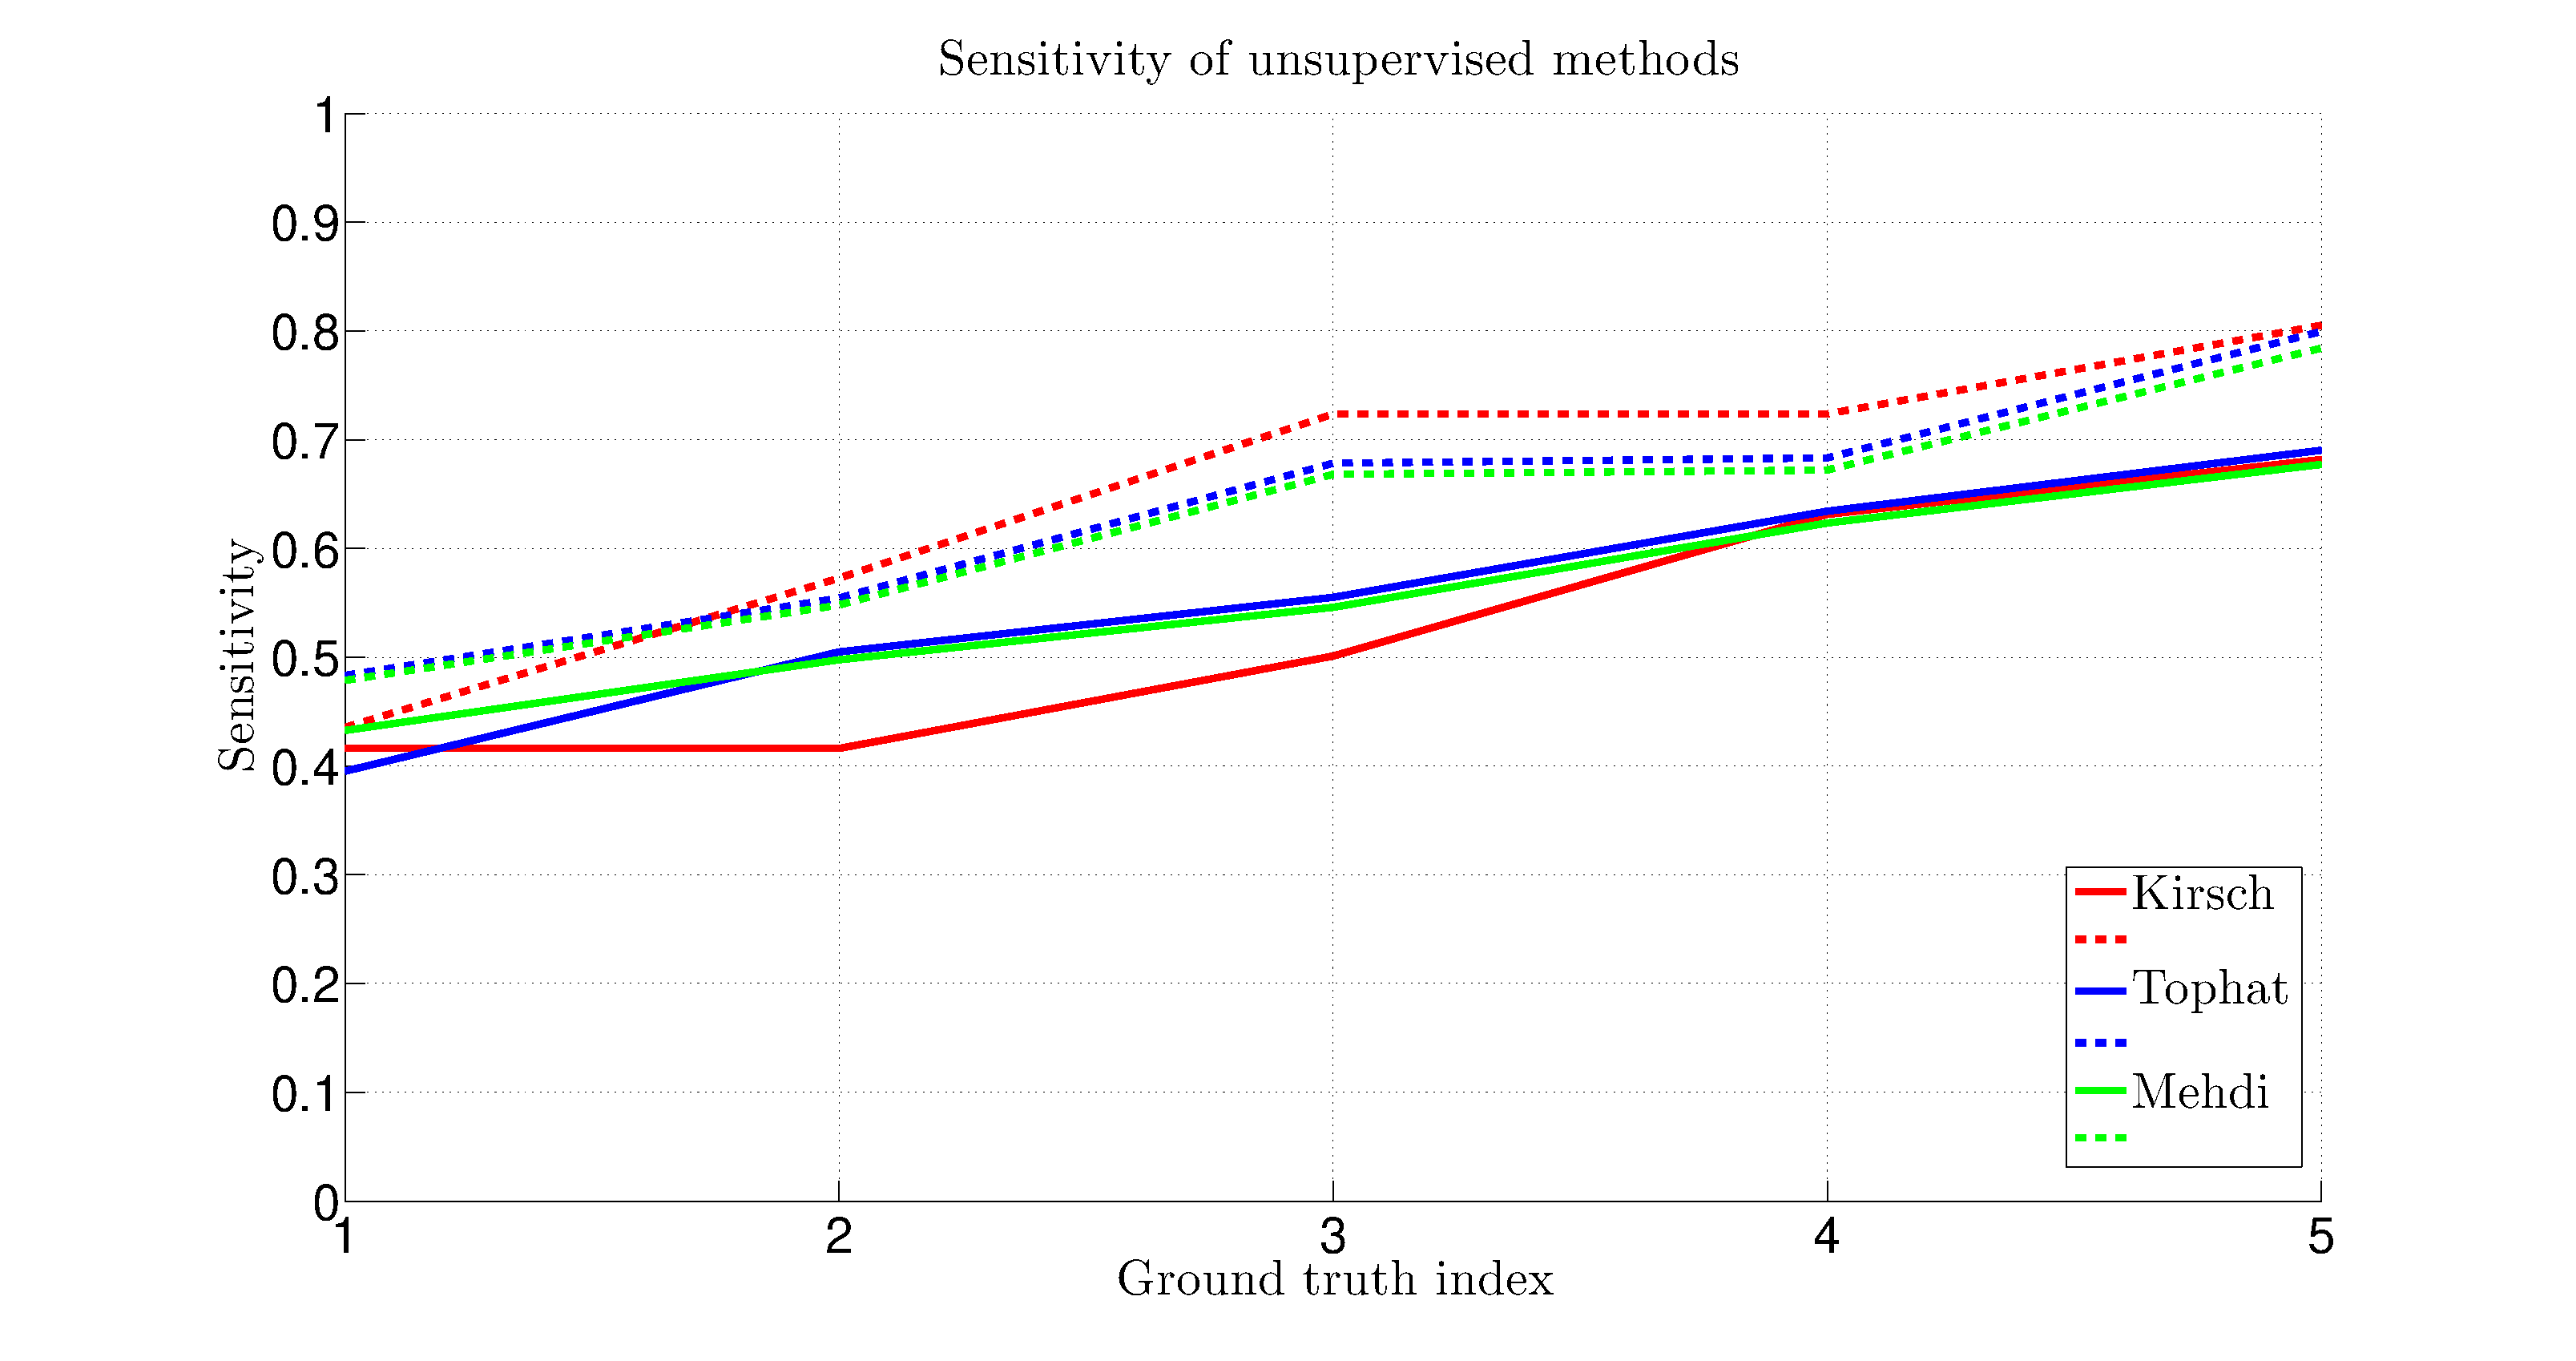
\includegraphics[width=0.95\textwidth]{hist_unsup_sens_imgset1}}

  \subfloat[]{
     \label{fig:unsupspec}
     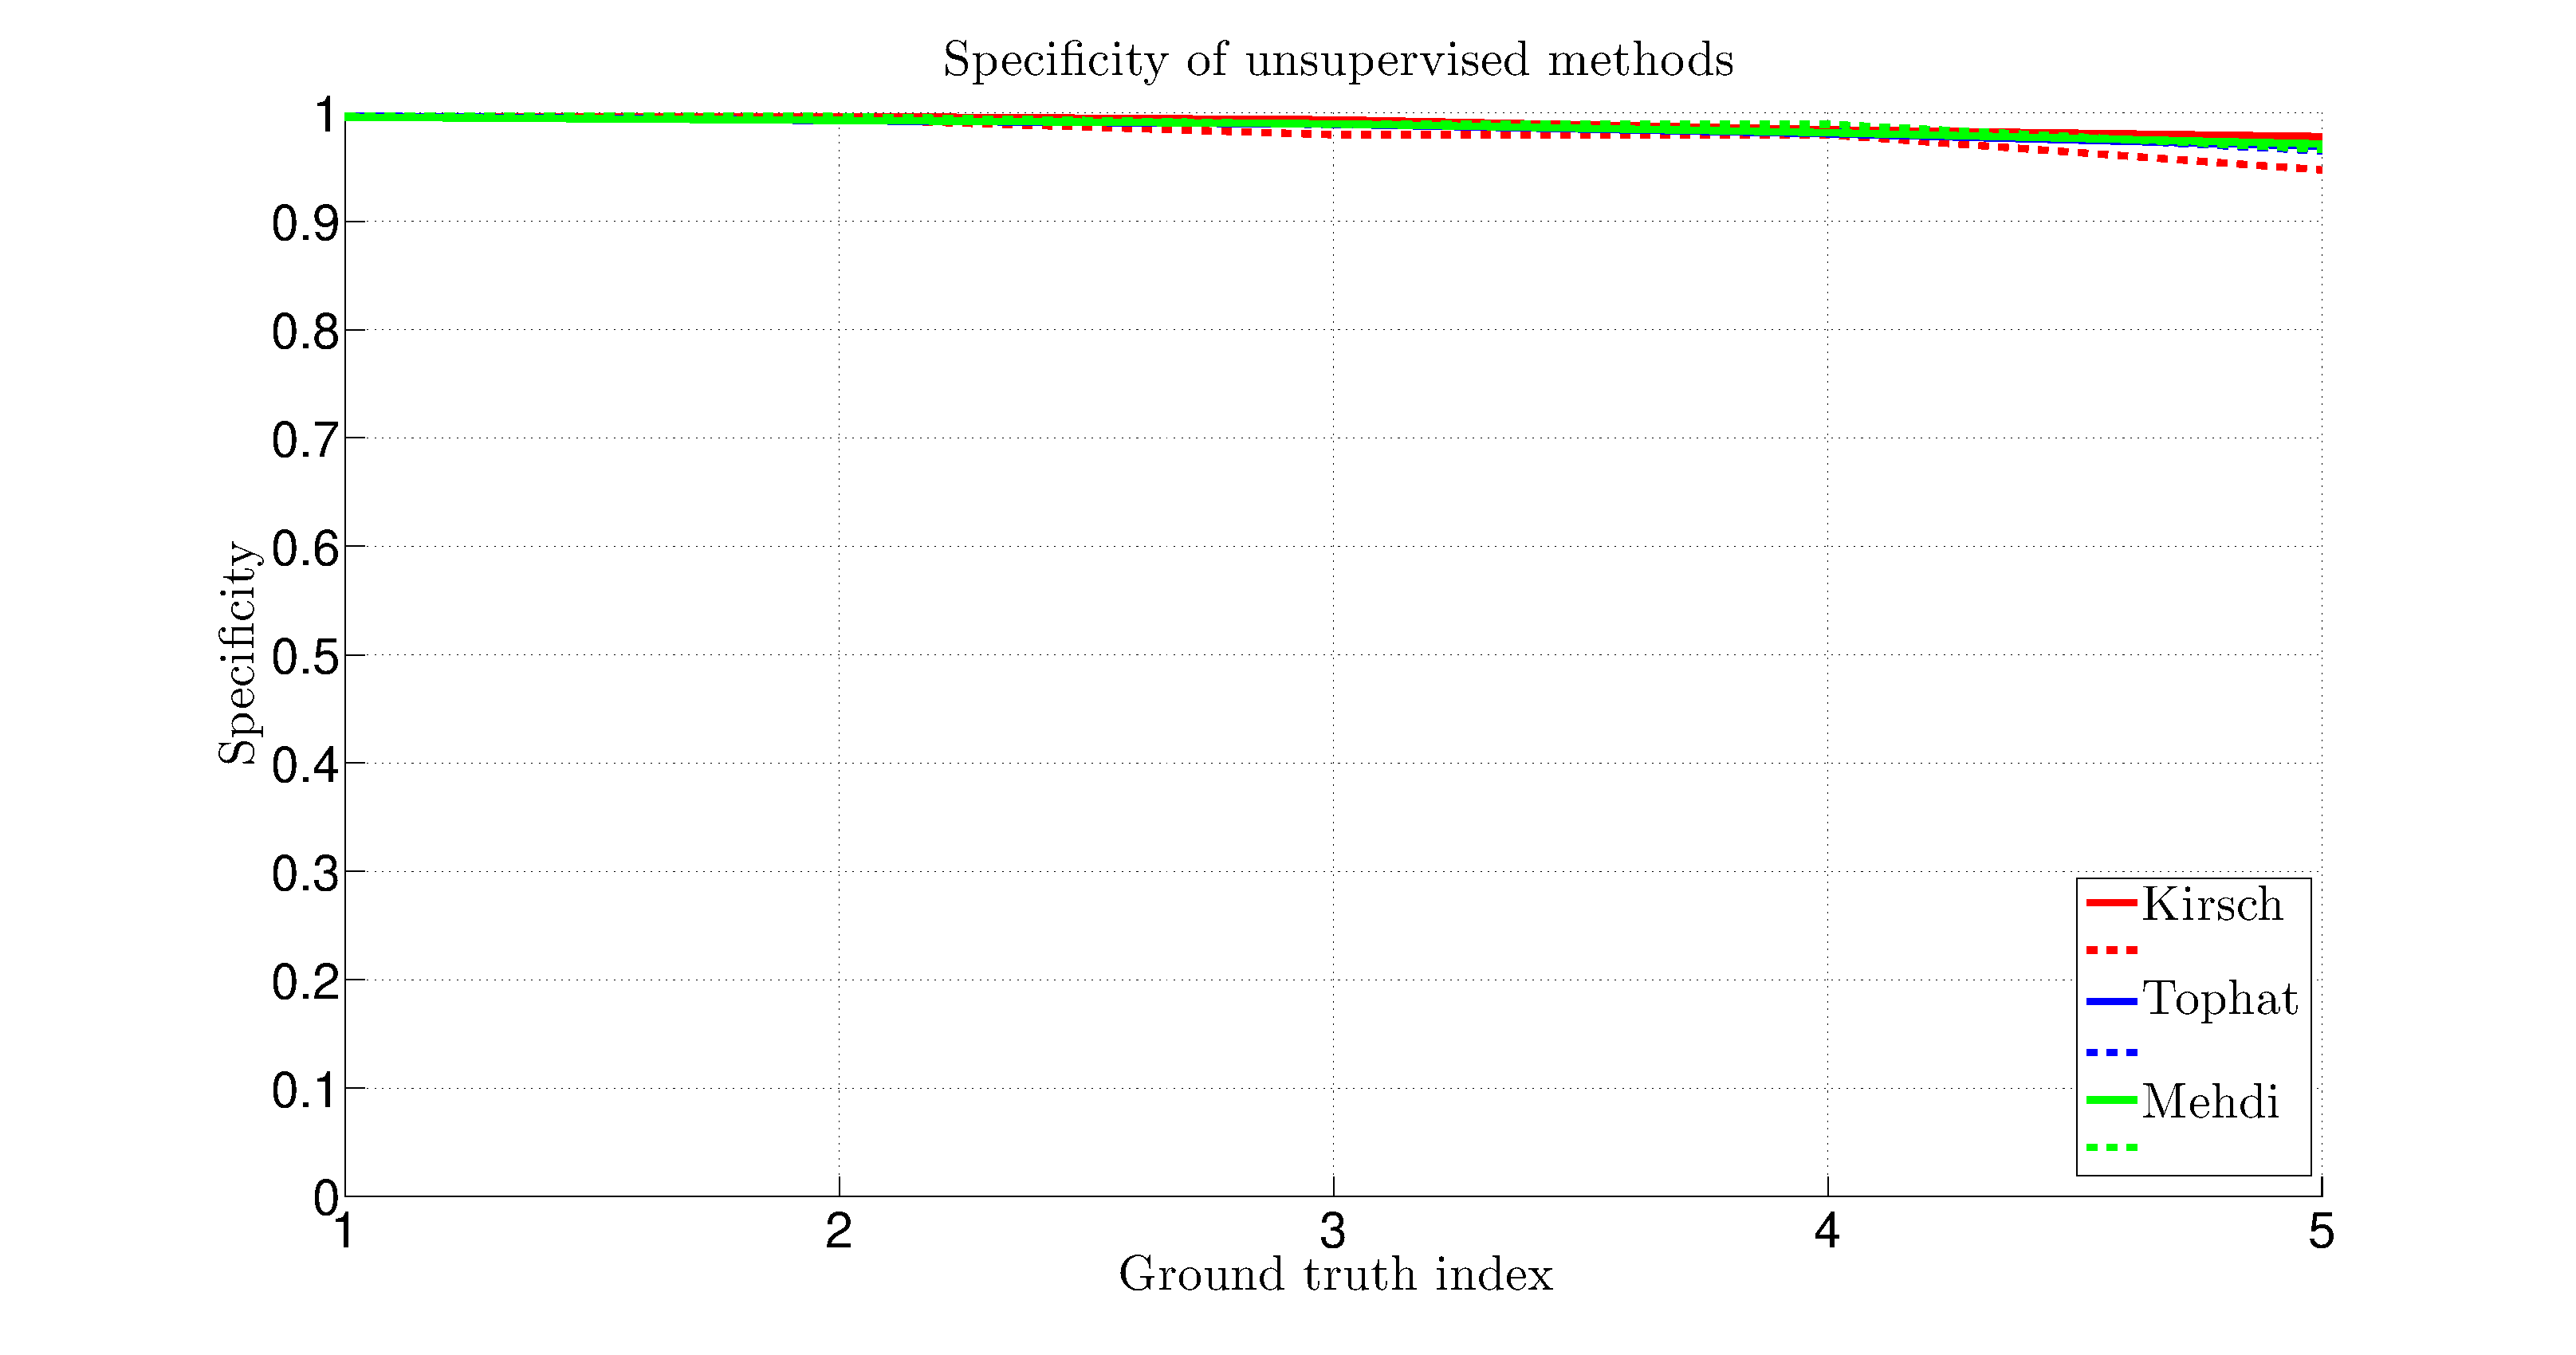
\includegraphics[width=0.95\textwidth]{hist_unsup_spec_imgset1}}
     
  \caption[moving]{Performance of unsupervised methods:
  \subref{fig:unsupsens} Sensitivity
  \subref{fig:unsupspec} Specificity. Note that these graphs represent
  the methods' performance over images that have exudates present. The original
  Bristol ground truth is on the left on the x-axis, and the most inaccurate
  ground truth is on the right. Solid and dotted lines represent the use of different
  training/testing sets, as described in Section~\ref{subsubsec:settings}. }
  \label{fig:unsup}

}\end{figure}

\section{DISCUSSION}
\label{sec:discussion}

The main goal of this thesis was to study if and how much the spatial accuracy of the ground truth affects
the segmentation of retinal images using different image features and segmentation methods. Two supervised methods
were compared, Na�ve-Bayes and GMM-Bayes. Classifiers were trained with color, edge and texture features.
The performance of unsupervised edge detection methods was also evaluated.

The segmentation results of all used methods confirm the fact that accuracy of the used ground truth has a significant
impact on the segmentation performance. As for the features, classifiers using the edge feature outperformed color and texture
based classifiers. Even though texture seemed promising in initial testing, texture-based classifiers were unable to
even partially find exudates from the images.

GMM-Bayes was expected to outperform the simpler Na�ve-Bayes, but there was no clear difference in overall performance of these methods.
However, Na�ve-Bayes' performance with higher levels of inaccuracy in the ground truth was much more predictable, as the segmentation 
accuracy declined almost linearly as the ground truth became more inaccurate. The performance of GMM-Bayes classifiers, mainly the ones
using texture, was less linear. The performance of unsupervised edge detection methods was significantly better than the performance
of Na�ve- and GMM-Bayes, largely due to the mask used to exclude the blood vessels. 

The second goal of the thesis was to evaluate the performance of features other than color. Based on the performance of 
the unsupervised methods and edge-based classifiers of supervised methods, using the edge feature in exudate segmentation proves to be a 
valid method. Future work is required in studying the usefulness of texture in this matter.


% Bibliography
%% This must be here, not in preamble, if you want it to work
\addcontentsline{toc}{section}{REFERENCES}
\bibliography{resources/thesis}

%% ----------------------- APPENDICES ------------------------------

\appendix

\section{Example results of unsupervised methods}
\label{app:unsupervised}

\begin{minipage}[c]{\textwidth}
  \label{fig:eye34_kirsch}
  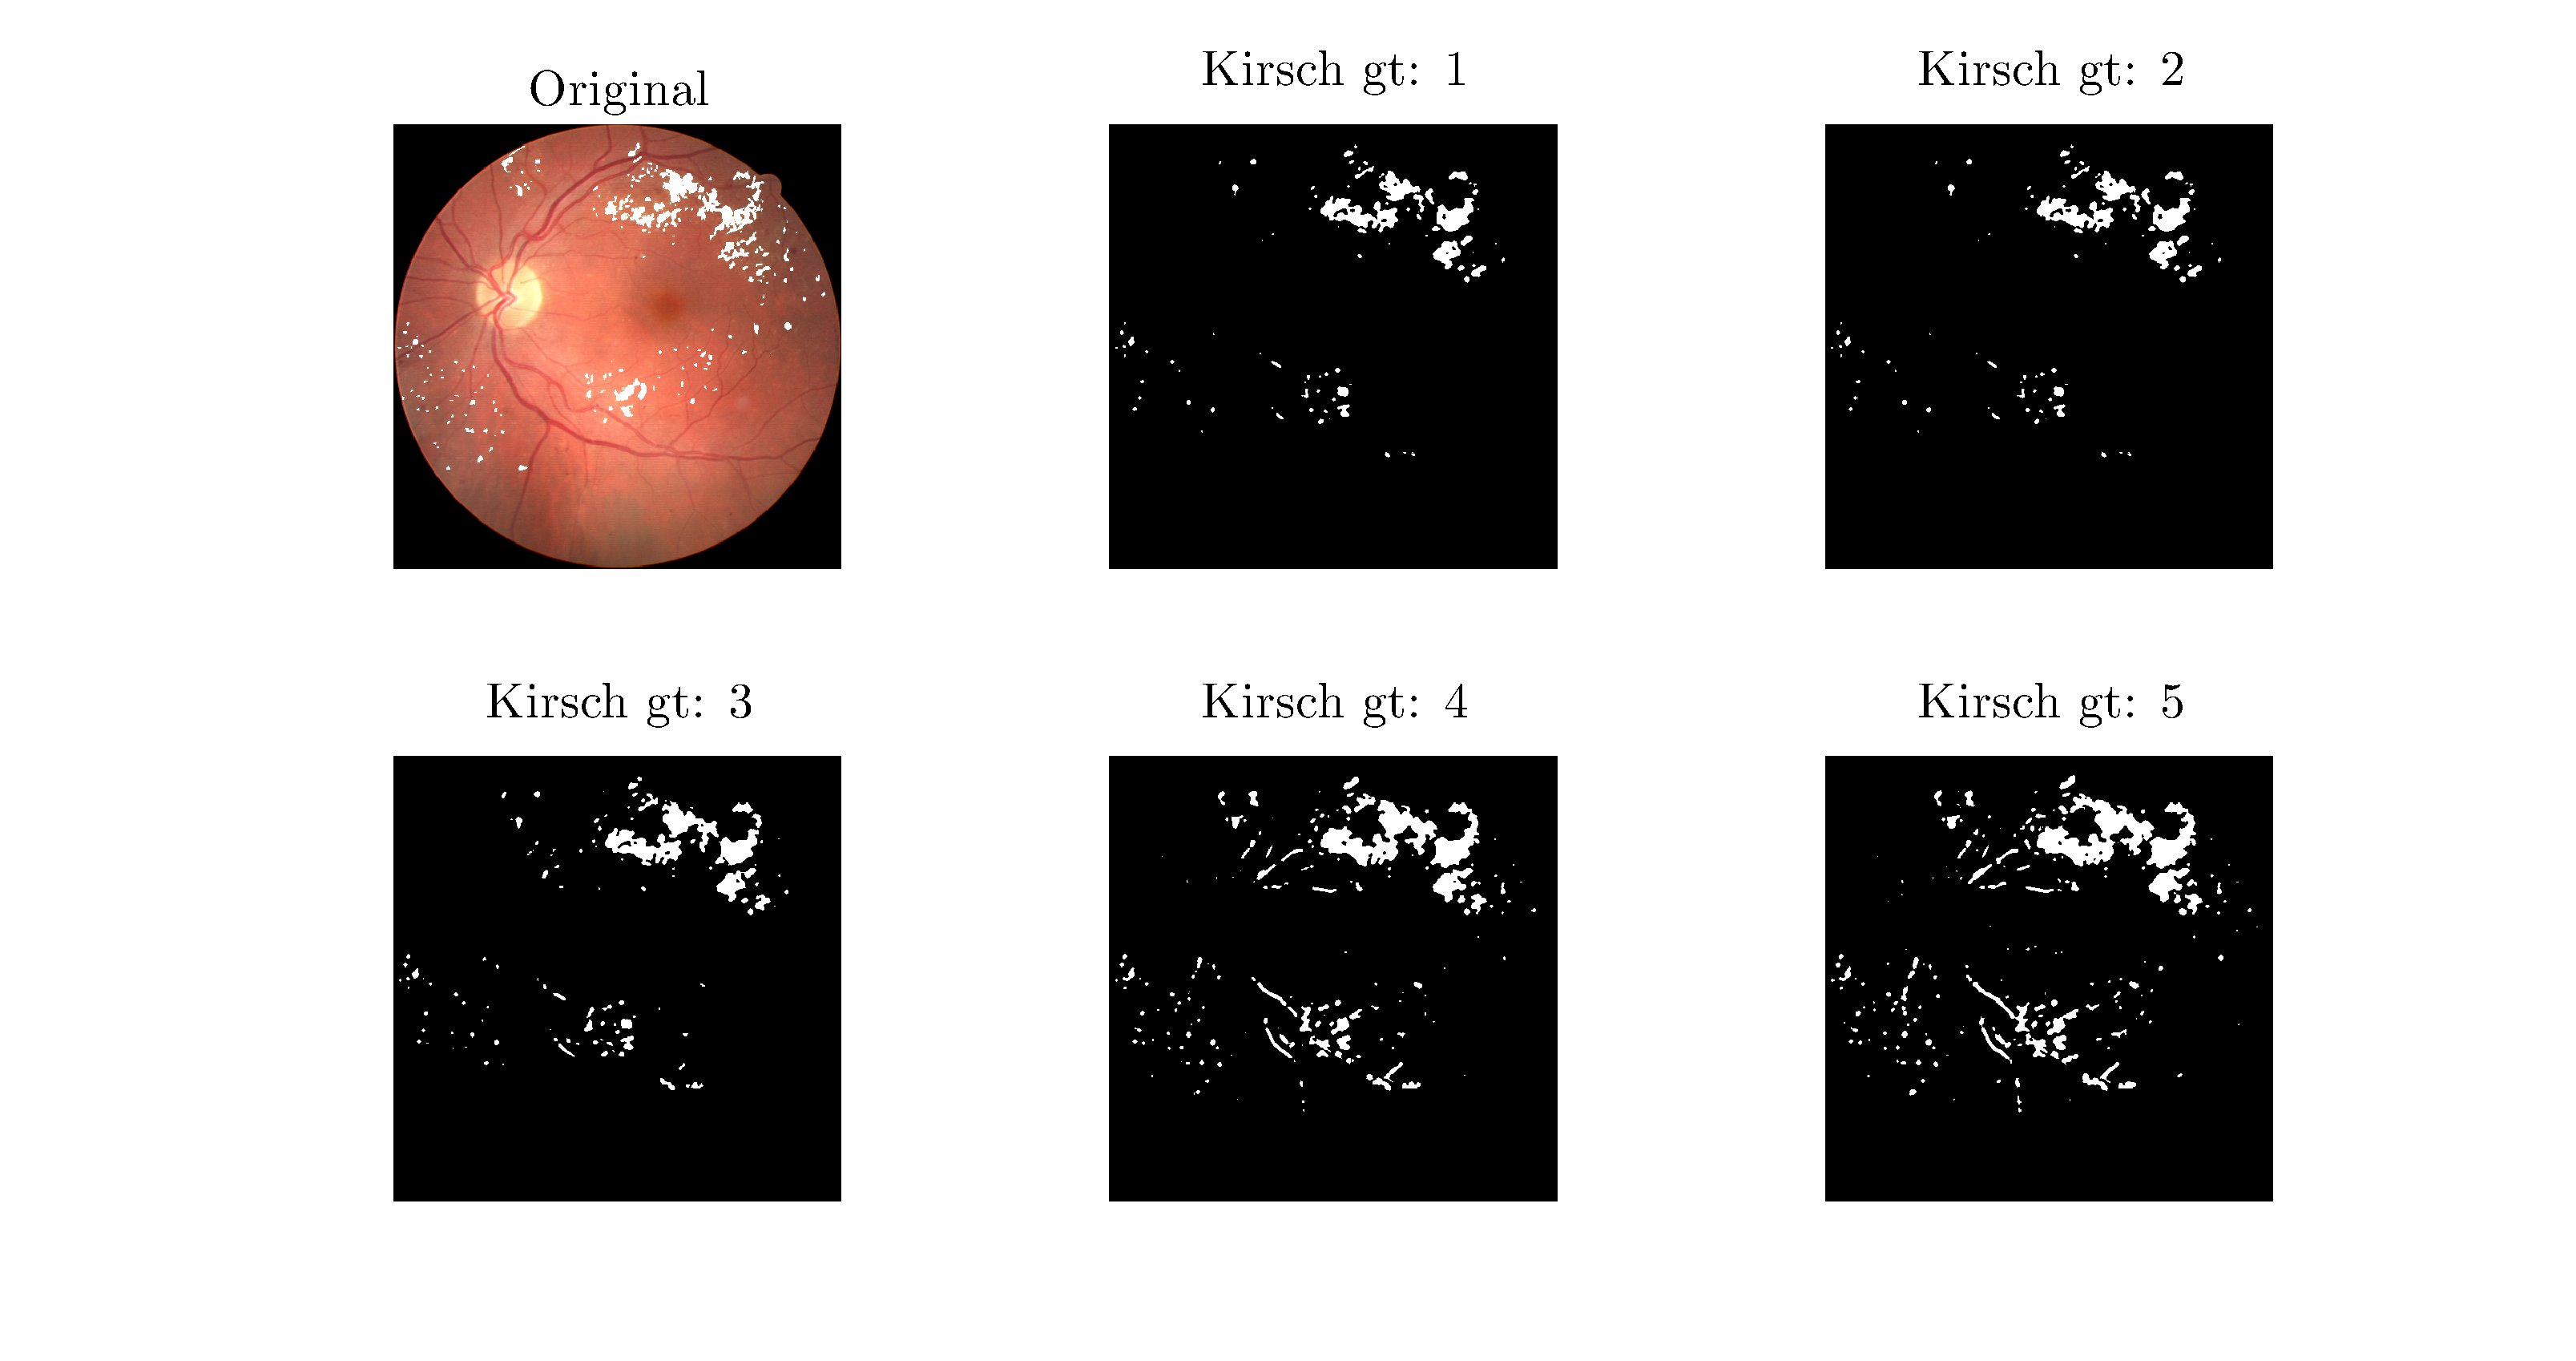
\includegraphics[width=1.4\textwidth,angle=90]{eye_kirsch_34}     
  \captionof{figure}{Example results of Kirsch. The original ground truth is shown superimposed on the image of the eye fundus.
  The segmentation results of the method are shown as a binary image. The results with the accurate ground truth are shown first (1), then the results
  with the three iterations of inaccurate ground truth (2-4), and lastly the results with the most inaccurate ground truth (5).}
\end{minipage}

\begin{minipage}[c]{\textwidth}
  \label{fig:eye34_tophat}
  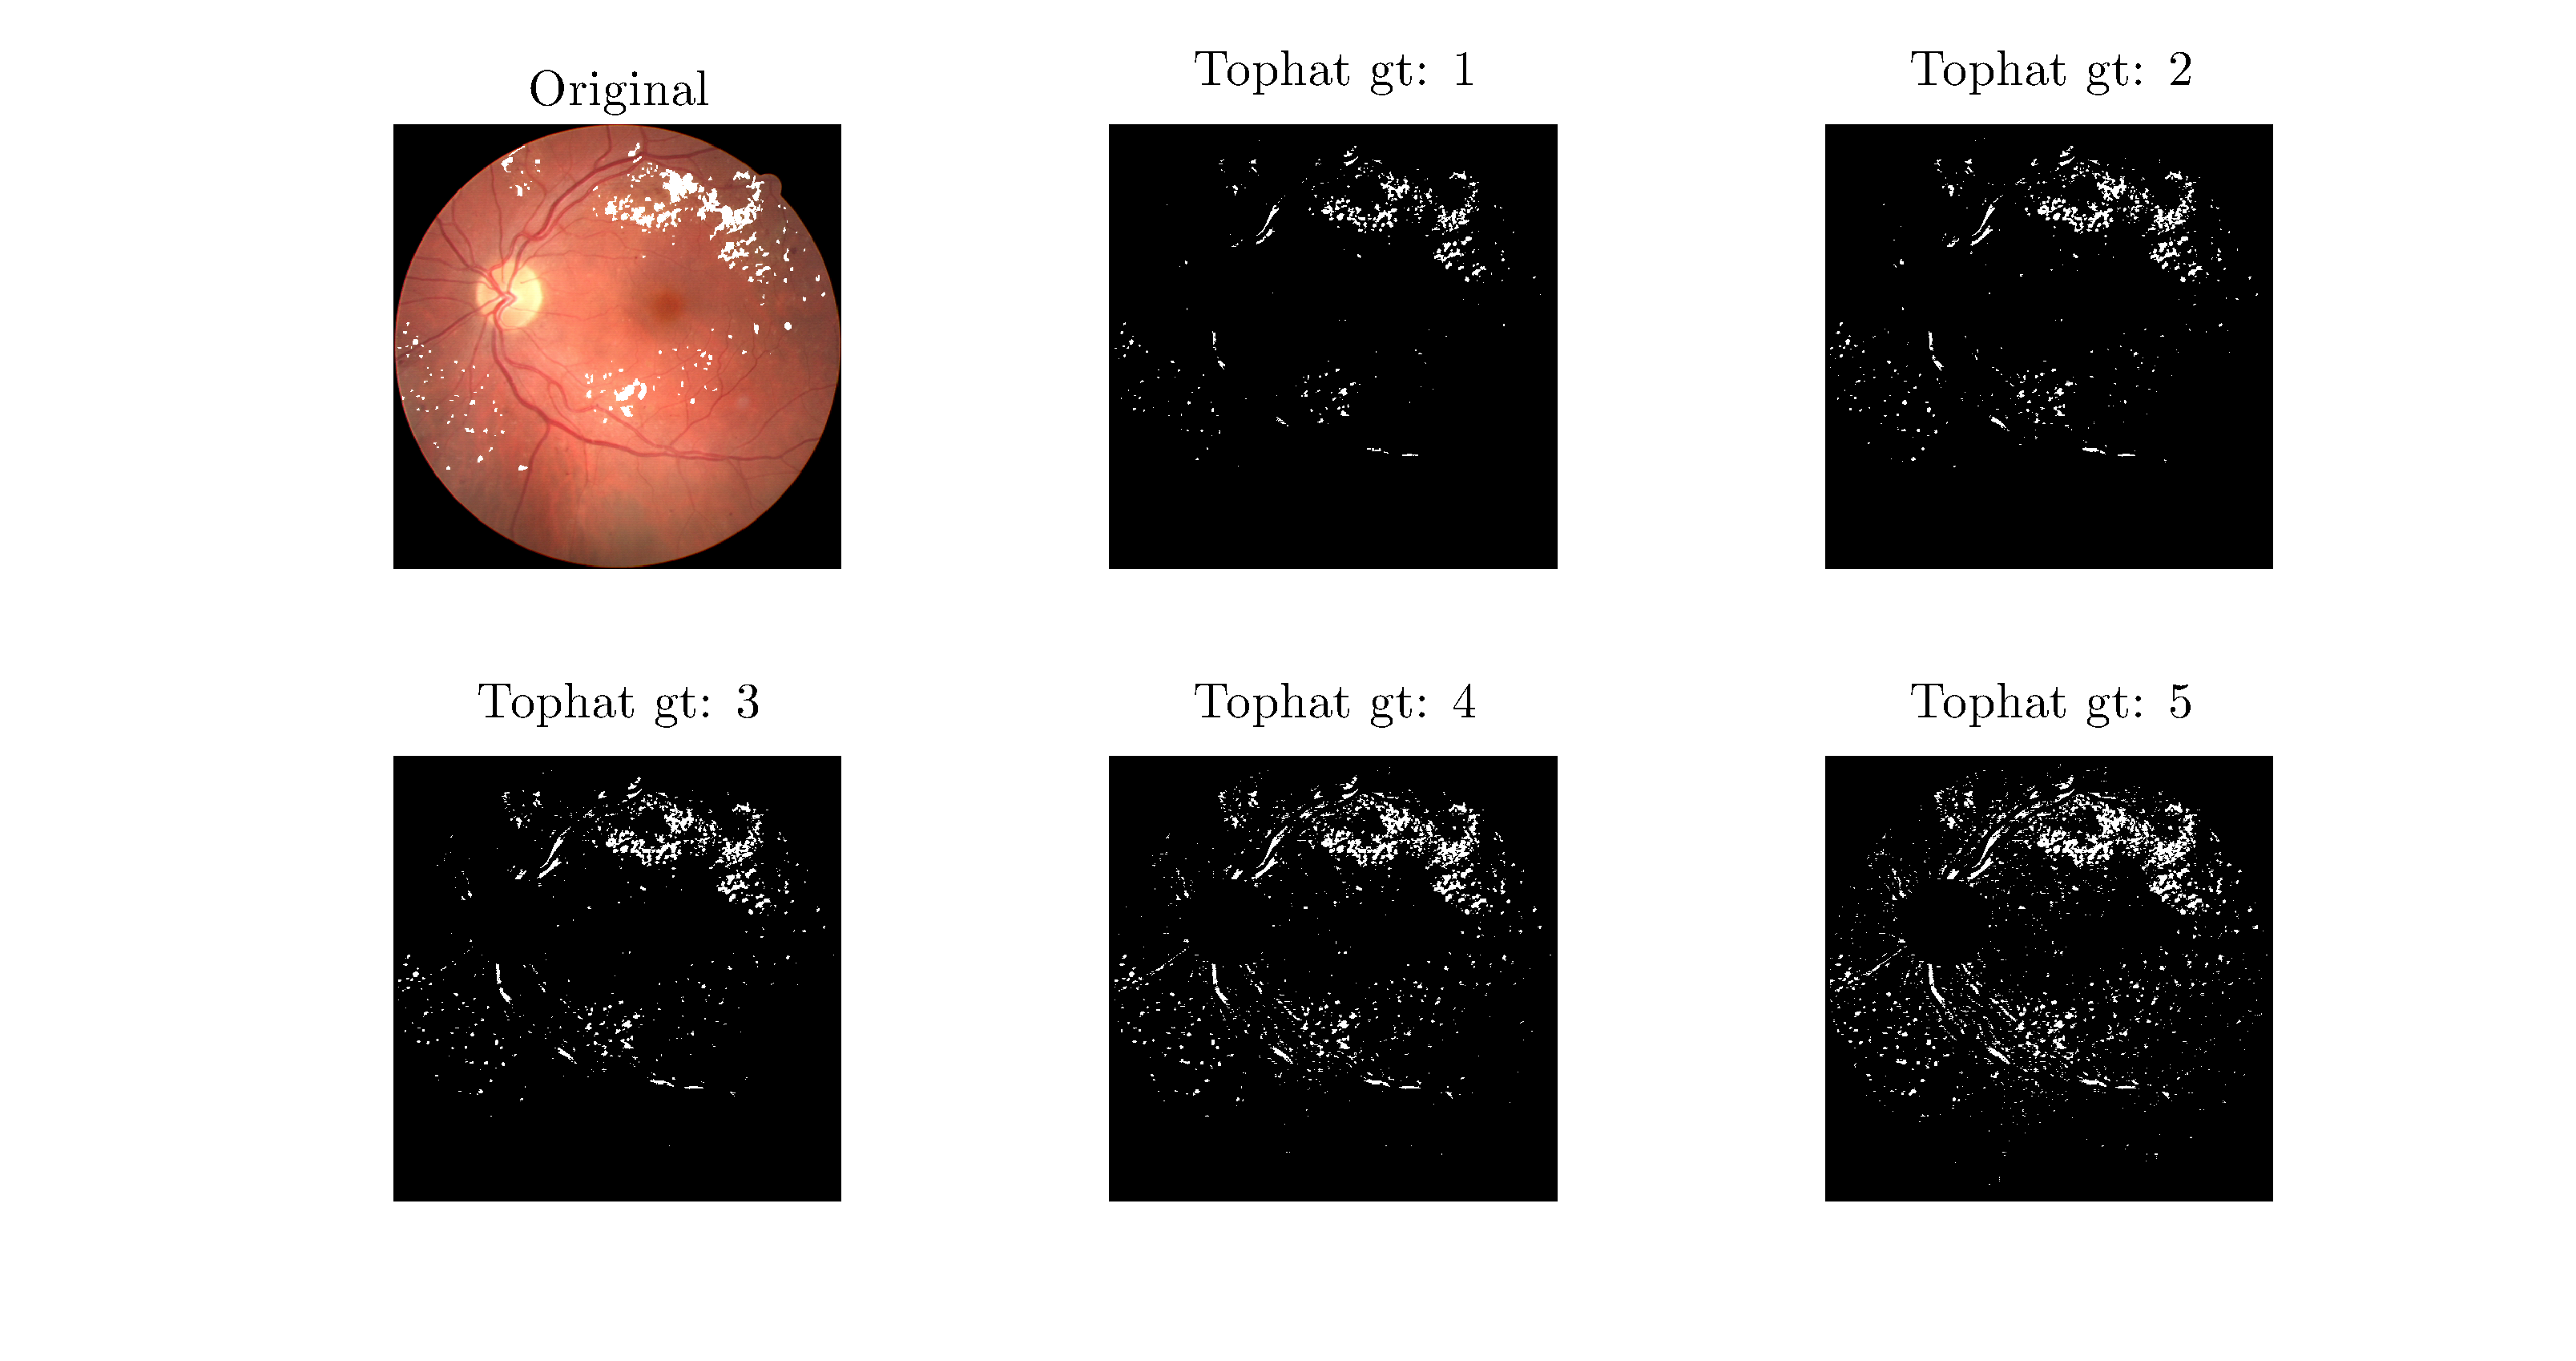
\includegraphics[width=1.4\textwidth,angle=90]{eye_tophat_34}     
  \captionof{figure}{Example results of Tophat. The original ground truth is shown superimposed on the image of the eye fundus.
  The segmentation results of the method are shown as a binary image. The results with the accurate ground truth are shown first (1), then the results
  with the three iterations of inaccurate ground truth (2-4), and lastly the results with the most inaccurate ground truth (5).}
\end{minipage}

\sectionend

\section{Example results of Na�ve-Bayes}
\label{app:bayes}


\begin{minipage}[c]{\textwidth}
  \label{fig:eye28_bayes_color}
  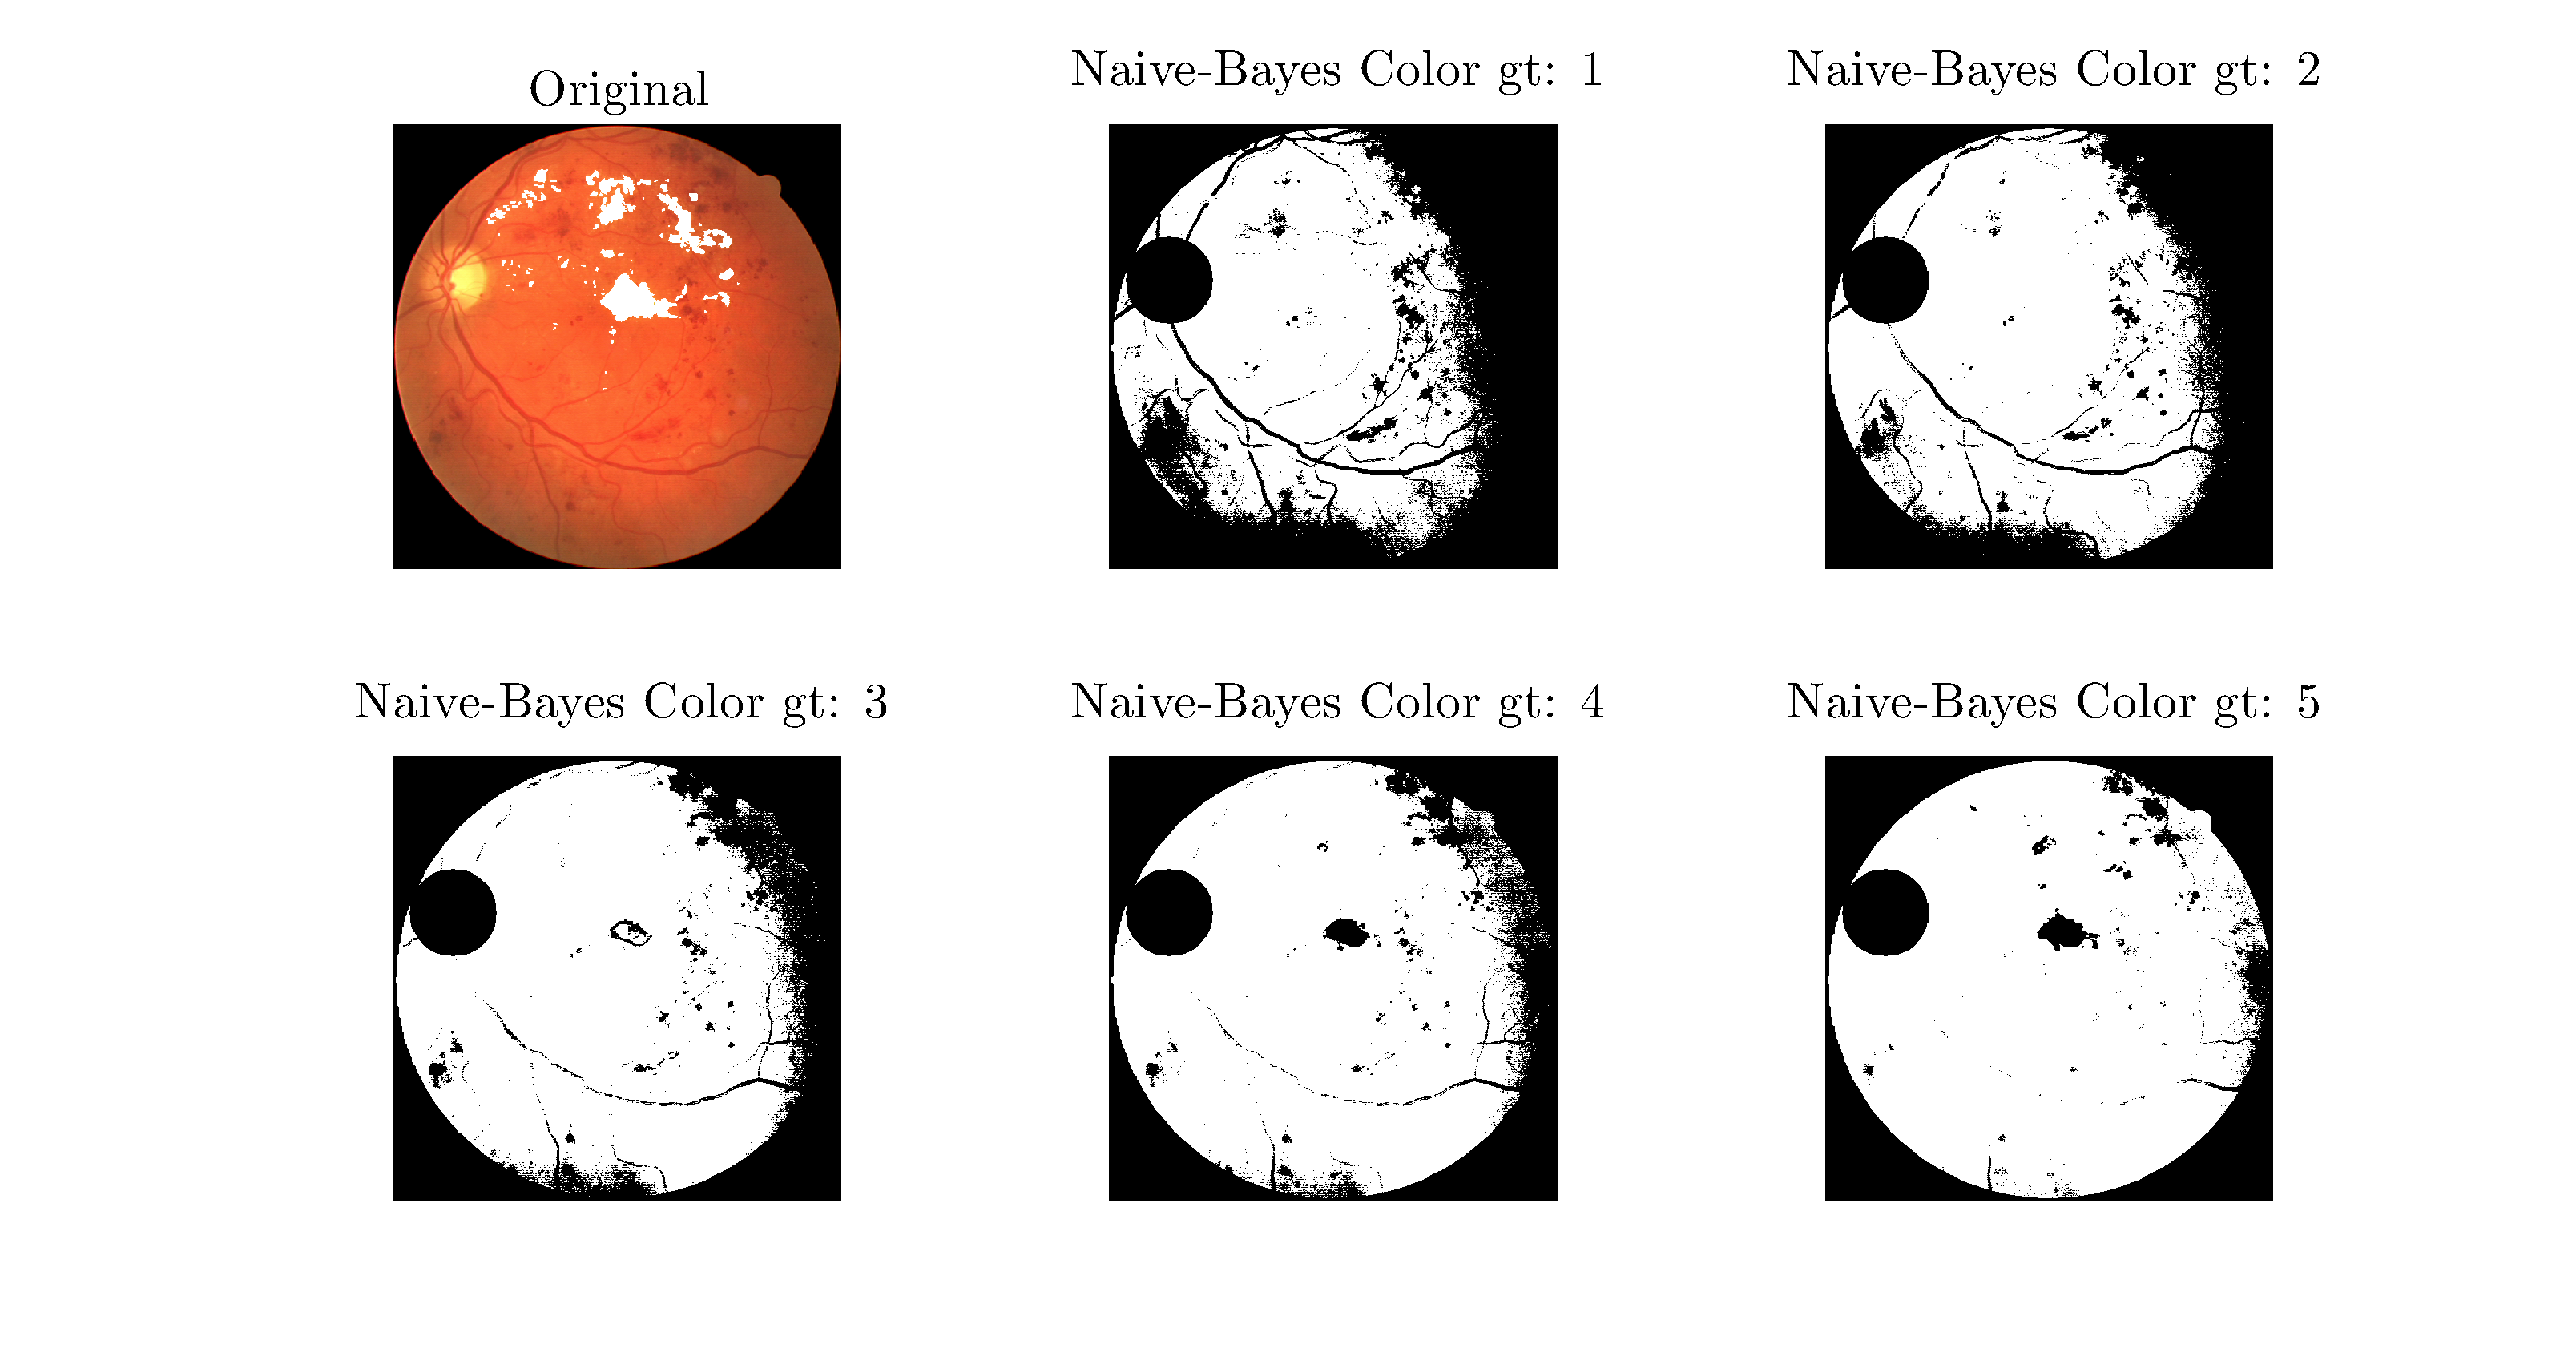
\includegraphics[width=1.4\textwidth,angle=90]{eye_bayes_color_28}     
  \captionof{figure}{Example results of Na�ve-Bayes classifier using color. The original ground truth is shown superimposed on the image of the eye fundus.
  The segmentation results of the method are shown as a binary image. The results with the accurate ground truth are shown first (1), then the results
  with the three iterations of inaccurate ground truth (2-4), and lastly the results with the most inaccurate ground truth (5).}
\end{minipage}

\begin{minipage}[c]{\textwidth}
    \label{fig:eye28_bayes_edge}
    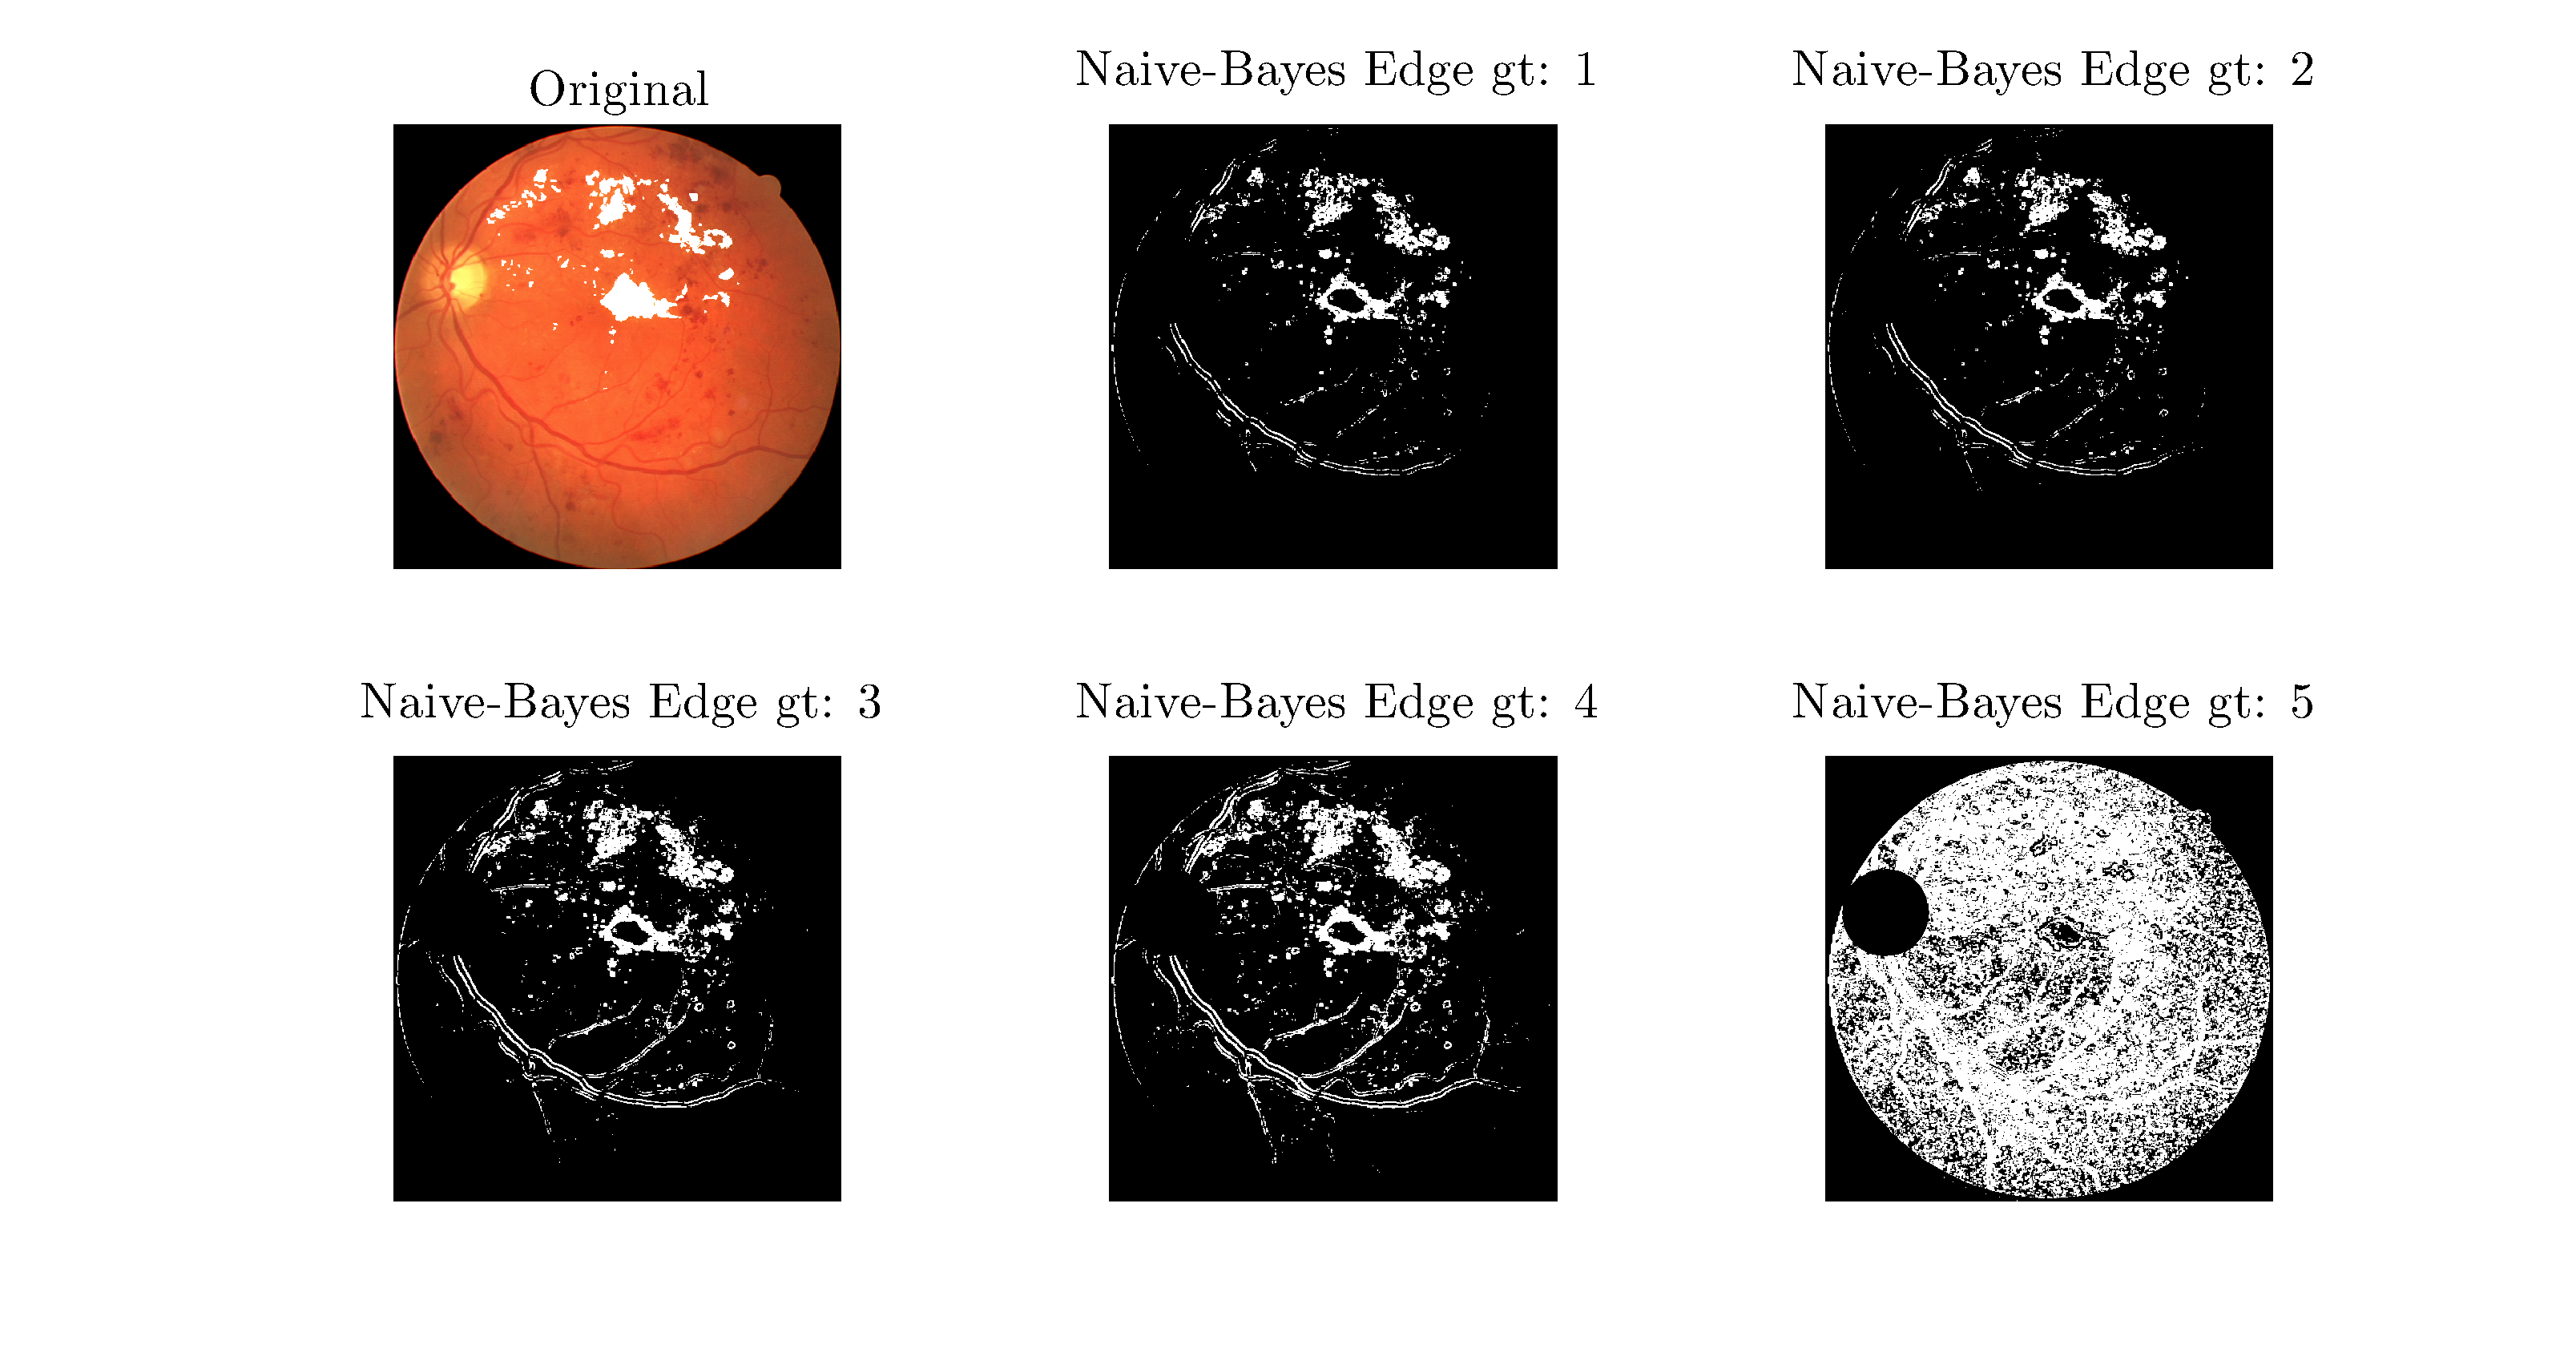
\includegraphics[width=1.4\textwidth,angle=90]{eye_bayes_edge_28}     
    \captionof{figure}{Example results of Na�ve-Bayes classifier using edge. The original ground truth is shown superimposed on the image of the eye fundus.
  The segmentation results of the method are shown as a binary image. The results with the accurate ground truth are shown first (1), then the results
  with the three iterations of inaccurate ground truth (2-4), and lastly the results with the most inaccurate ground truth (5).}

\end{minipage}

\begin{minipage}[c]{\textwidth}

    \label{fig:eye28_bayes_texture}
    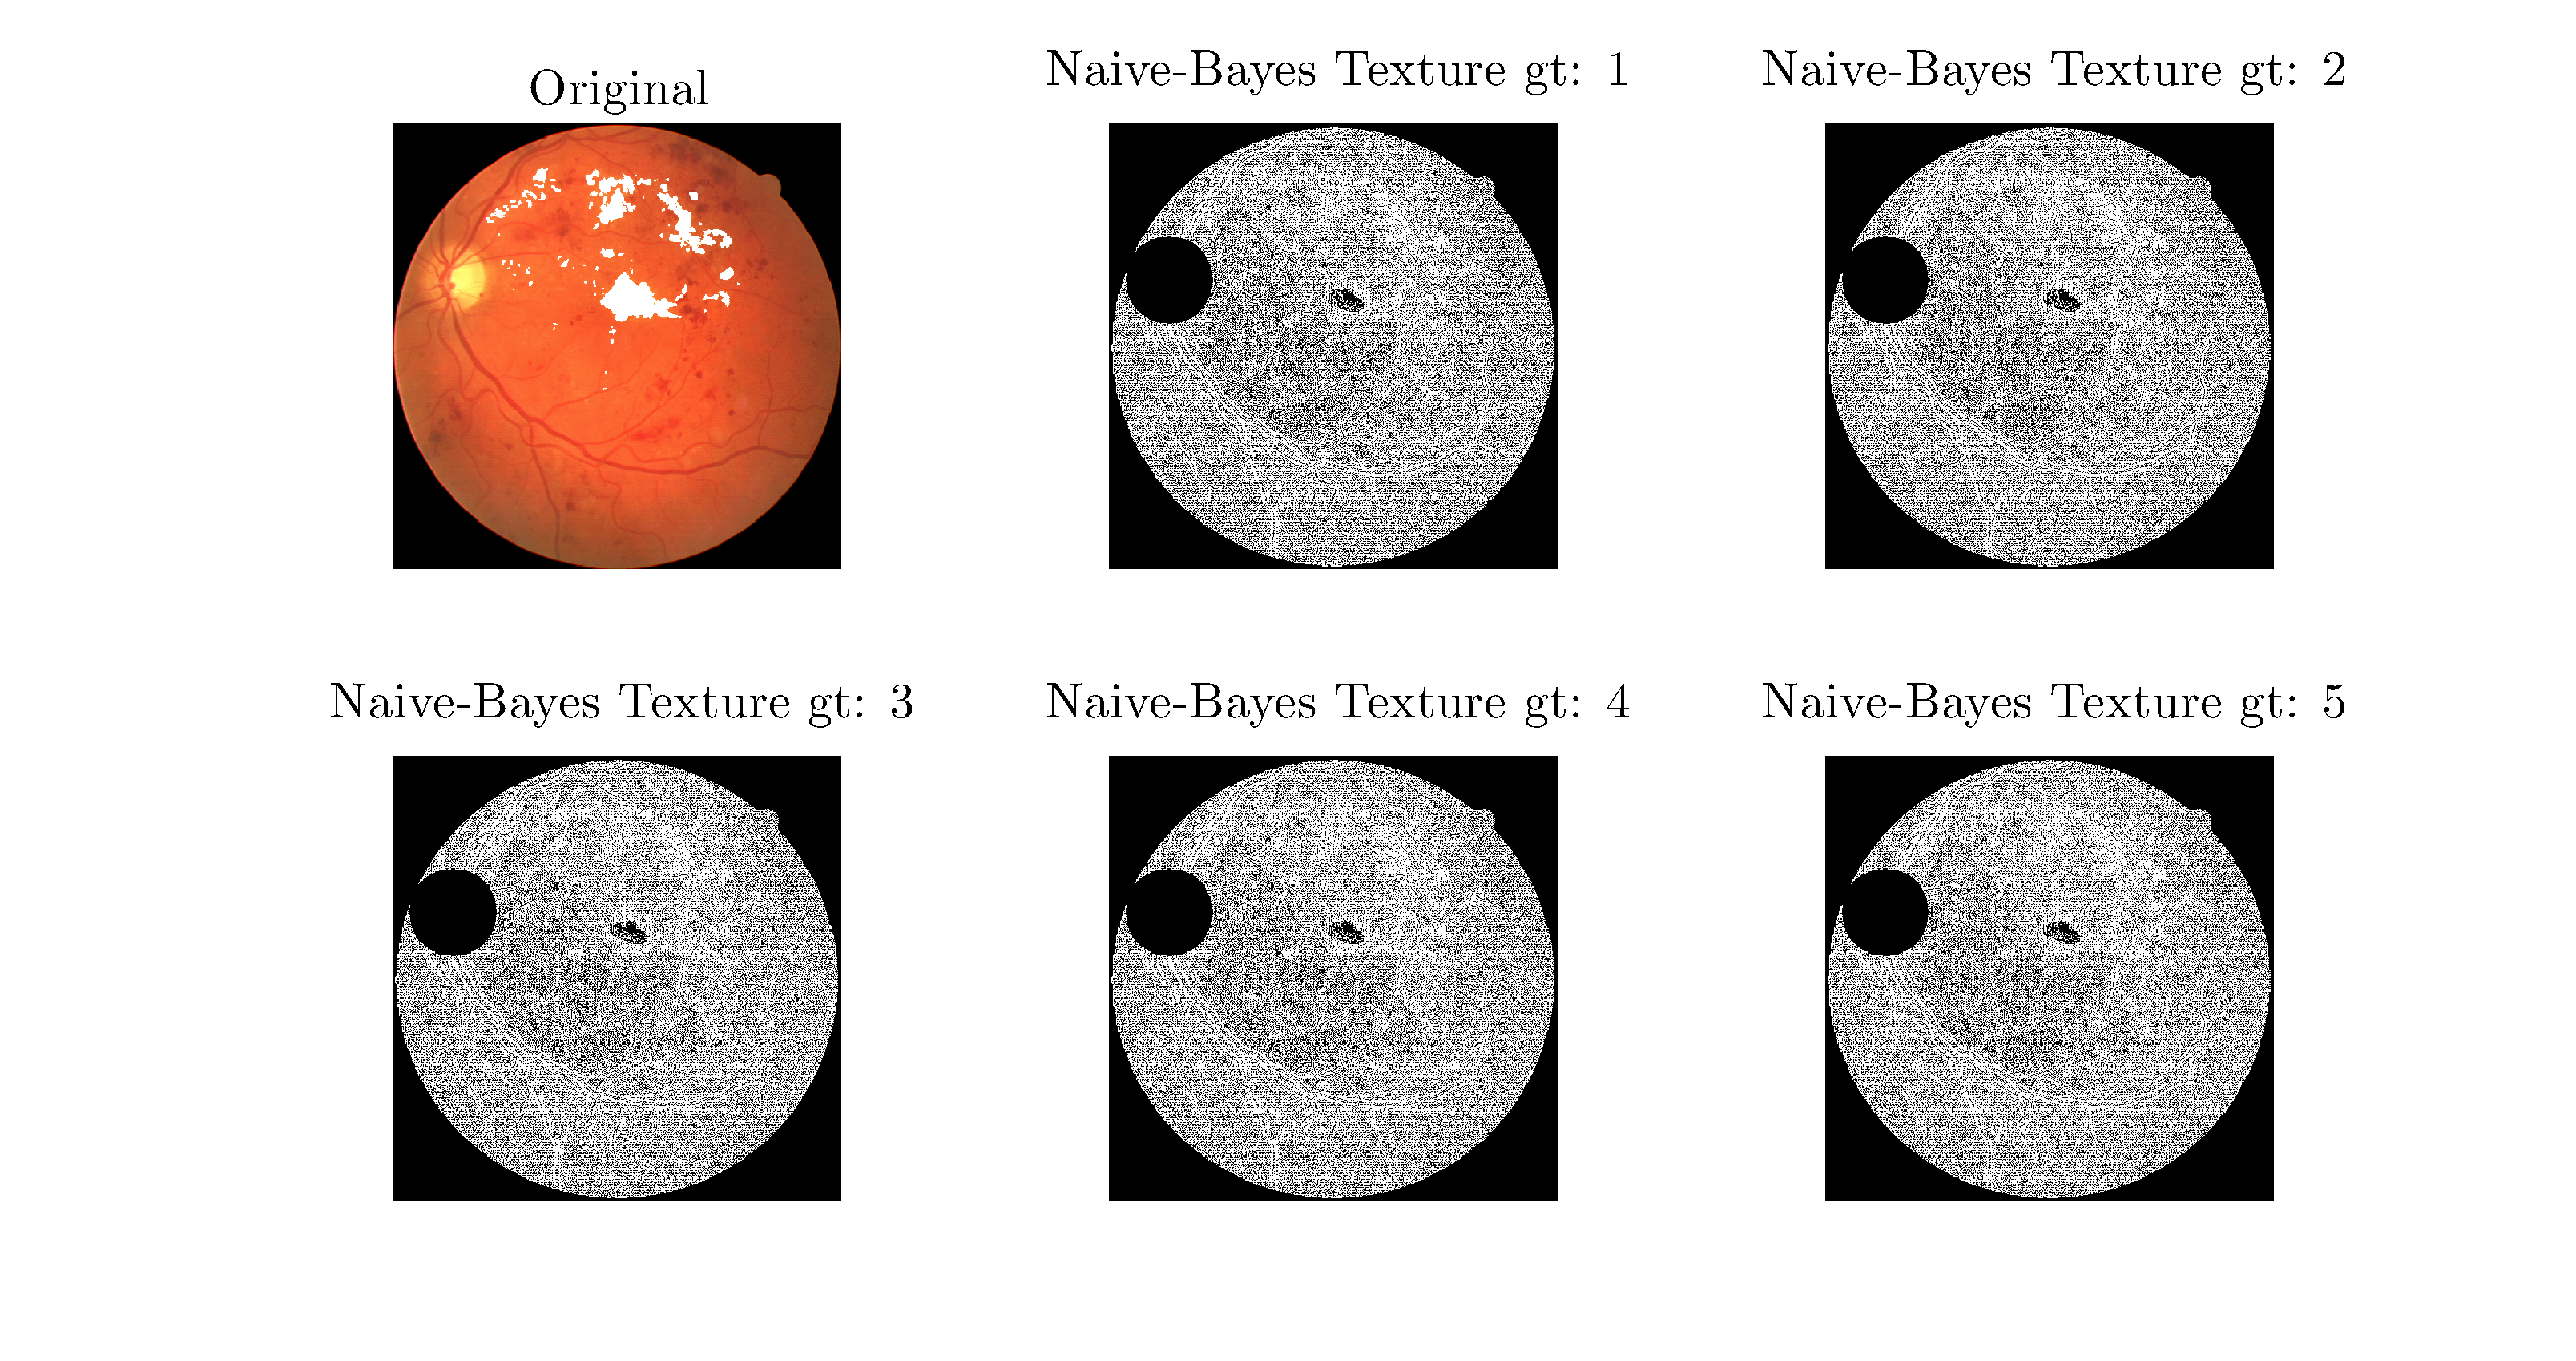
\includegraphics[width=1.4\textwidth,angle=90]{eye_bayes_texture_28}     
    \captionof{figure}{Example results of Na�ve-Bayes classifier using texture. The original ground truth is shown superimposed on the image of the eye fundus.
  The segmentation results of the method are shown as a binary image. The results with the accurate ground truth are shown first (1), then the results
  with the three iterations of inaccurate ground truth (2-4), and lastly the results with the most inaccurate ground truth (5).}

\end{minipage}

\begin{minipage}[c]{\textwidth}

    \label{fig:eye28_bayes_all}
    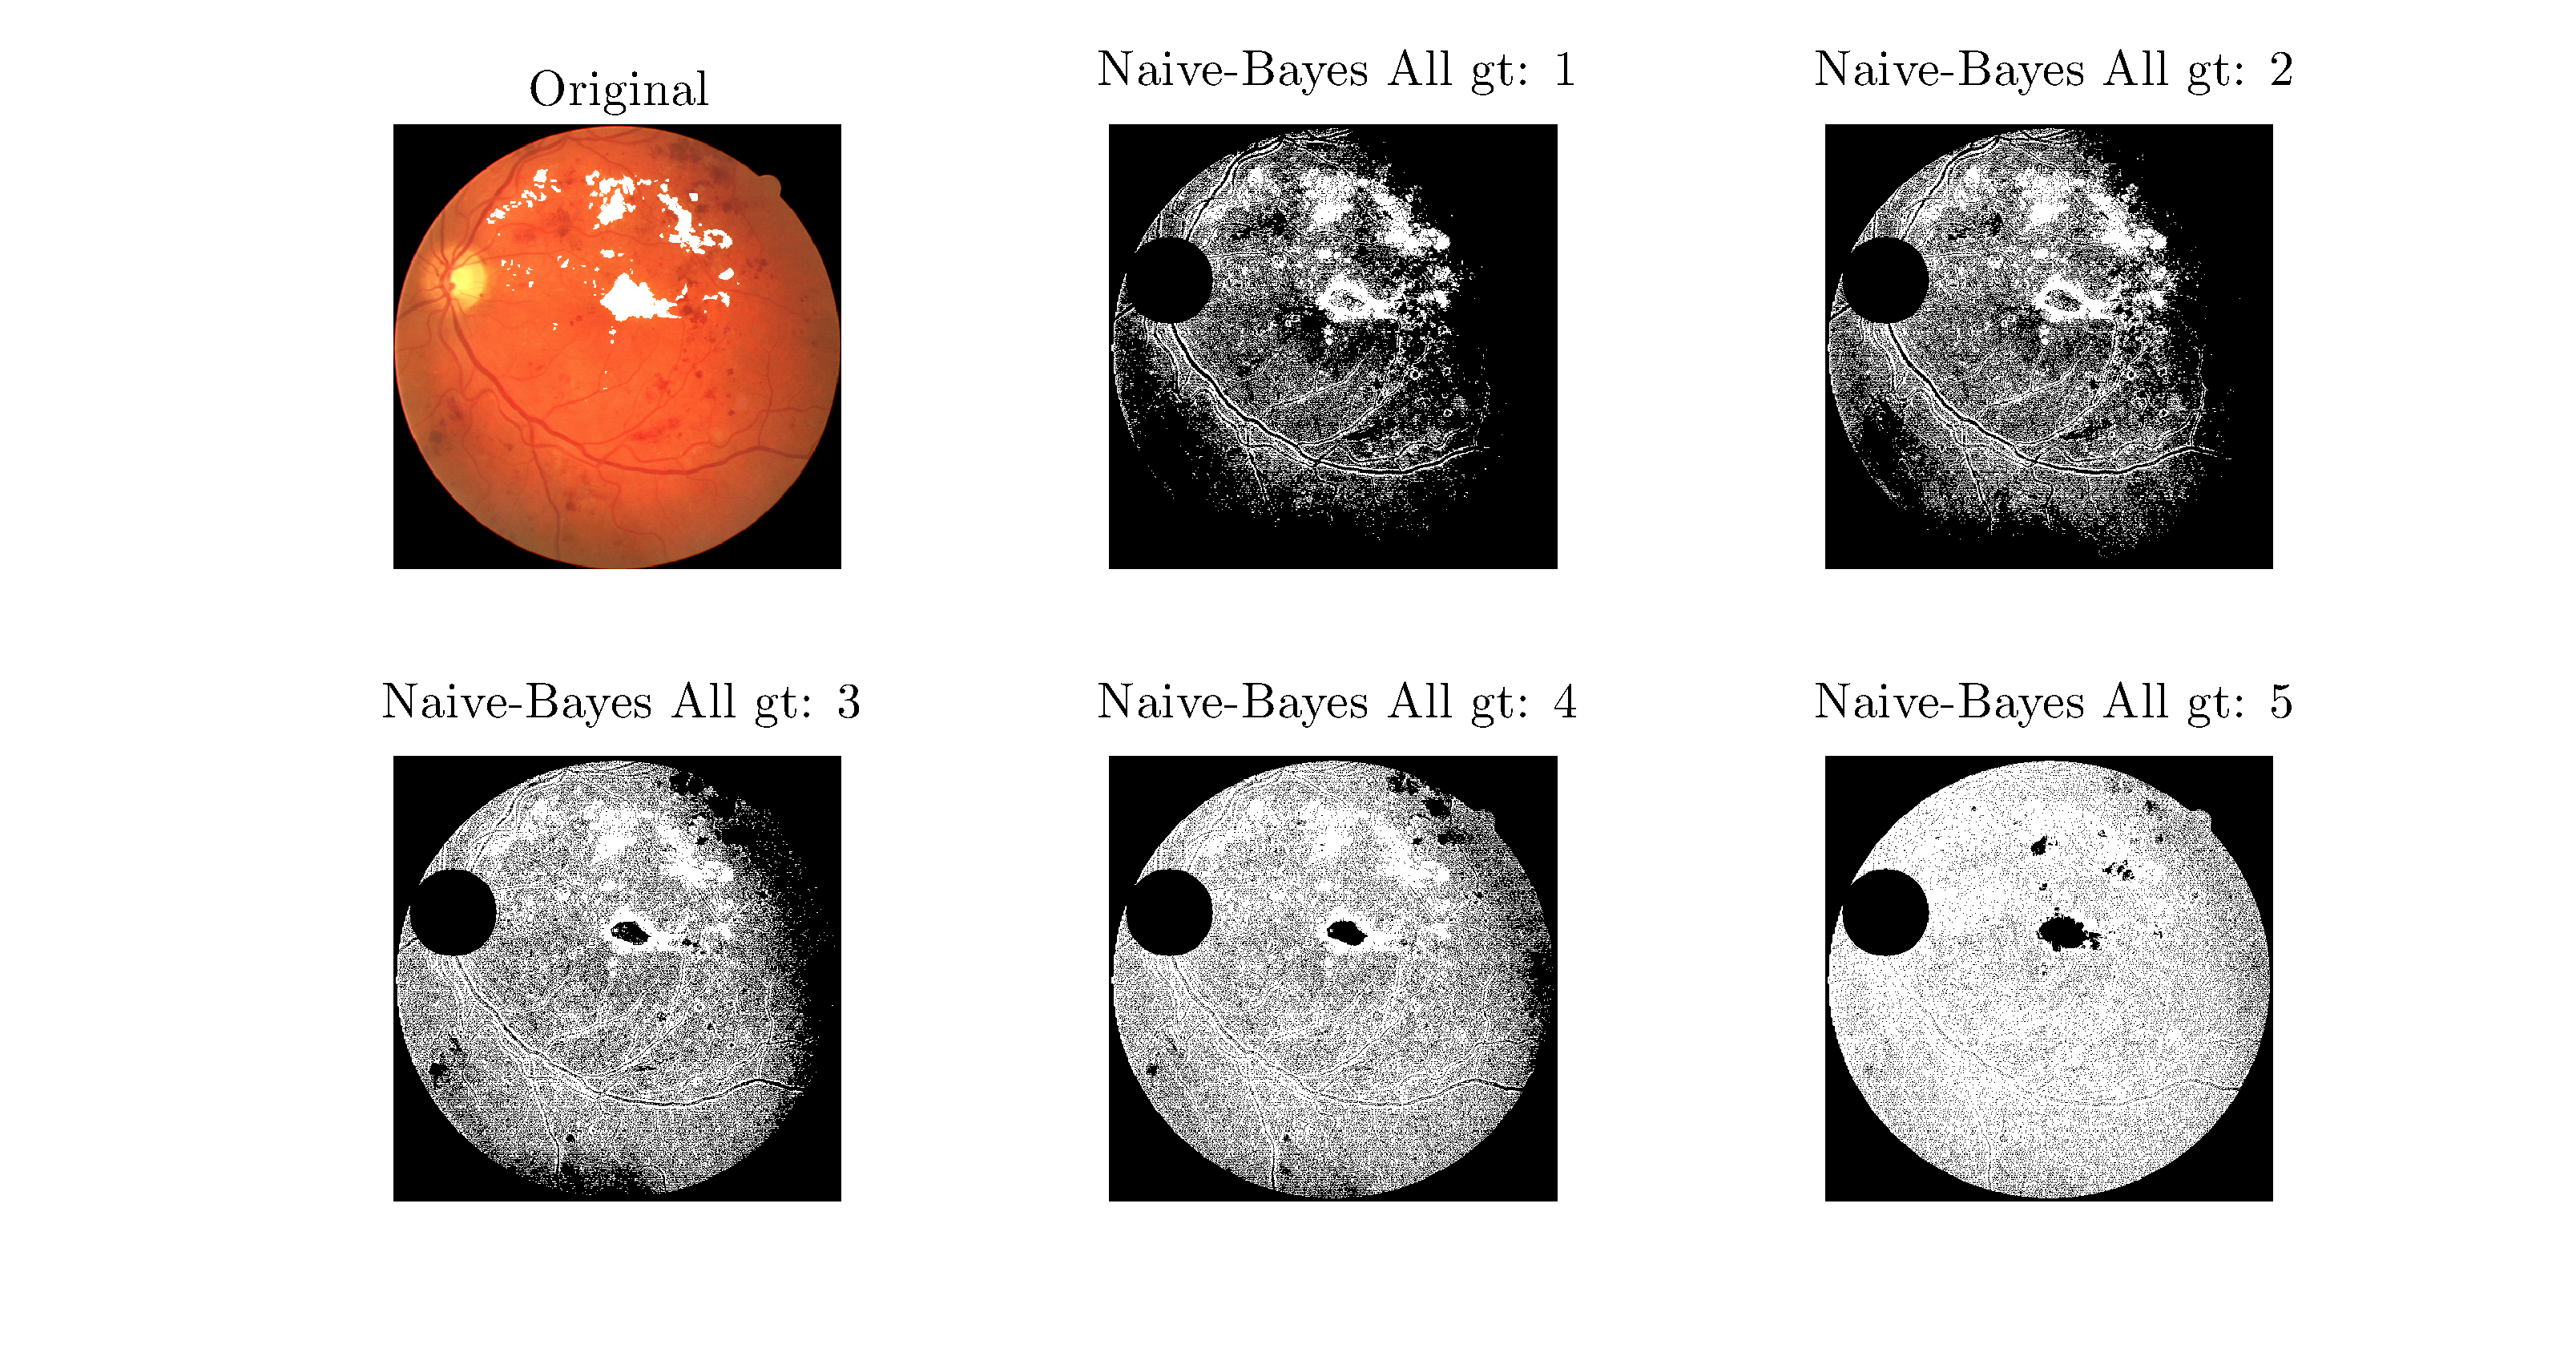
\includegraphics[width=1.4\textwidth,angle=90]{eye_bayes_all_28}     
    \captionof{figure}{Example results of Na�ve-Bayes classifier using all features. The original ground truth is shown superimposed on the image of the eye fundus.
  The segmentation results of the method are shown as a binary image. The results with the accurate ground truth are shown first (1), then the results
  with the three iterations of inaccurate ground truth (2-4), and lastly the results with the most inaccurate ground truth (5).}

\end{minipage}

\sectionend


\section{Example results of GMM-Bayes}
\label{app:gmmbayes}
\begin{minipage}[c]{\textwidth}

    \label{fig:eye28_gmmbayes_color}
    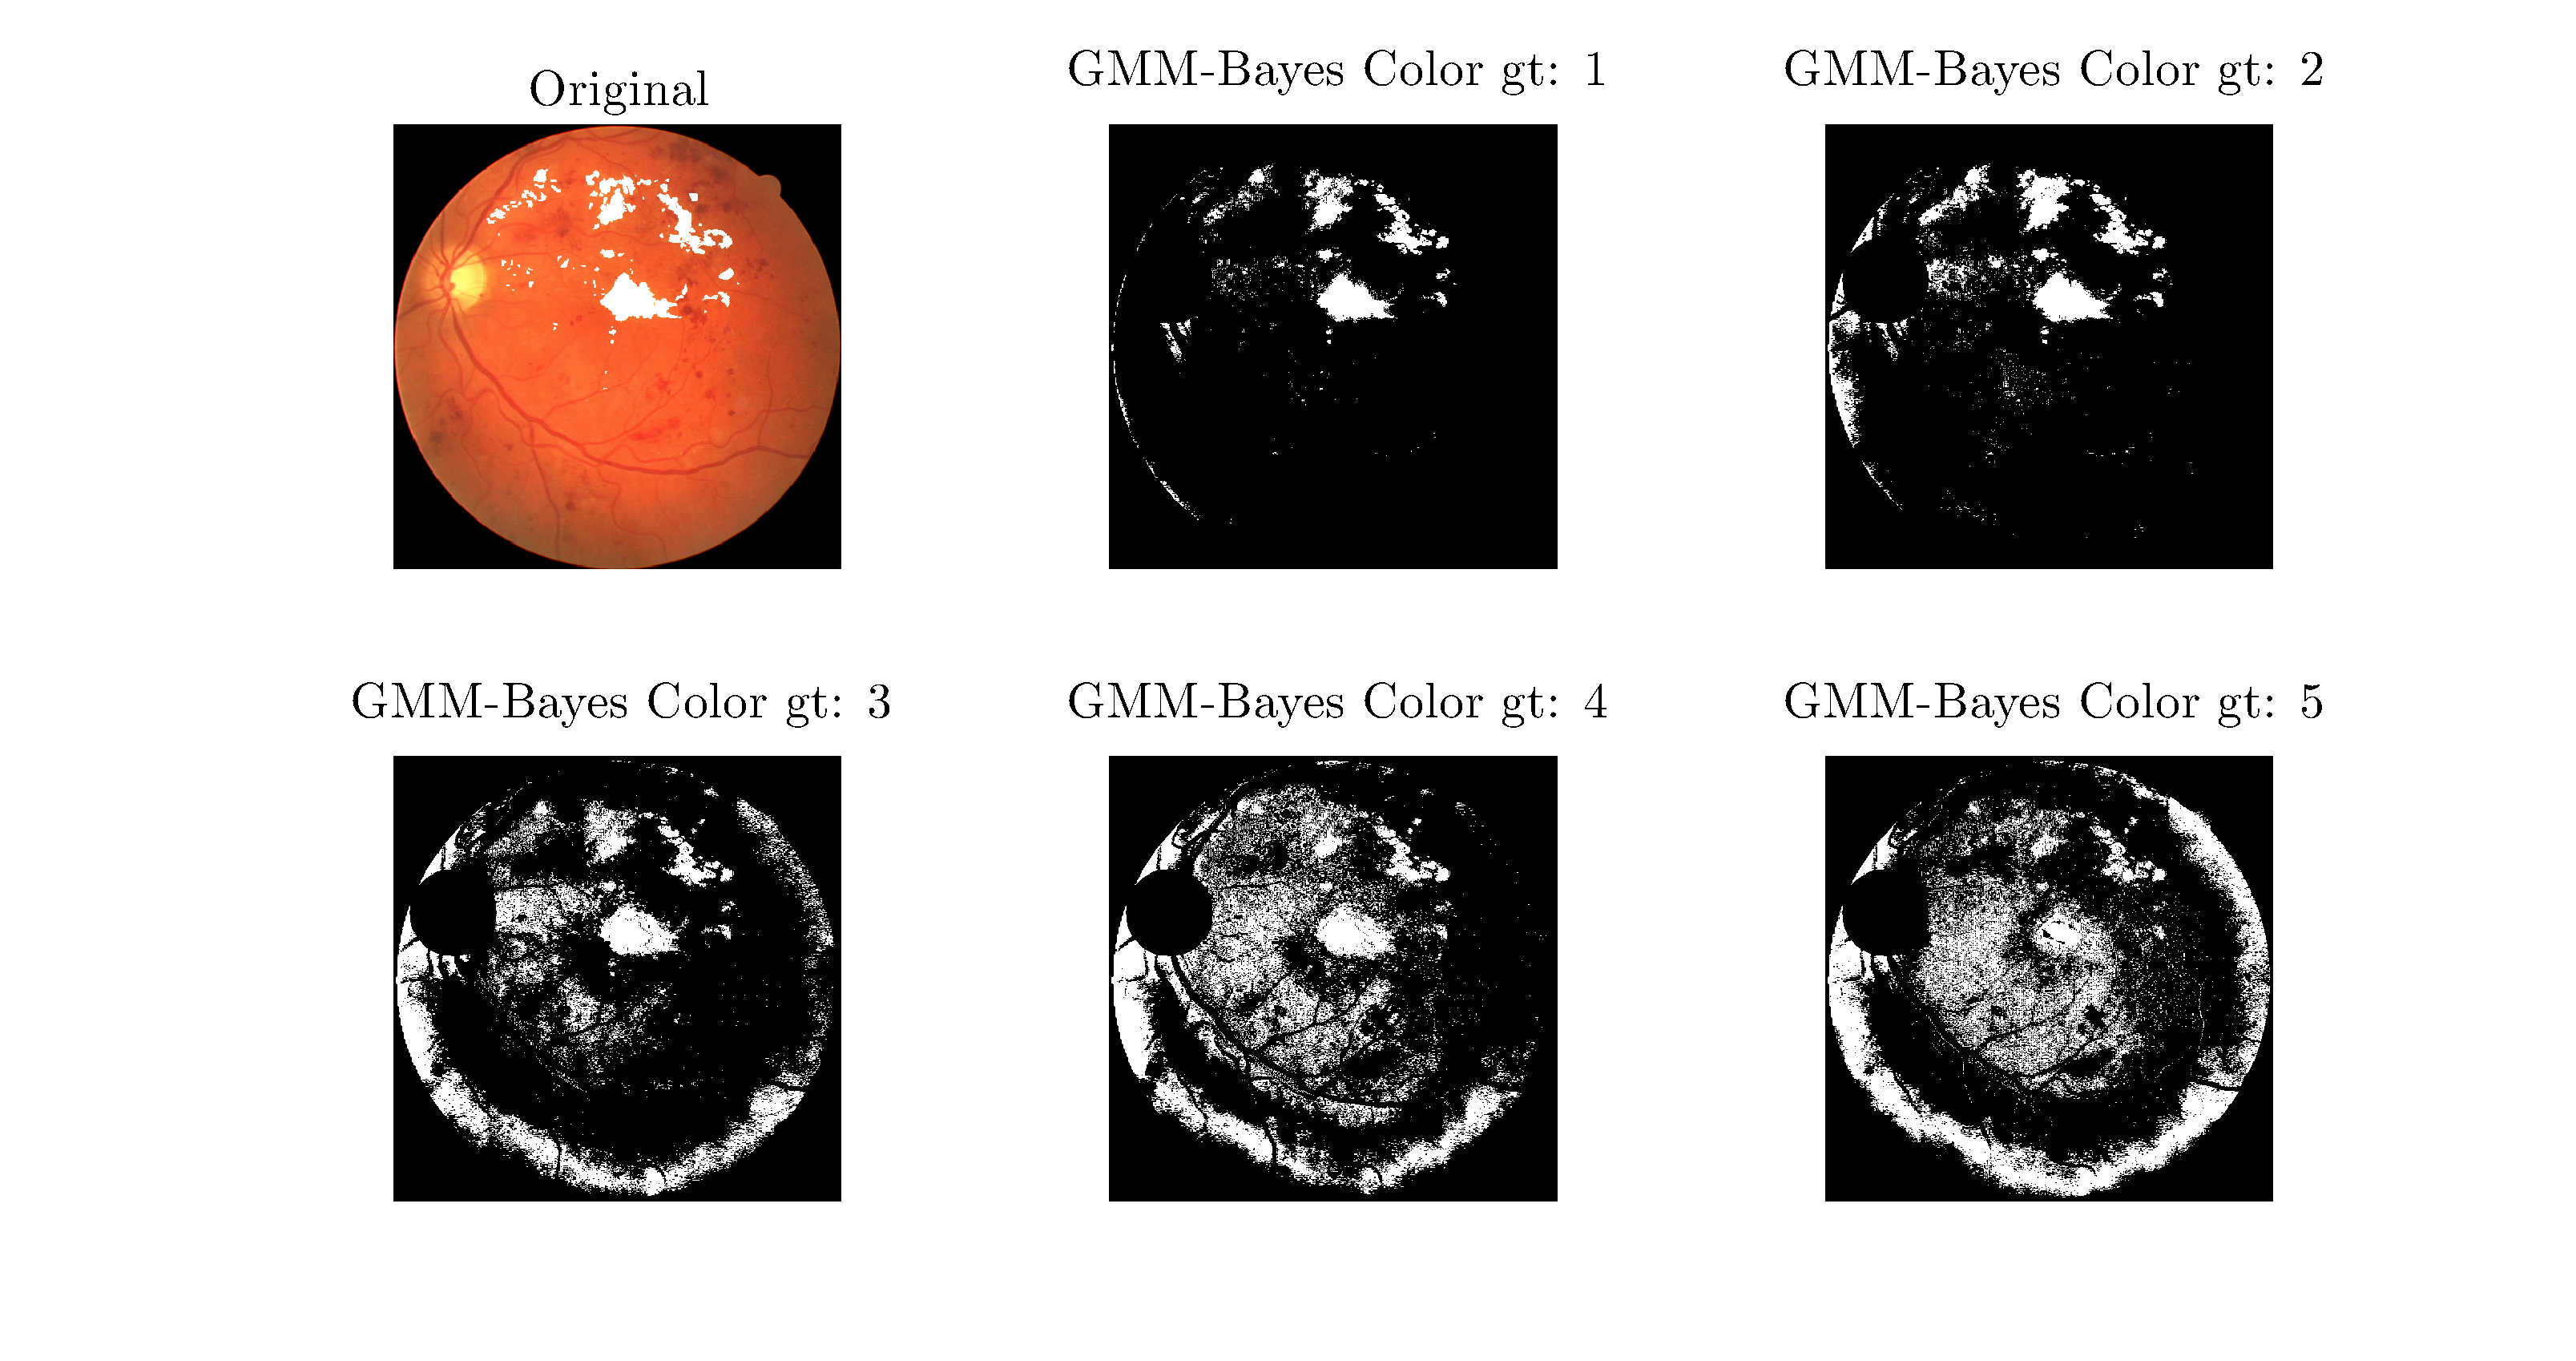
\includegraphics[width=1.4\textwidth,angle=90]{eye_gmmbayes_color_28}     
    \captionof{figure}{Example results of GMM-Bayes classifier using color. The original ground truth is shown superimposed on the image of the eye fundus.
  The segmentation results of the method are shown as a binary image. The results with the accurate ground truth are shown first (1), then the results
  with the three iterations of inaccurate ground truth (2-4), and lastly the results with the most inaccurate ground truth (5).}

\end{minipage}

\begin{minipage}[c]{\textwidth}

    \label{fig:eye28_gmmbayes_edge}
    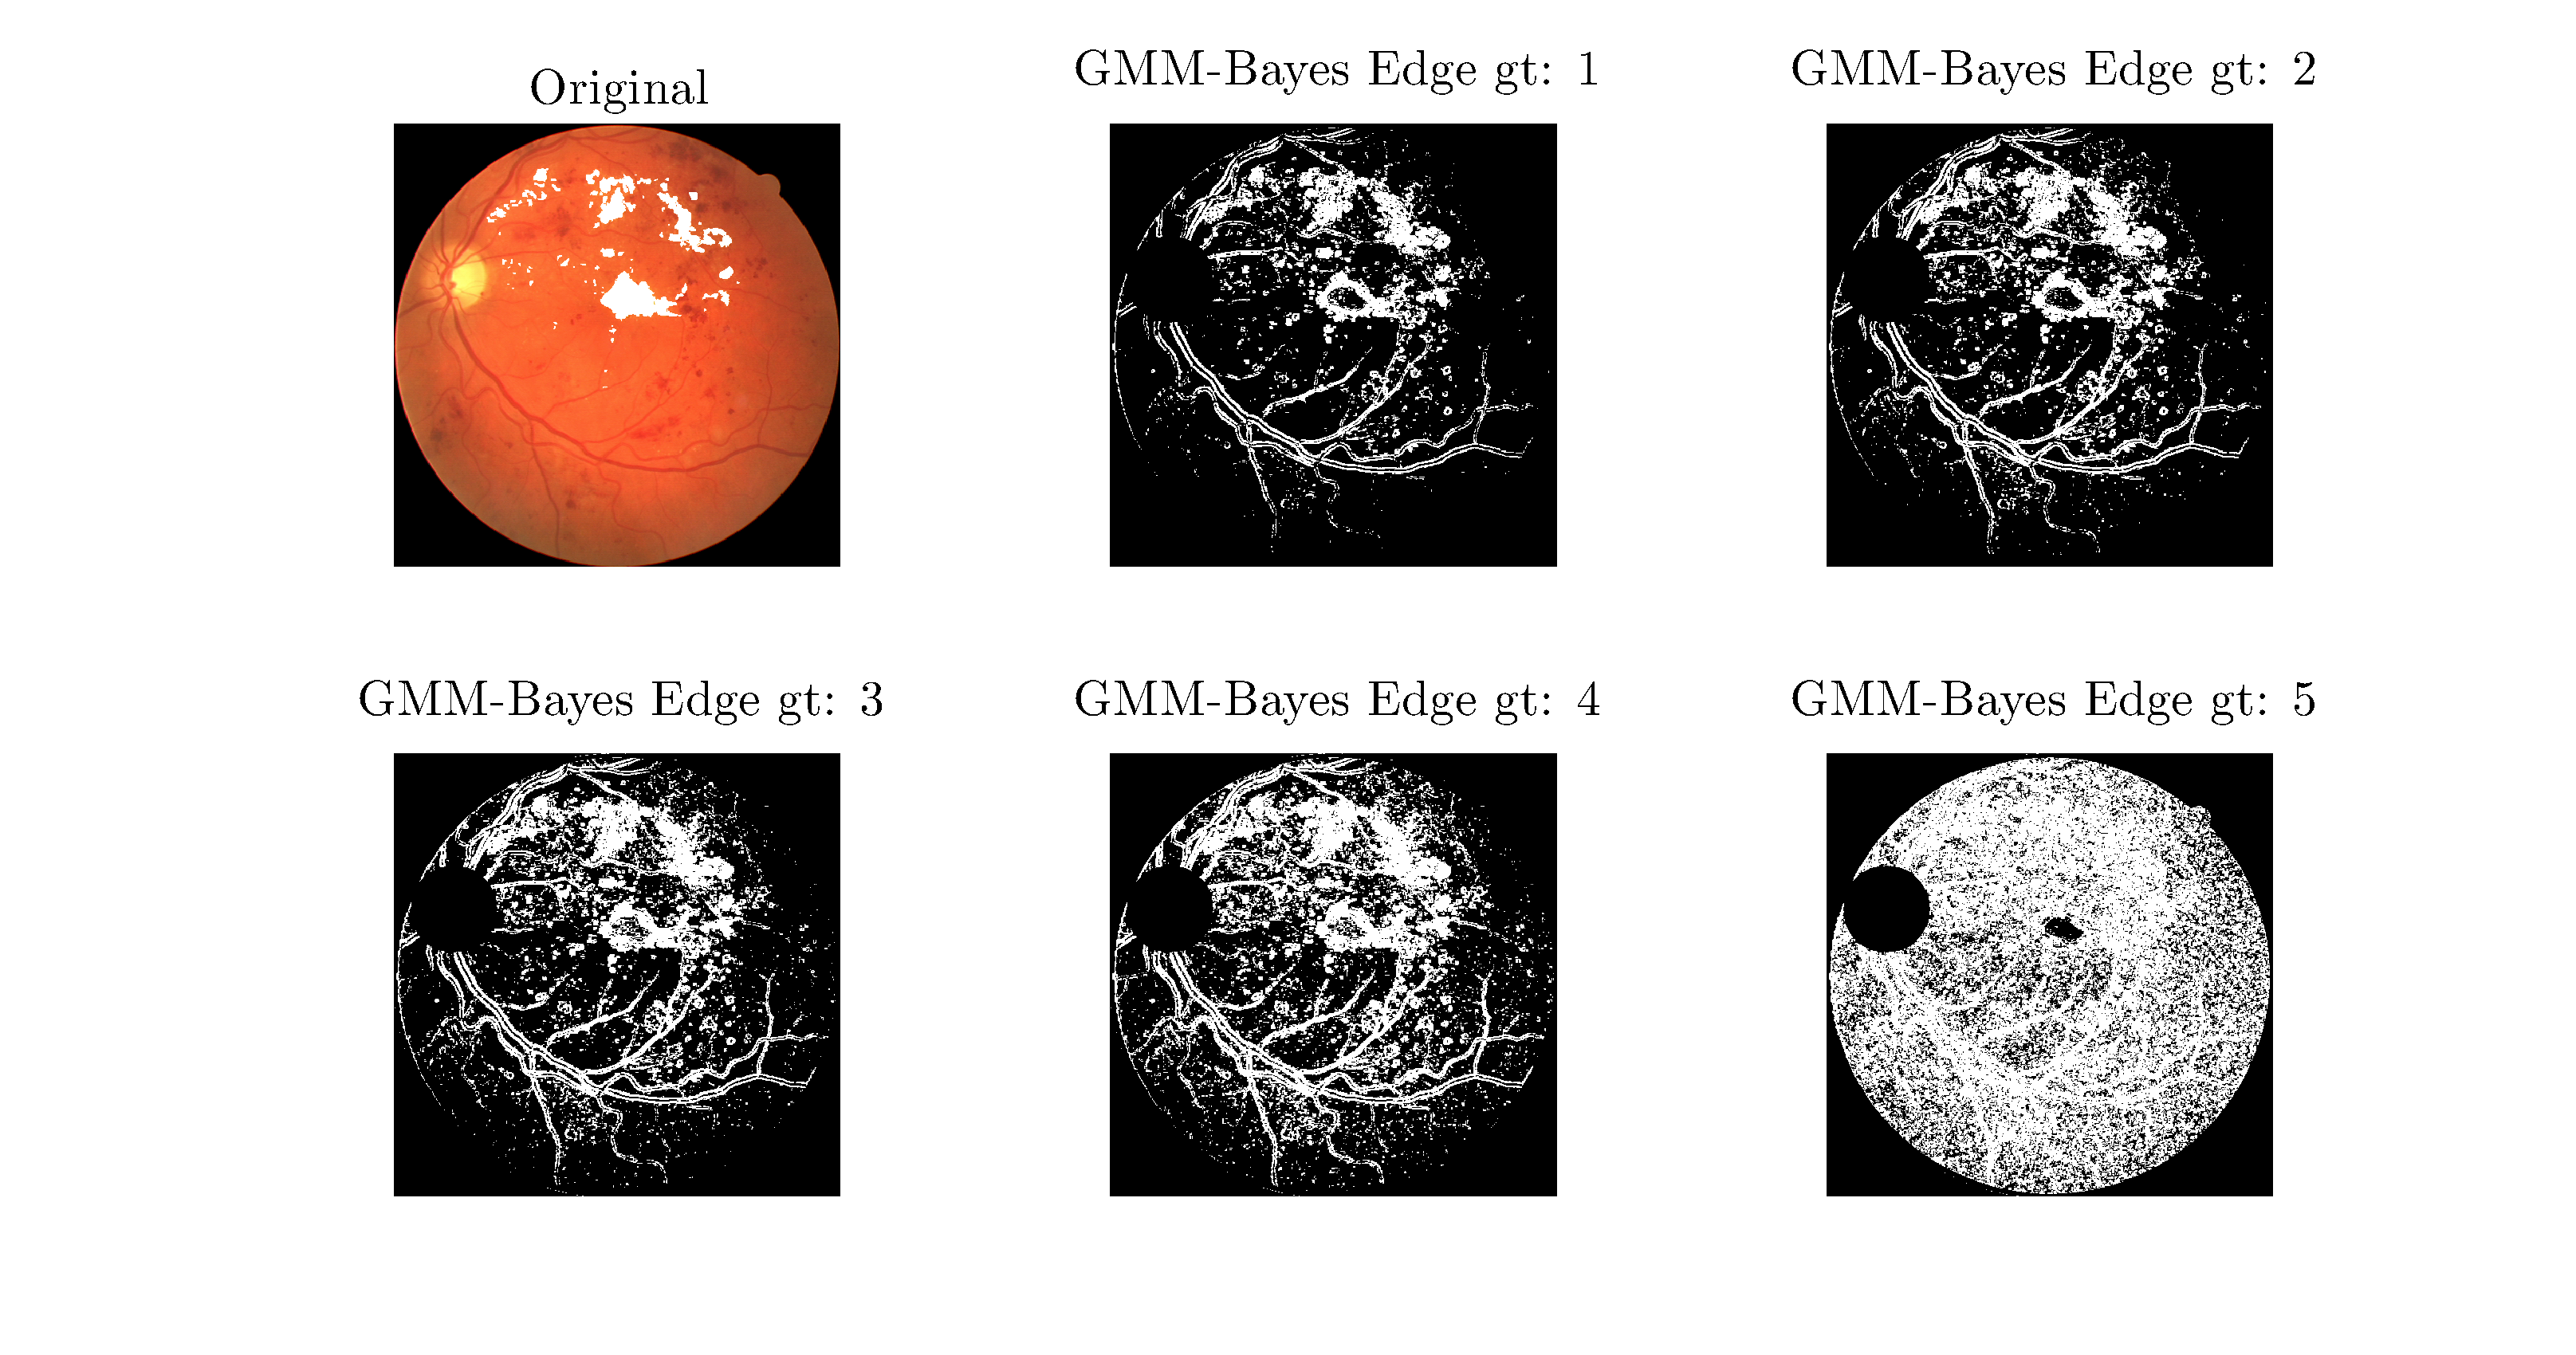
\includegraphics[width=1.4\textwidth,angle=90]{eye_gmmbayes_edge_28}     
    \captionof{figure}{Example results of GMM-Bayes classifier using edge. The original ground truth is shown superimposed on the image of the eye fundus.
  The segmentation results of the method are shown as a binary image. The results with the accurate ground truth are shown first (1), then the results
  with the three iterations of inaccurate ground truth (2-4), and lastly the results with the most inaccurate ground truth (5).}

\end{minipage}

\begin{minipage}[c]{\textwidth}

    \label{fig:eye28_gmmbayes_texture}
    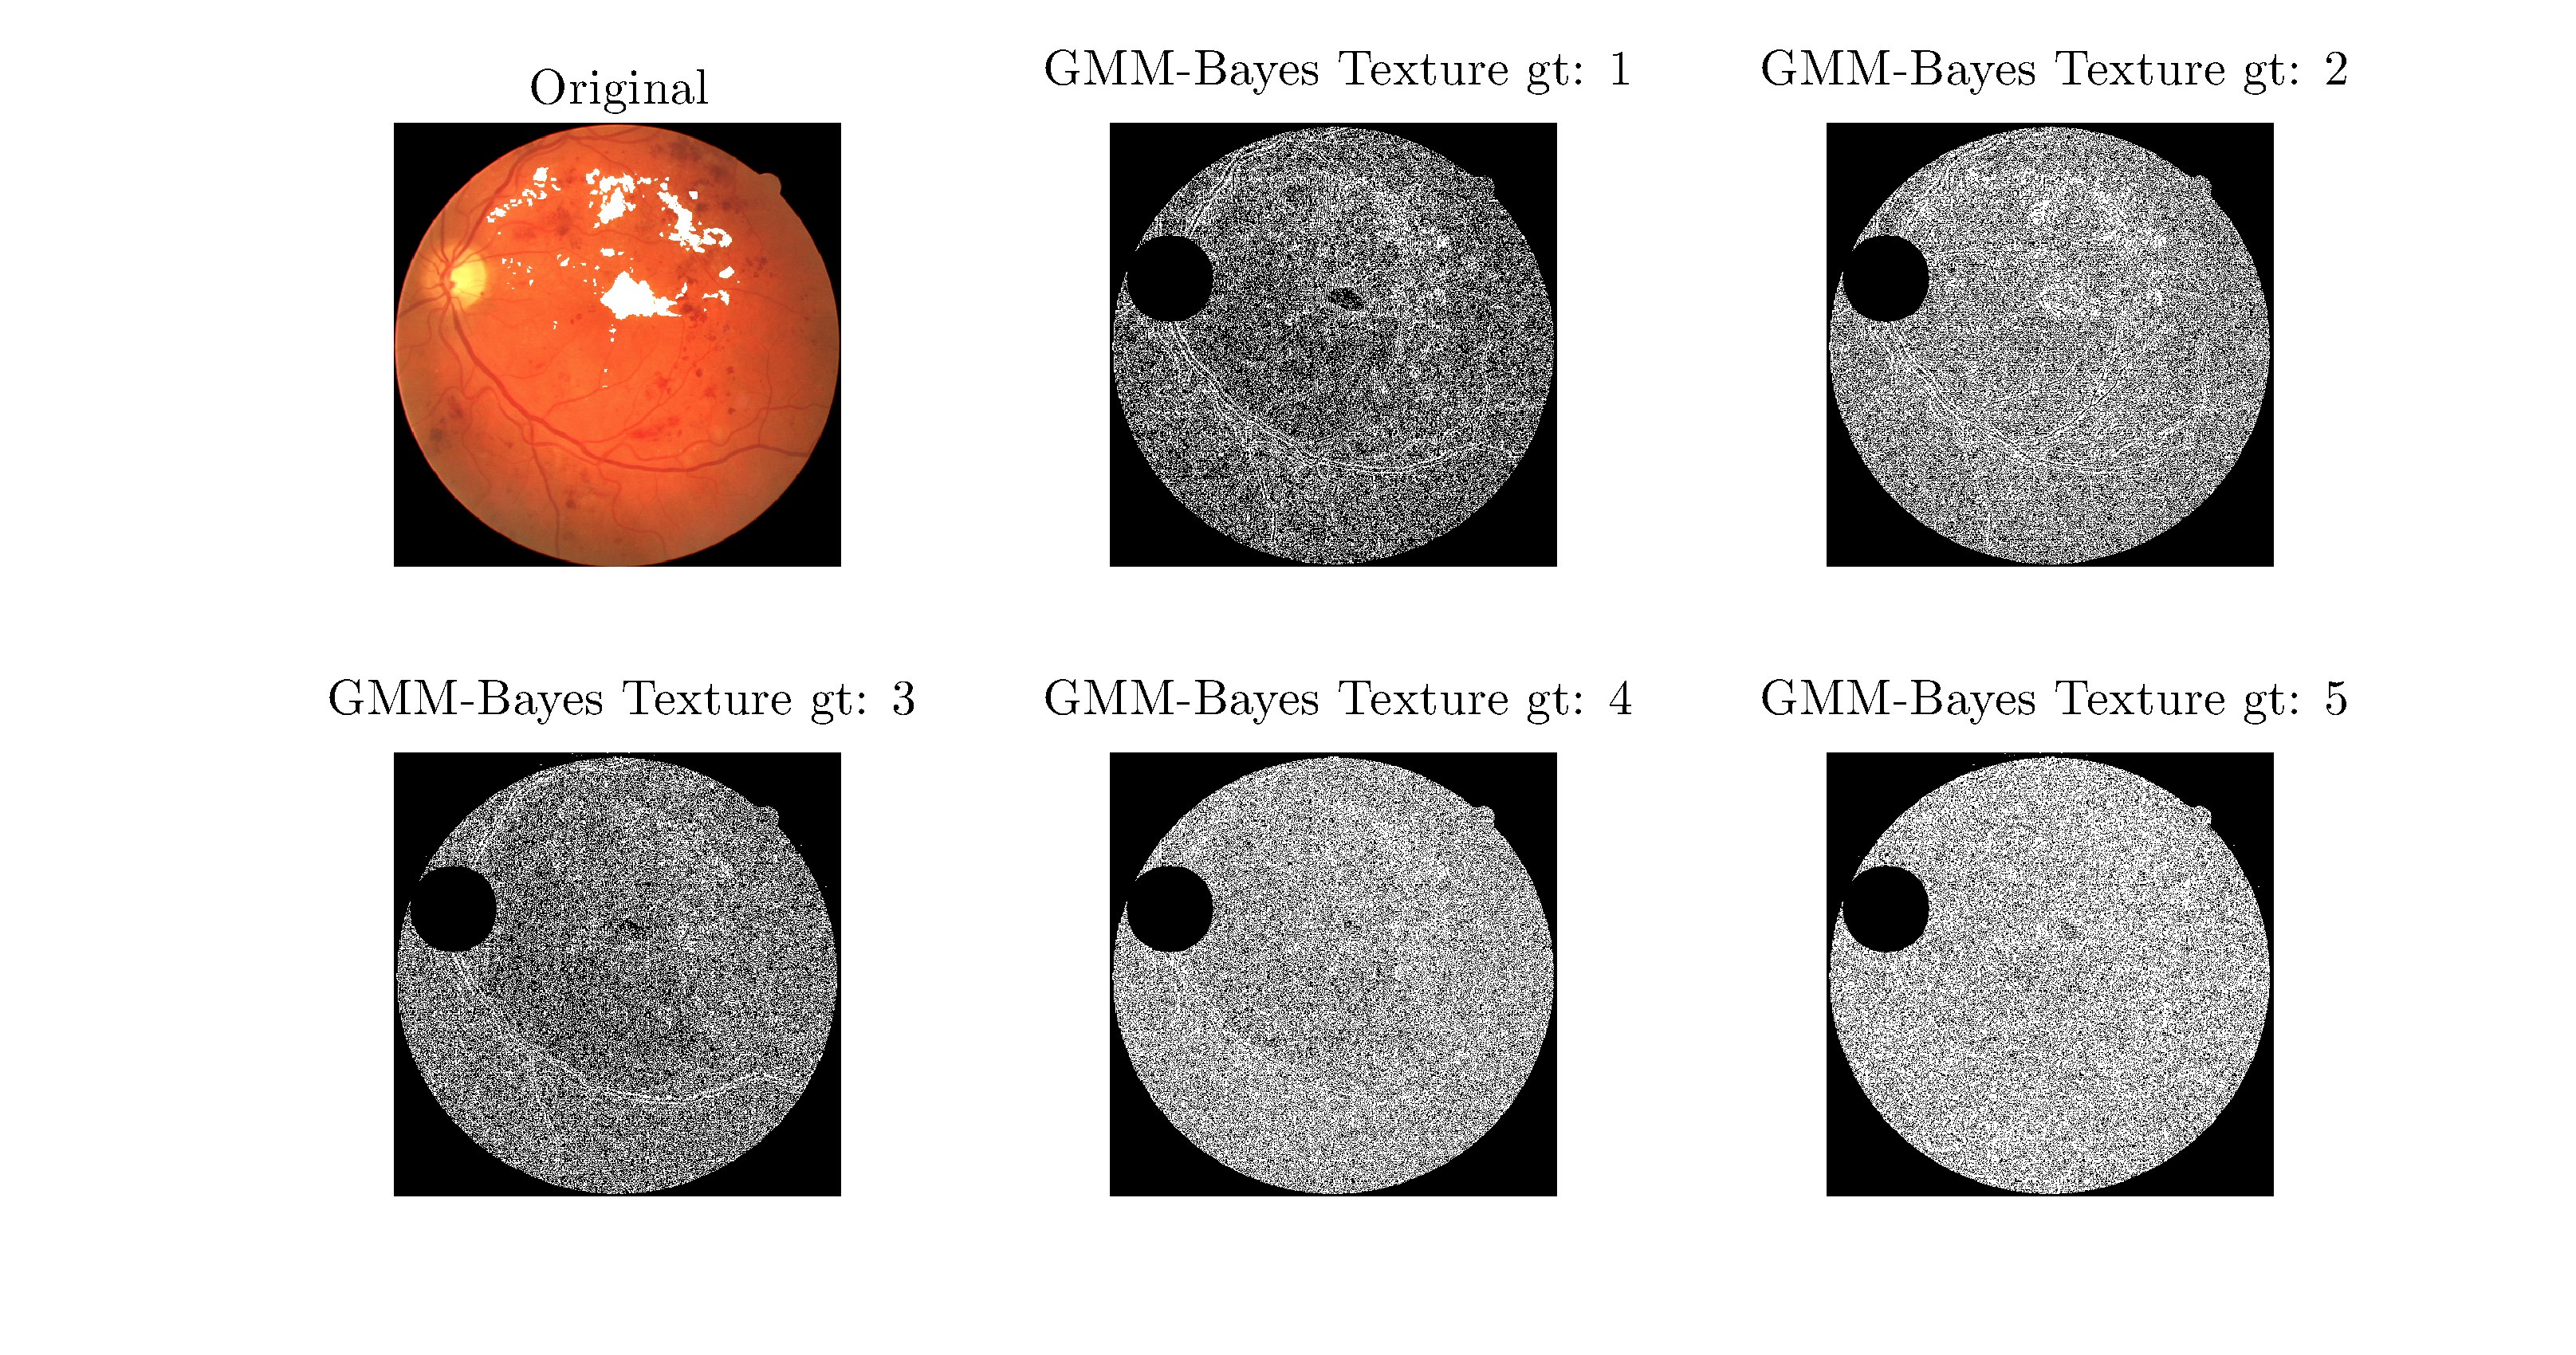
\includegraphics[width=1.4\textwidth,angle=90]{eye_gmmbayes_texture_28}     
    \captionof{figure}{Example results of GMM-Bayes classifier using texture. The original ground truth is shown superimposed on the image of the eye fundus.
  The segmentation results of the method are shown as a binary image. The results with the accurate ground truth are shown first (1), then the results
  with the three iterations of inaccurate ground truth (2-4), and lastly the results with the most inaccurate ground truth (5).}

\end{minipage}

\begin{minipage}[c]{\textwidth}

    \label{fig:eye28_gmmbayes_all}
    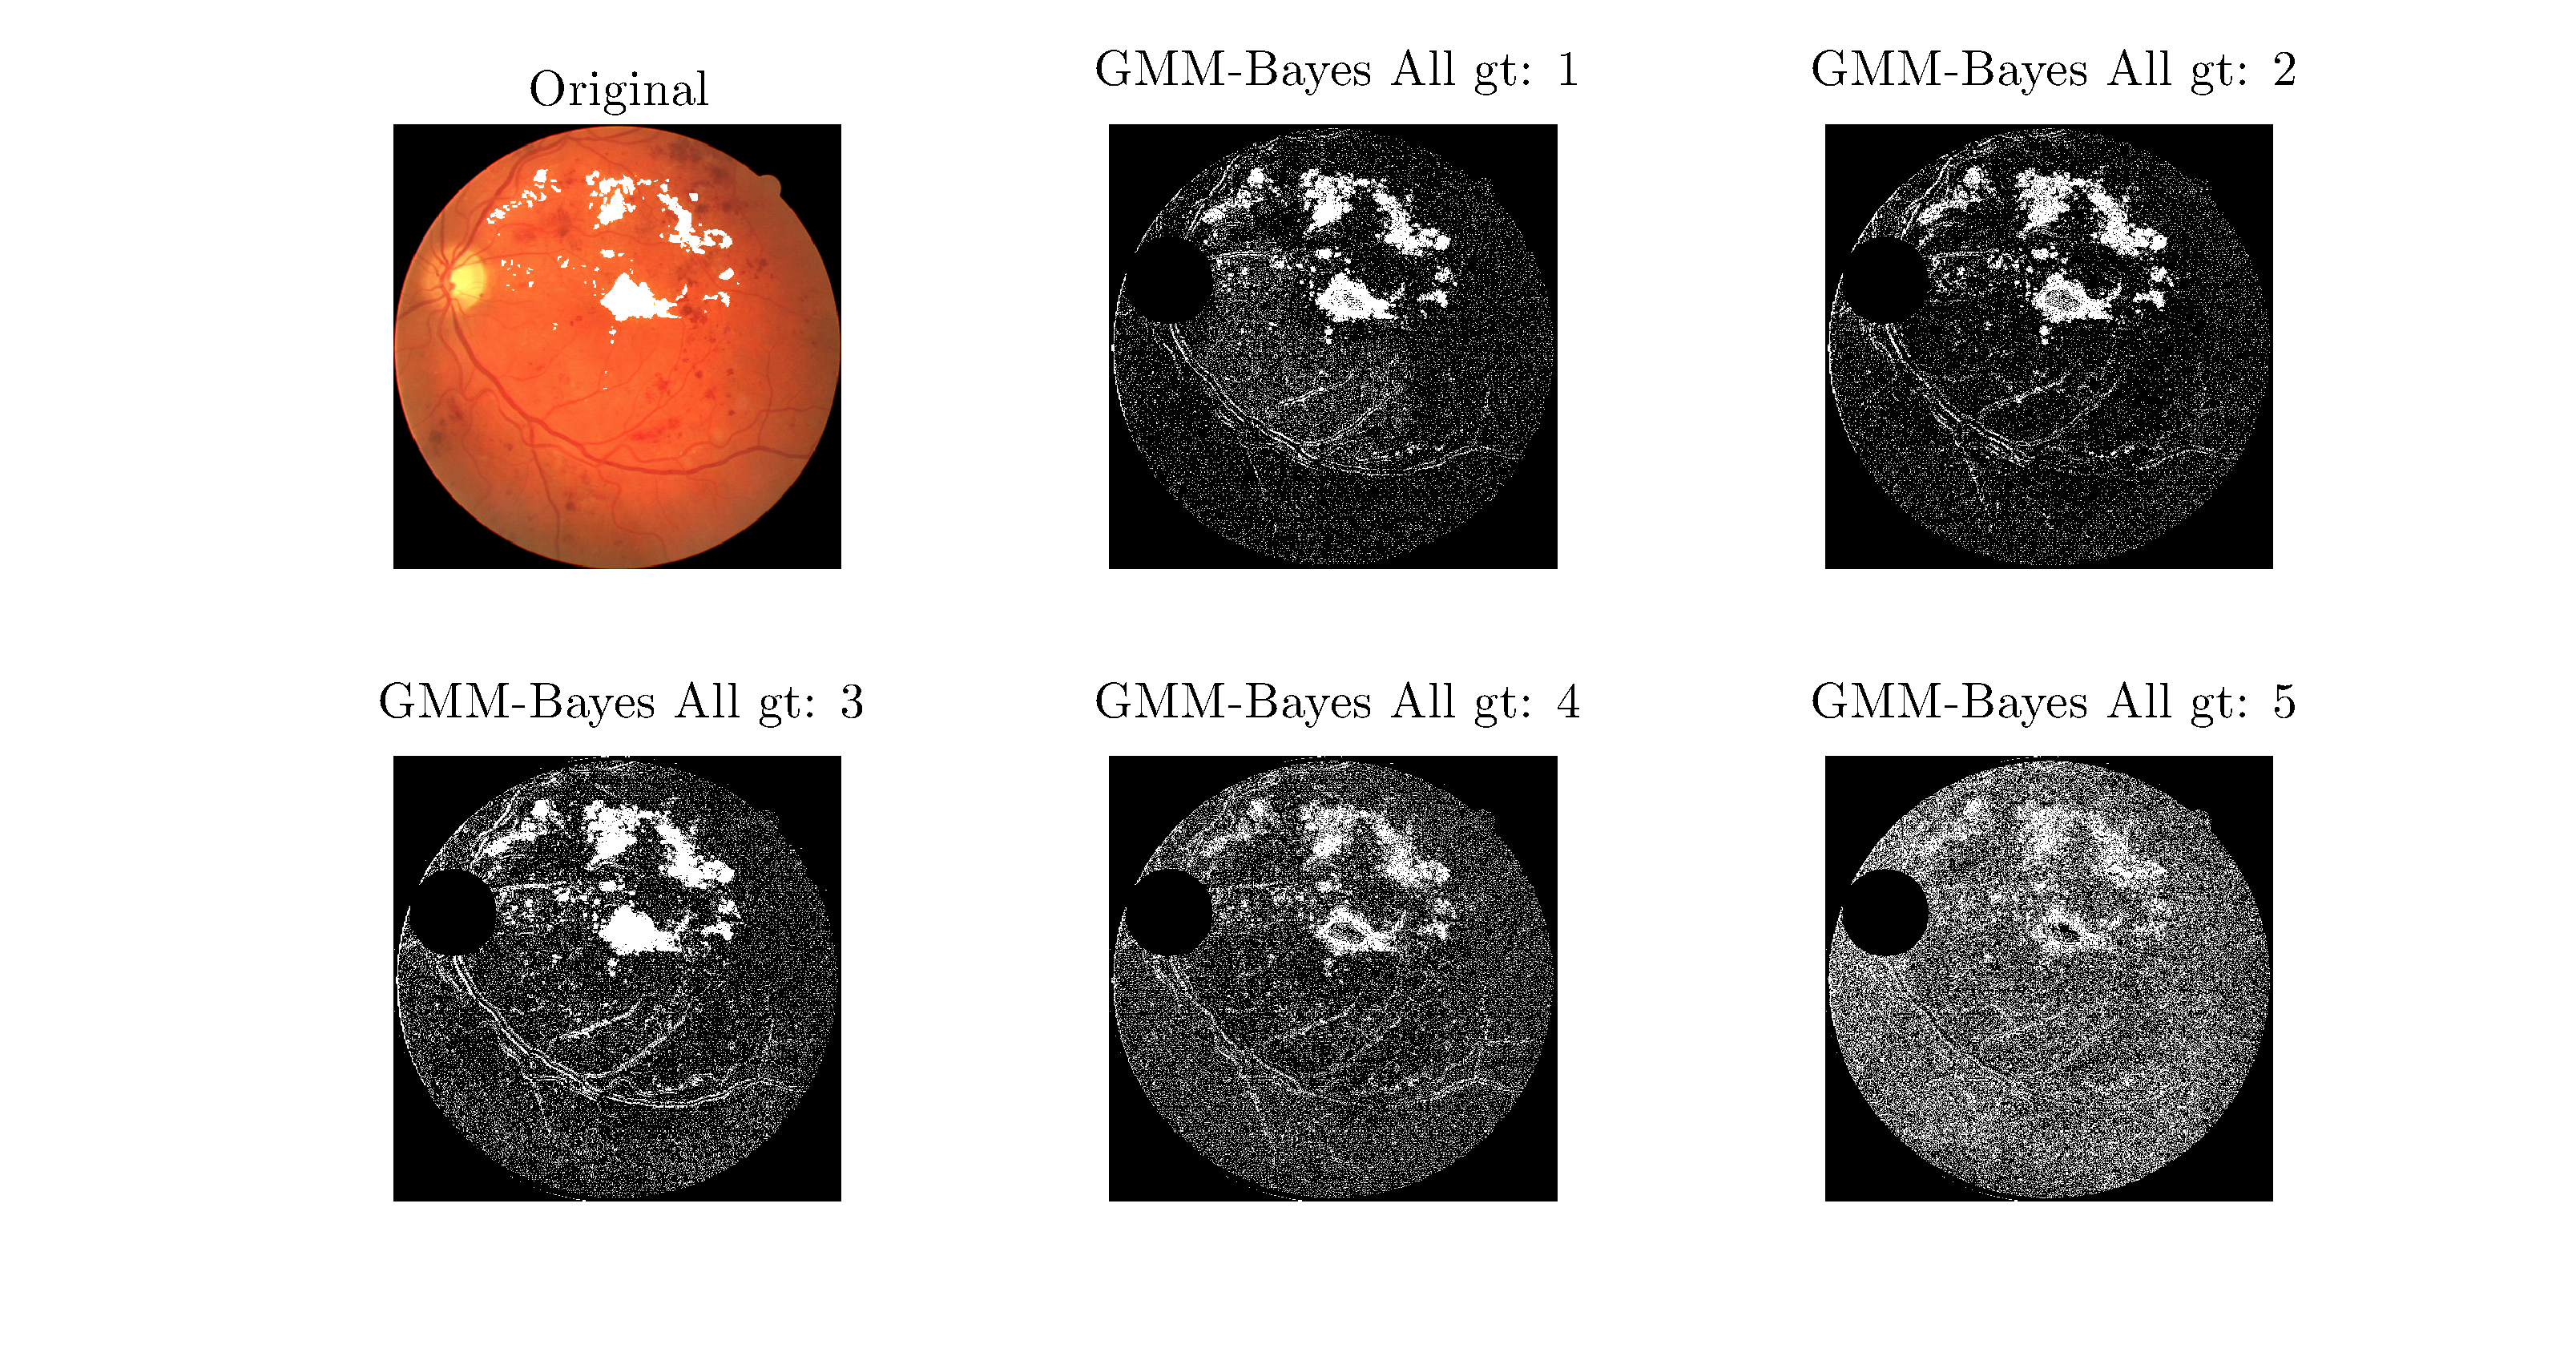
\includegraphics[width=1.4\textwidth,angle=90]{eye_gmmbayes_all_28}     
    \captionof{figure}{Example results of GMM-Bayes classifier using all features. The original ground truth is shown superimposed on the image of the eye fundus.
  The segmentation results of the method are shown as a binary image. The results with the accurate ground truth are shown first (1), then the results
  with the three iterations of inaccurate ground truth (2-4), and lastly the results with the most inaccurate ground truth (5).}

\end{minipage}

\sectionend

\section{Supervised methods' performance using gray world pictures}
\label{app:grayworld}

\begin{minipage}{\linewidth}
    \centering
    \begin{figure}[H]
	\subfloat[]{
	    \label{fig:grayworld_bayes_sens}
	    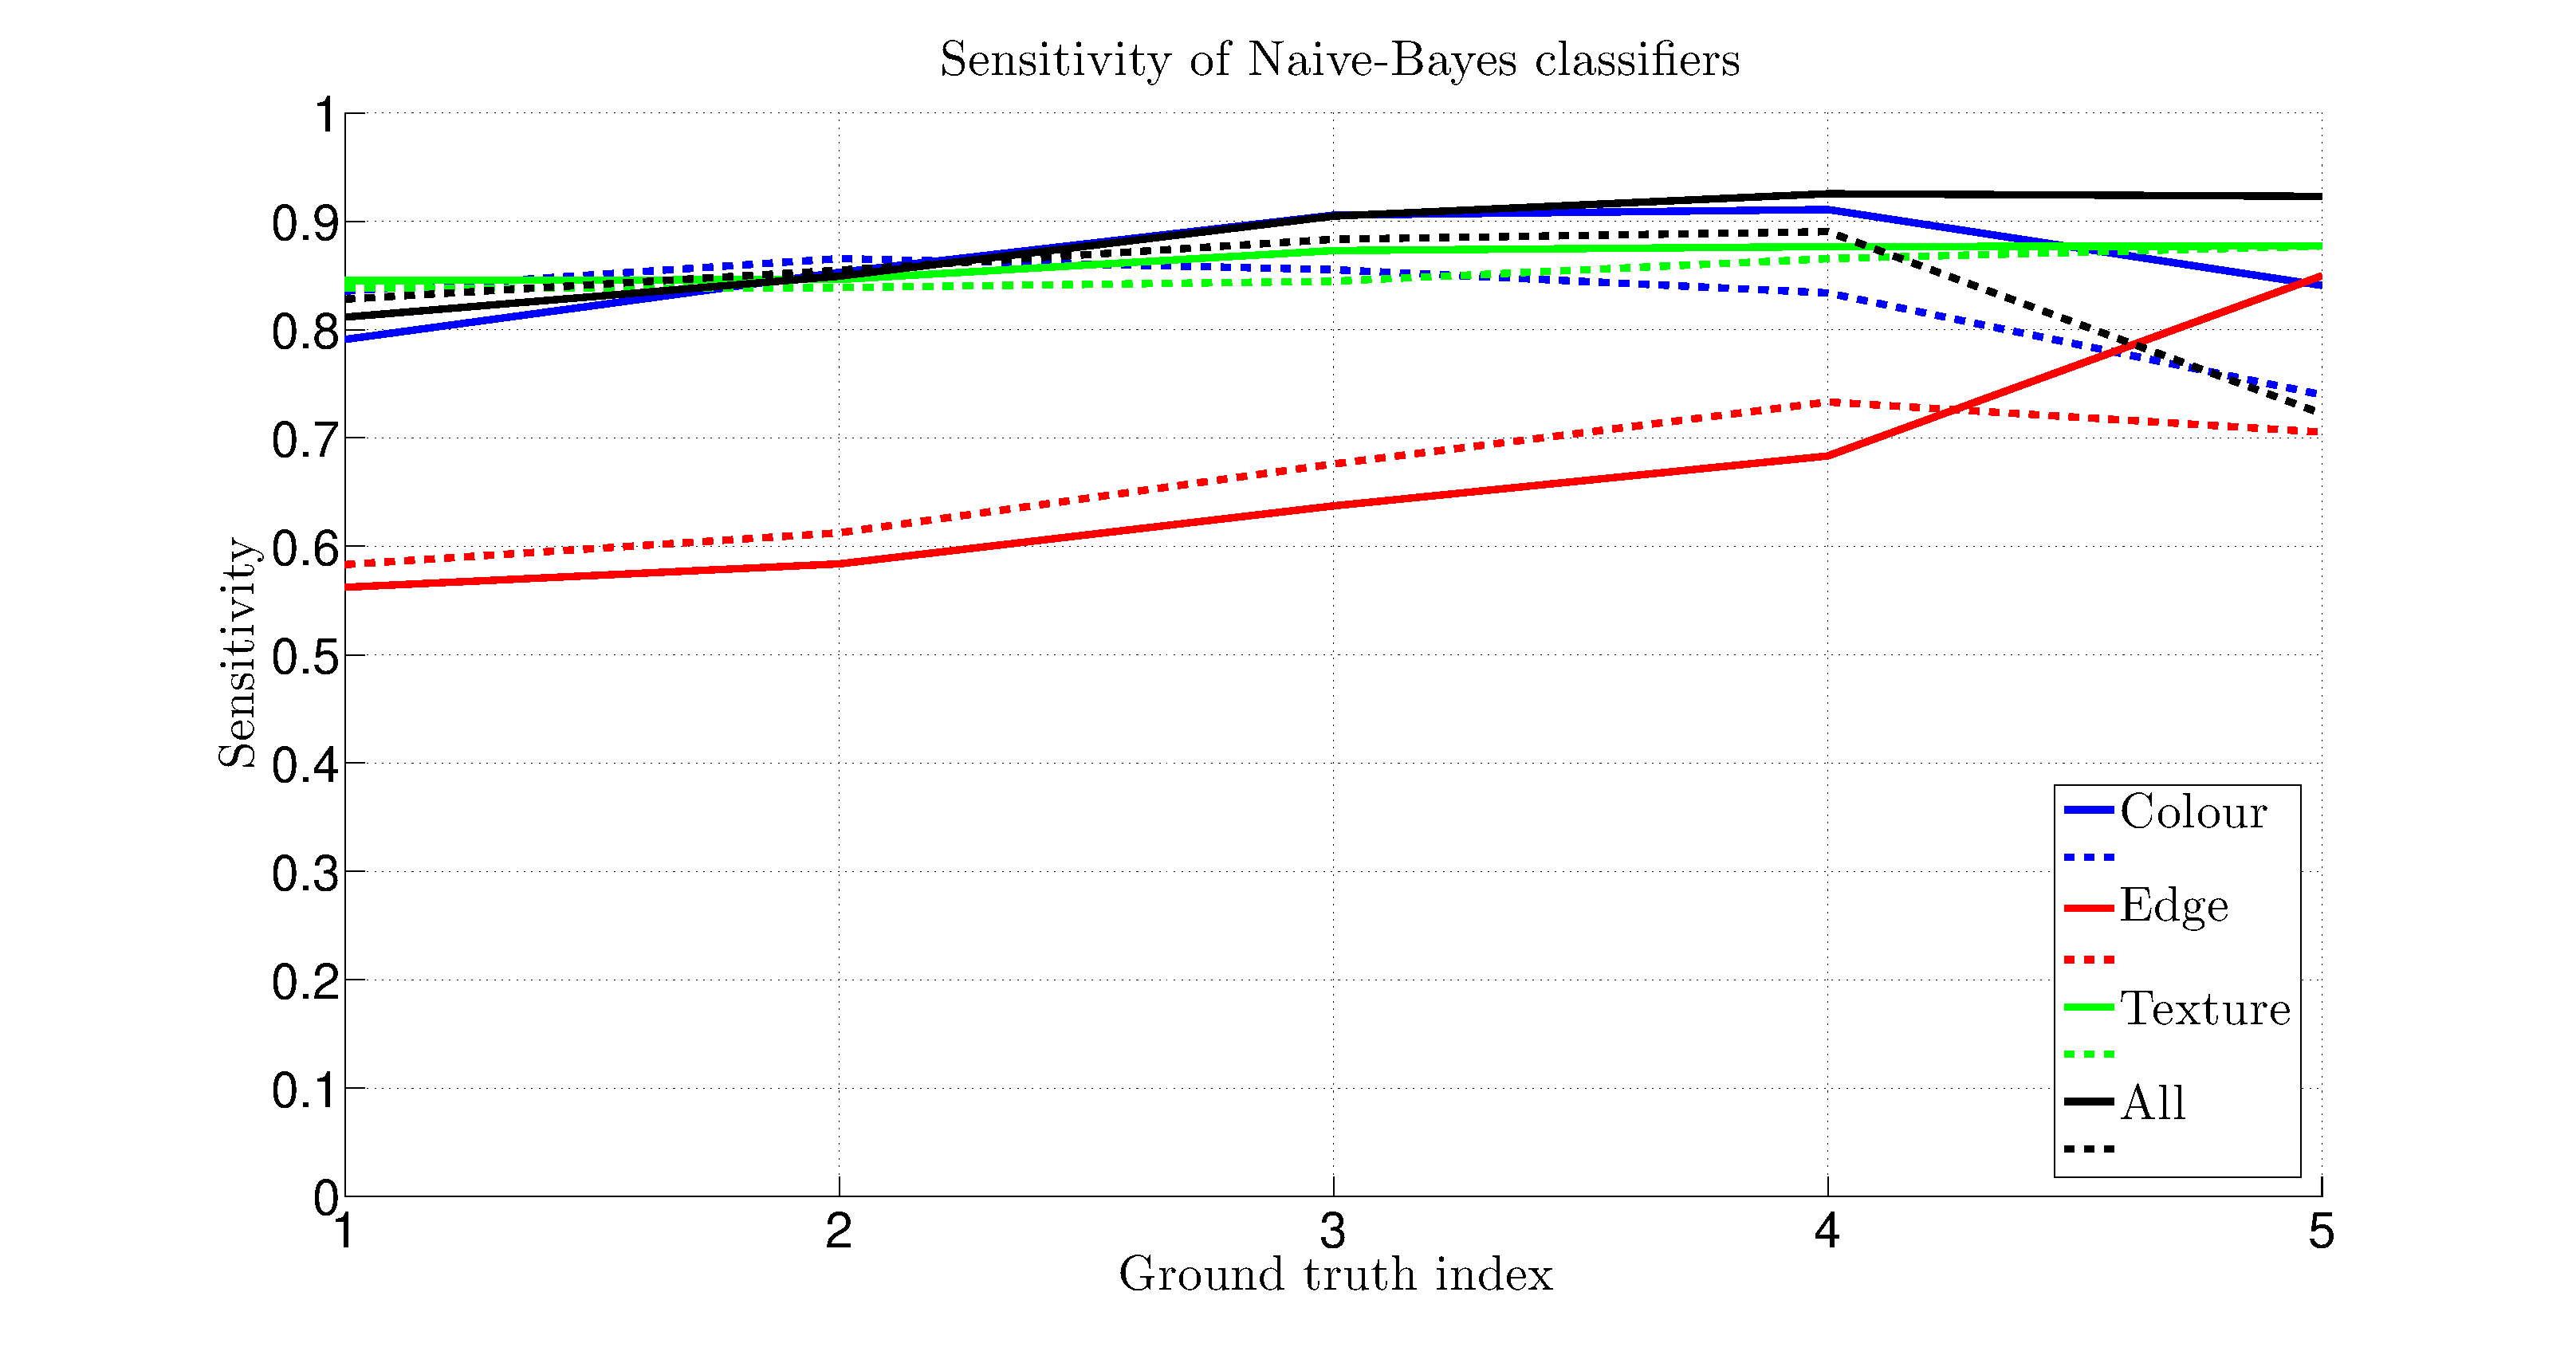
\includegraphics[width=0.95\textwidth]{hist_bayes_sens_imgset2}
	}
	
	\subfloat[]{
	    \label{fig:grayworld_bayes_spec}
	    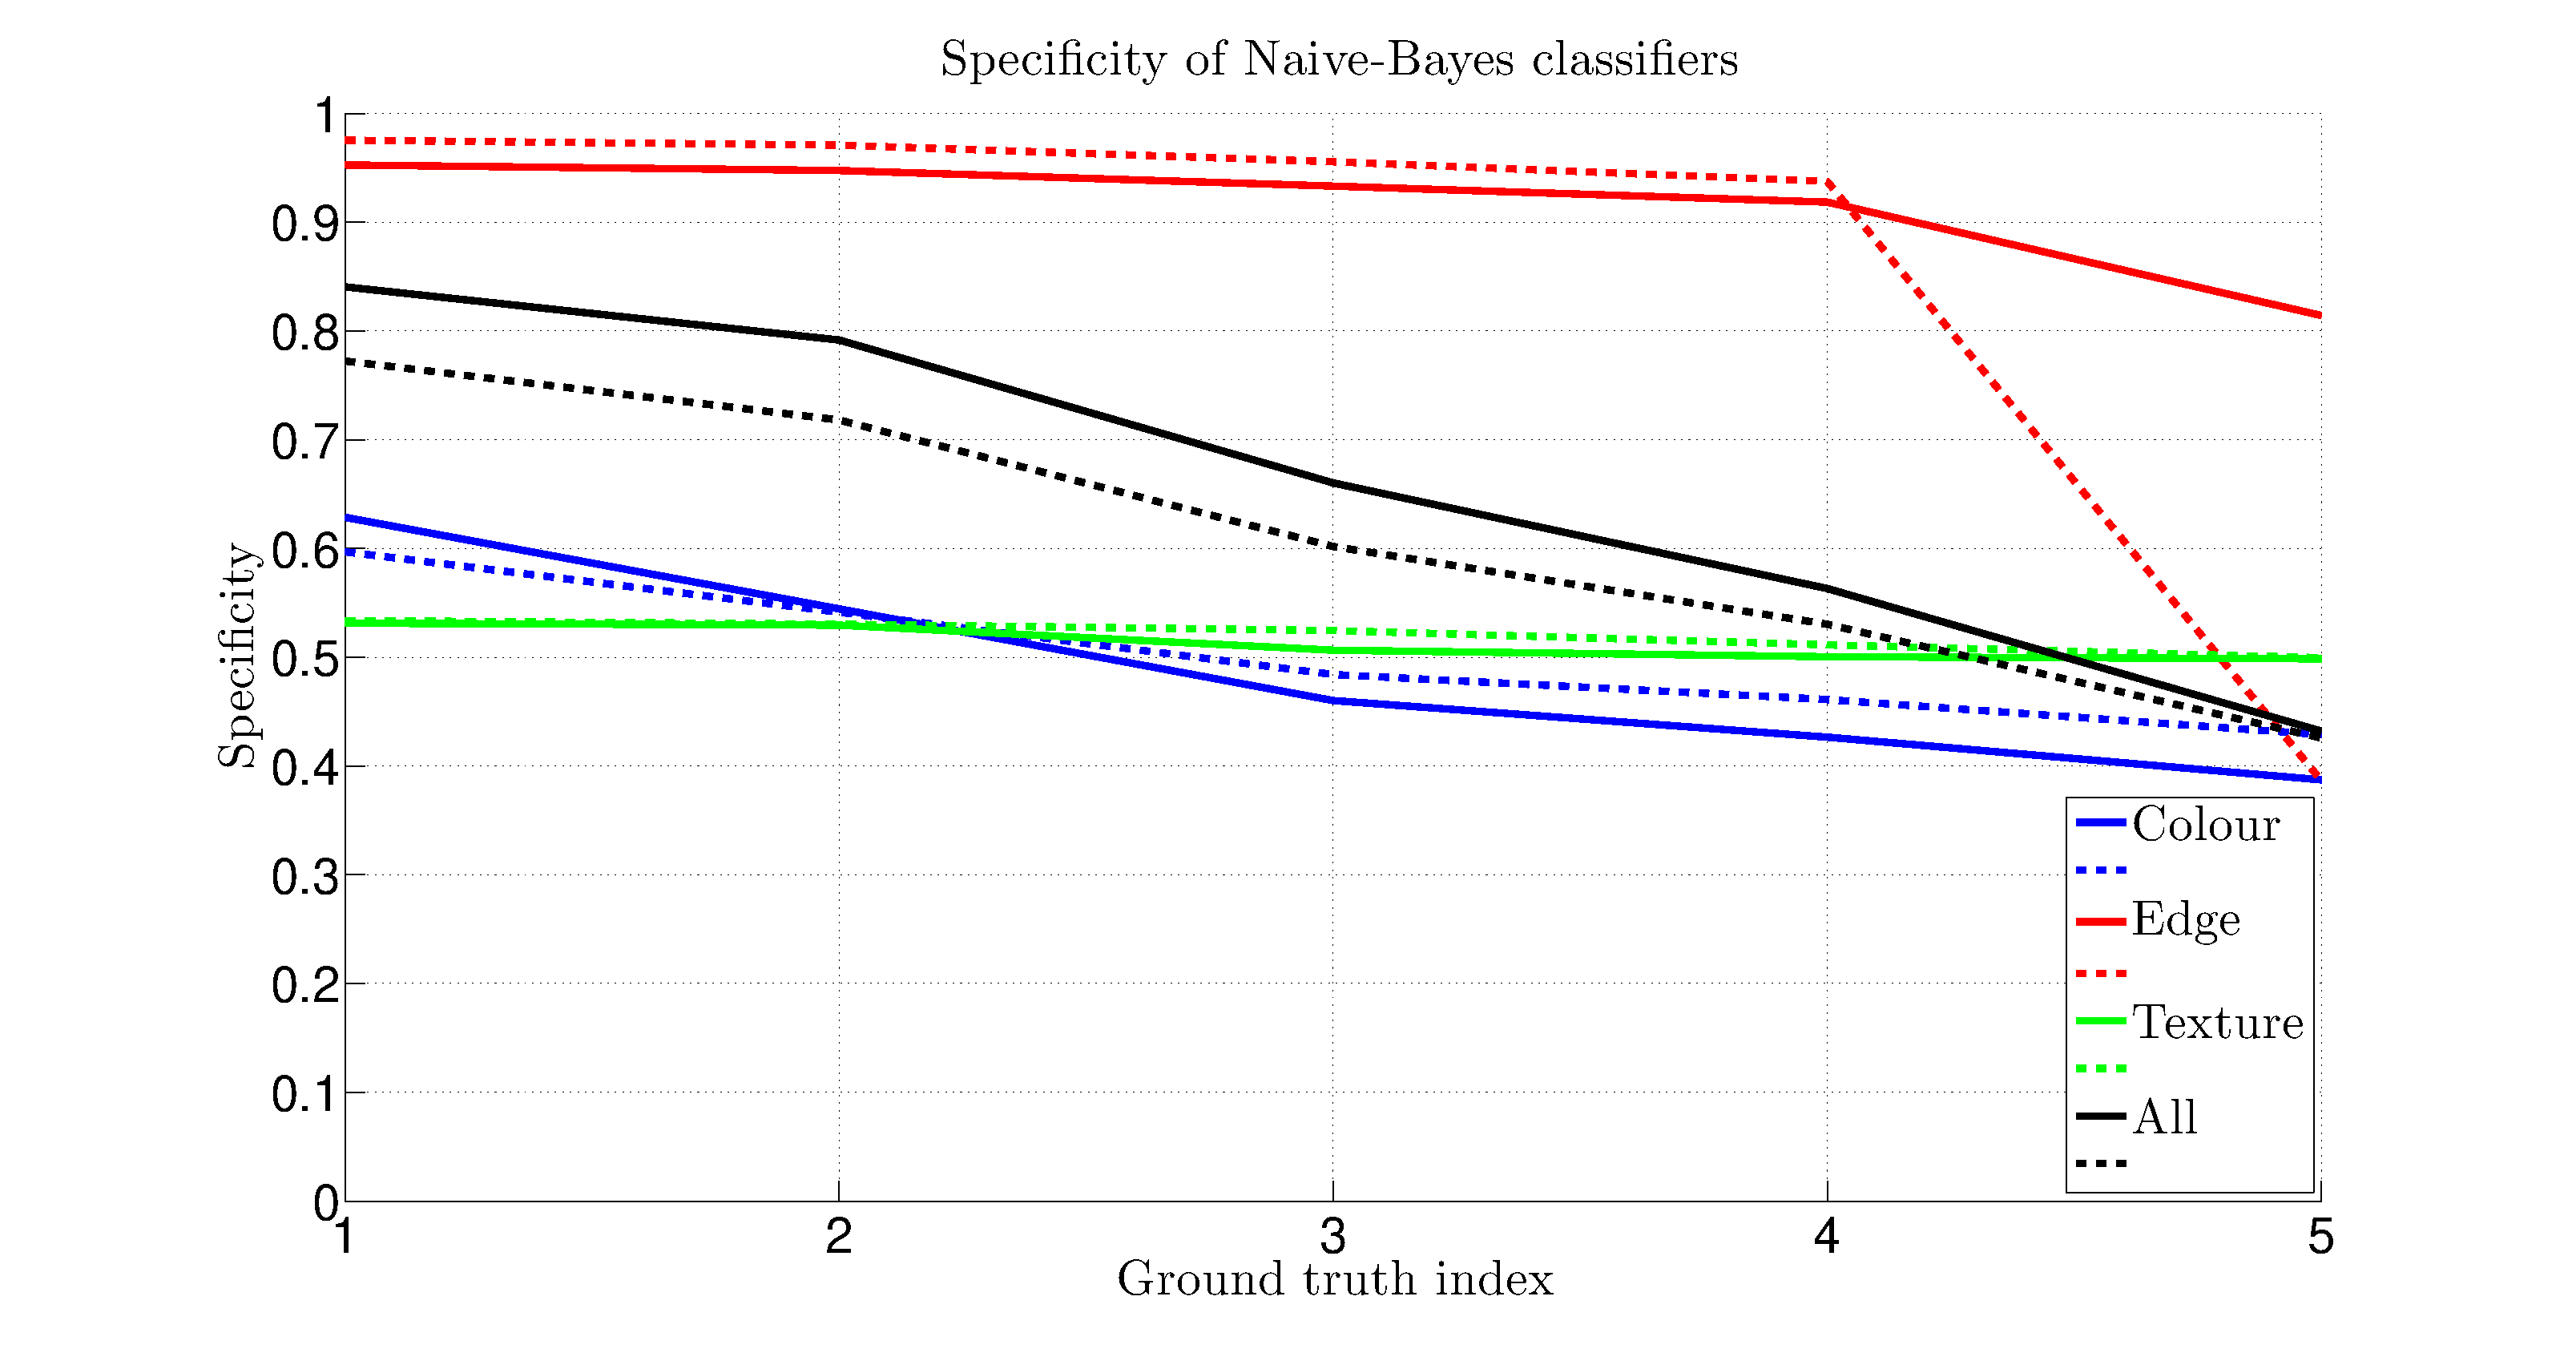
\includegraphics[width=0.95\textwidth]{hist_bayes_spec_imgset2}
	}
	
	\caption[moving]{Performance of Na�ve-Bayes classifiers using gray world images:
	\subref{fig:grayworld_bayes_sens} sensitivity,
	\subref{fig:grayworld_bayes_spec} specificity. }
	\label{fig:grayworld_bayes}
    \end{figure}
\end{minipage}

\begin{minipage}{\linewidth}
    \centering
    \begin{figure}[H]
	\subfloat[]{
	    \label{fig:grayworld_gmmbayes_sens}
	    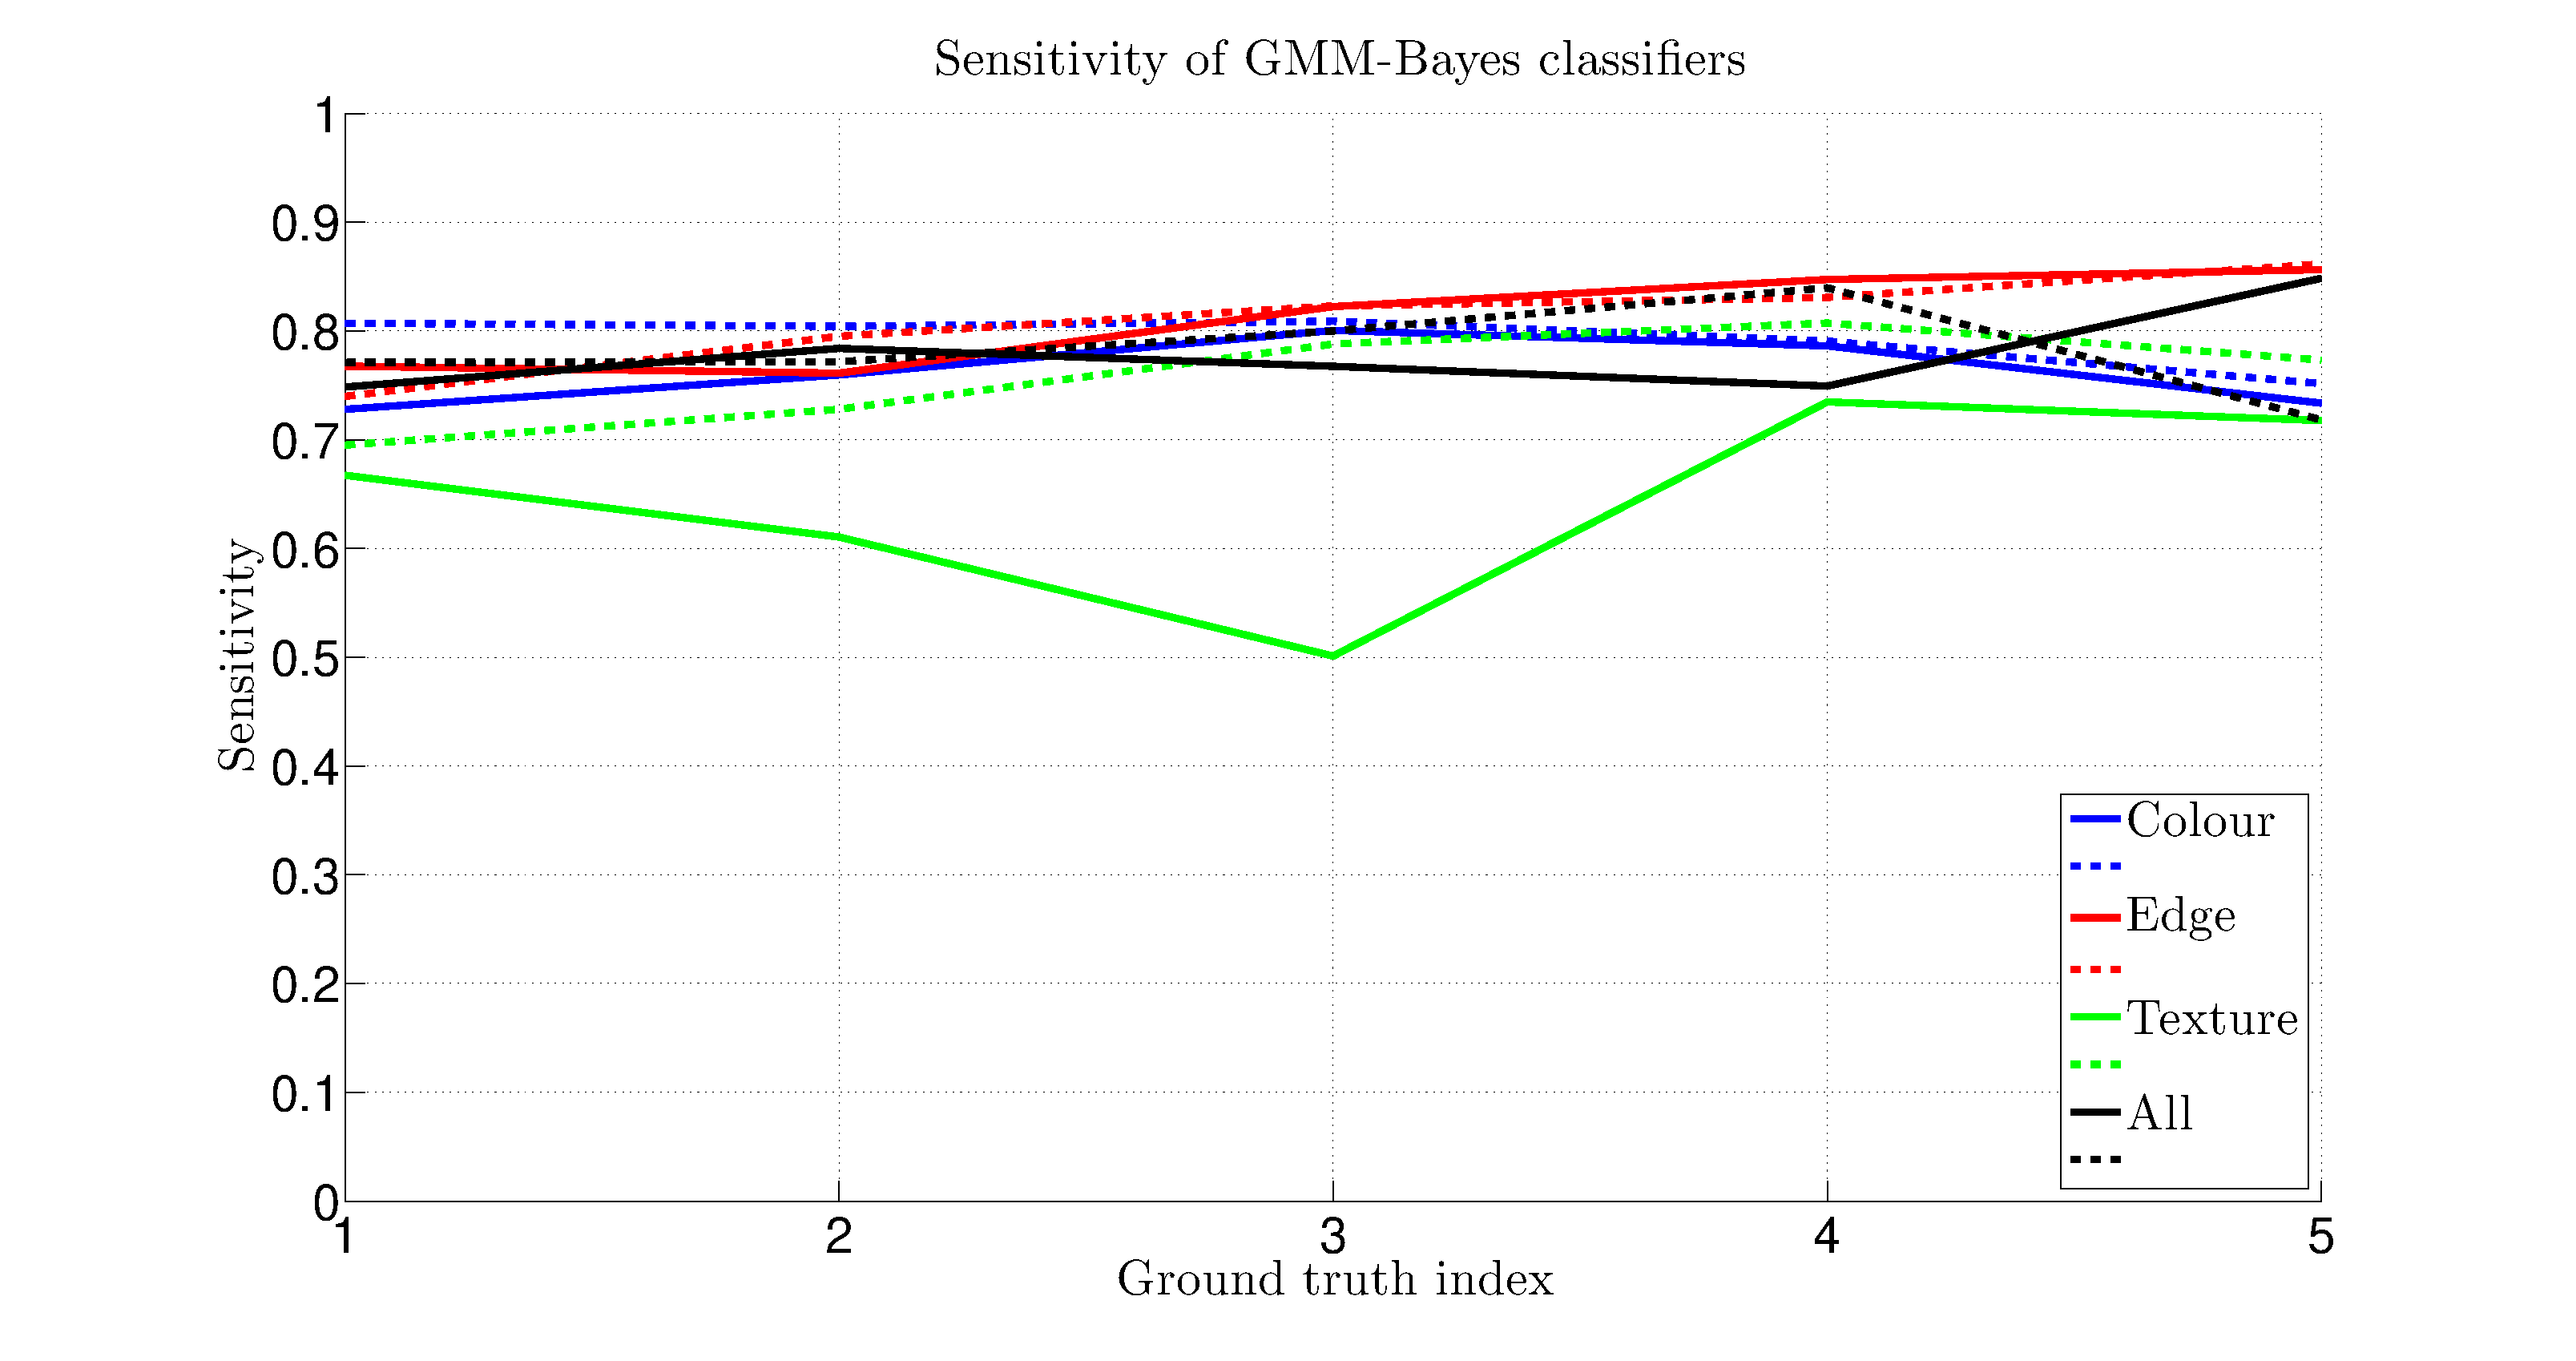
\includegraphics[width=0.95\textwidth]{hist_gmmbayes_sens_imgset2}
	}

	\subfloat[]{
	    \label{fig:grayworld_gmmbayes_spec}
	    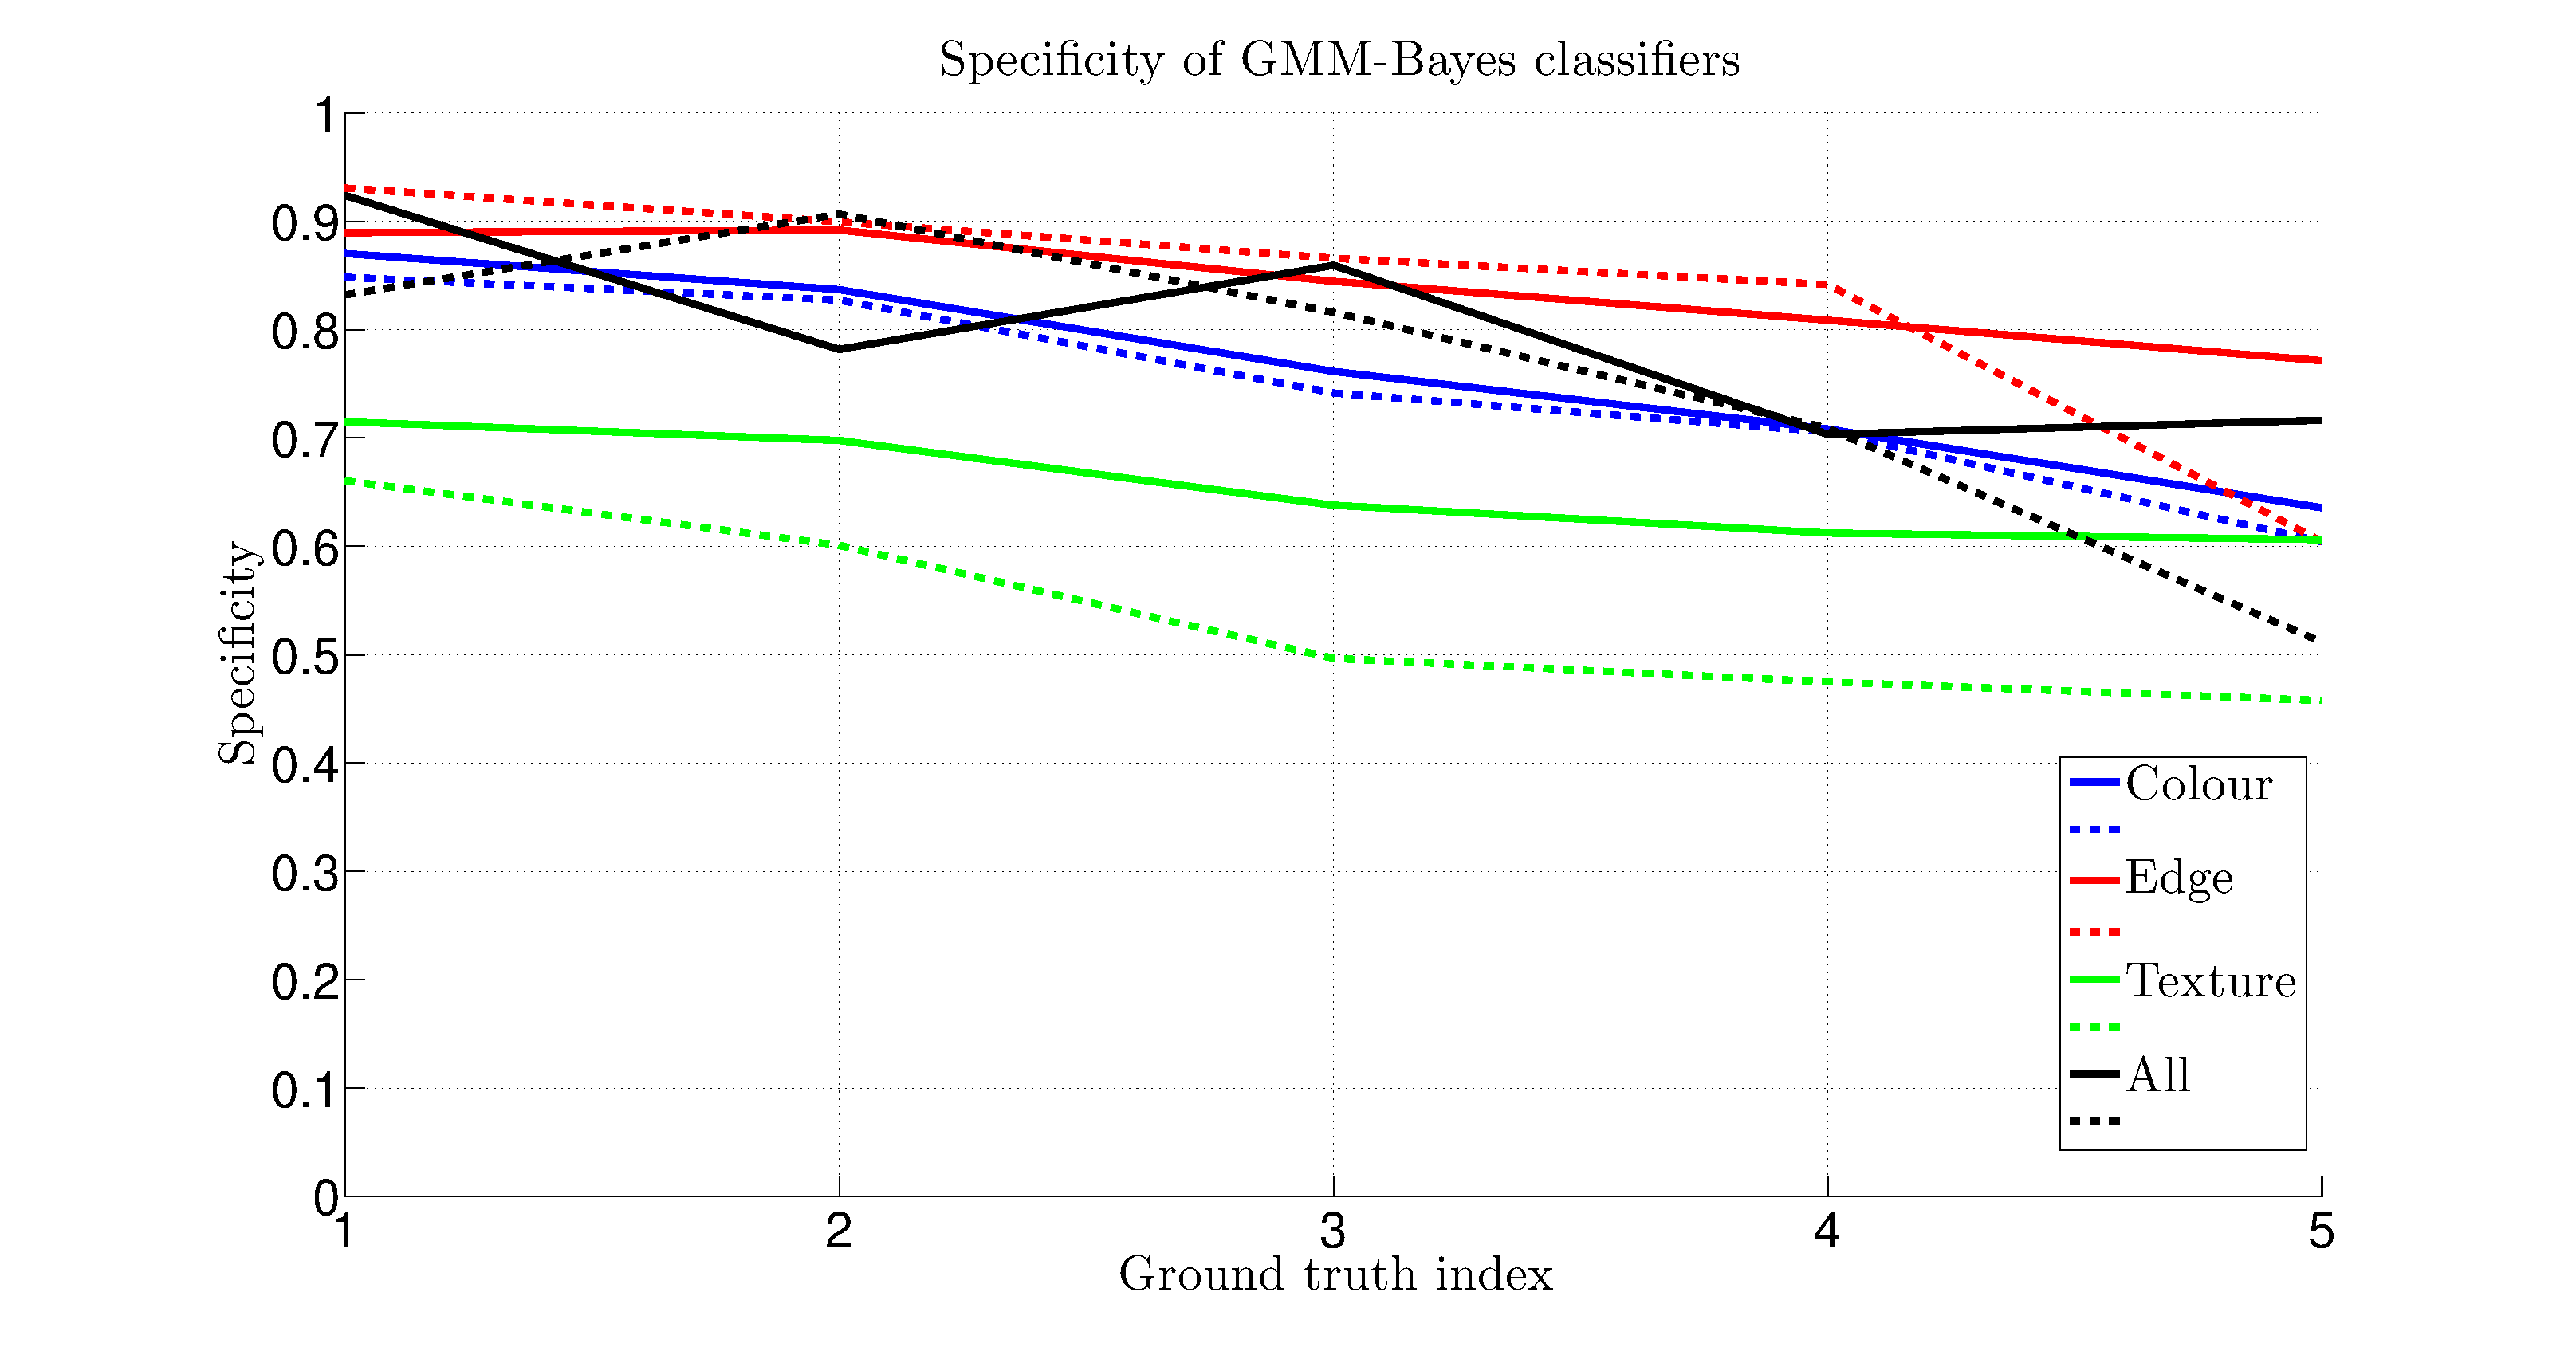
\includegraphics[width=0.95\textwidth]{hist_gmmbayes_spec_imgset2}
	}

	\caption[moving]{Performance of GMM-Bayes classifiers using gray world images:     
	\subref{fig:grayworld_gmmbayes_sens} sensitivity,
	\subref{fig:grayworld_gmmbayes_spec} specificity. }
	\label{fig:grayworld_gmmbayes}
    \end{figure}
\end{minipage}

\sectionend

\end{document}